\documentclass[12pt,openany,oneside,table]{cmuthesis}
\usepackage{float}
\usepackage{times}
\usepackage{fullpage}
\usepackage{graphicx, subfigure}
\usepackage{amsmath}
\usepackage{pifont}
\usepackage{amssymb}
\usepackage{multirow}
\usepackage{color}
\usepackage{verbatim}
\usepackage[numbers,sort]{natbib}
\usepackage[backref,pageanchor=true,plainpages=false, pdfpagelabels, bookmarks,bookmarksnumbered,
]{hyperref}
\usepackage{subfigure}
\usepackage{tikz}
\usepackage{xifthen}
\usepackage{adjustbox}
\usepackage{booktabs}
\usepackage{algpseudocode}
\usepackage{listings}
\usepackage{multirow}
\usepackage{enumitem}
\usepackage{xspace}
\usepackage{anyfontsize}


\usepackage{tabularx}
    \newcolumntype{L}{>{\raggedright\arraybackslash}X}
    \newcolumntype{s}{>{\raggedright\arraybackslash}m{2.8cm}}
\def\BibTeX{{\rm B\kern-.05em{\sc i\kern-.025em b}\kern-.08em
    T\kern-.1667em\lower.7ex\hbox{E}\kern-.125emX}}



\usepackage{fancybox}
\usepackage{csquotes}

\newcommand{\summary}[1]{
  \setlength{\fboxsep}{0.8em}
  \vspace{0.5em}
  \begin{center}
  \Ovalbox{\begin{minipage}{0.9\linewidth}
    \textbf{\emph{Summary.}} \emph{#1}
    \end{minipage}}
  \end{center}
  \vspace{0.5em}}
  
\newcommand{\vect}[1]{\boldsymbol{#1}}
\newcommand{\realnumbers}{\mathbb{R}}
\DeclareMathOperator*{\argmax}{arg\,max}
\DeclareMathOperator*{\argmin}{arg\,min}

\newcommand\No{\ding{56}}
\newcommand\Yes{\ding{52}}
\newcommand*\rot{\rotatebox{90}}
\usepackage[acronym]{glossaries}

\lstdefinelanguage{JavaScript}{
  keywords={typeof, new, true, false, catch, function, return, null, catch, switch, var, if, in, while, do, else, case, break, const, await, async, yield},
  keywordstyle=\color{blue},
  ndkeywords={class, export, boolean, throw, implements, import, this},
  ndkeywordstyle=\color{darkgray},
  identifierstyle=\color{black},
  sensitive=false,
  comment=[l]{//},
  morecomment=[s]{/*}{*/},
  commentstyle=\color{olive},
  stringstyle=\color{purple},
  morestring=[b]',
  morestring=[b]"
}
\lstdefinestyle{customjs}{
  language=JavaScript,
  extendedchars=true,
  basicstyle=\small\ttfamily,
  showstringspaces=false,
  showspaces=false,
  numbers=left,
  numberstyle=\footnotesize,
  % numbersep=-4pt,
  tabsize=2,
  breaklines=false,
  showtabs=false,
  captionpos=b,
  frame=single,
  framerule=0.2pt,
  morecomment=[l][\annotationcolor\bfseries]{\#},
  framexleftmargin=2em,
  xleftmargin=2.5em,
  xrightmargin=0.5em,
}

%%%%%%%%%%%%%%%%%%%%%%%%%%%%%%%%%%%%%%%%%%
% General
%%%%%%%%%%%%%%%%%%%%%%%%%%%%%%%%%%%%%%%%%%%

%% Comments
% \newcommand{\notes}[1]{}
% \newcommand{\TODO}[1]{}
\newif\ifshownotes
\shownotestrue
%\shownotesfalse

\ifshownotes
\newcommand{\notes}[1]{{\small \textsf{\textcolor{red}{[#1]}}}}
\newcommand{\TODO}[1]{\textcolor{red}{[TODO: #1]}}
\newcommand{\todo}[1]{\TODO{#1}}
\newcommand{\darion}[1]{\notes{Darion says: #1}}
\newcommand{\limin}[1]{\notes{Limin says: #1}}
\newcommand{\nuno}[1]{\notes{Nuno says: #1}}
\newcommand{\ruben}[1]{\notes{Ruben says: #1}}
\newcommand{\aidan}[1]{\notes{Aidan says: #1}}
\newcommand{\kevin}[1]{\notes{Kevin says: #1}}
\newcommand{\ronghao}[1]{\notes{Ronghao says: #1}}
\newcommand{\mindy}[1]{\notes{Mindy says: #1}}
\else
\newcommand{\notes}[1]{}
\newcommand{\TODO}[1]{}
\newcommand{\todo}[1]{}
\newcommand{\darion}[1]{}
\newcommand{\limin}[1]{}
\newcommand{\nuno}[1]{}
\newcommand{\ruben}[1]{}
\newcommand{\aidan}[1]{}
\newcommand{\kevin}[1]{}
\newcommand{\ronghao}[1]{}
\newcommand{\mindy}[1]{}
\fi



%% Formatting
\newcommand{\lilskip}{\vspace{.25\baselineskip}}

%% Boxes
\newcommand{\researchq}[2]{
\lilskip
\noindent\textbf{RQ#1}: #2
\lilskip
}
\newcommand{\researchqinline}[2]{\textbf{RQ#1}: #2}
\newcommand{\rqnum}[1]{\textbf{RQ#1}}

\newcommand{\resultbox}[2]{
\vspace{1mm}  \noindent\fbox{
    \begin{minipage}{0.96\columnwidth}
      \textbf{Result #1}: #2
    \end{minipage}%
  }%
  \vspace{1mm}
  }%

\newcommand{\textbox}[1]{
\vspace{1mm}  \noindent\fbox{
    \begin{minipage}{0.96\columnwidth}
      #1
    \end{minipage}%
  }%
}%

\newcommand{\headerbox}[2]{
\vspace{1mm}  \noindent\fbox{
    \begin{minipage}{0.96\columnwidth}
      \textbf{#1}: #2
    \end{minipage}%
  }%
}%

\newcommand{\codebox}[1]{\vspace{0.15cm} \\ #1 \vspace{0.15cm} \\}


%% References
\newcommand{\secref}[1]{Section~\ref{#1}}
\newcommand{\figref}[1]{Figure~\ref{#1}}
\newcommand{\tabref}[1]{Table~\ref{#1}}
\newcommand{\appref}[1]{Appendix~\ref{#1}}
\newcommand{\defref}[1]{Definition~\ref{#1}}
\newcommand{\algoref}[1]{Algorithm~\ref{#1}}
\newcommand{\chapref}[1]{Chapter~\ref{#1}}

%% Math
\newcommand{\m}[1]{\mathtt{#1}}

%% Theorem environments
% \newtheorem{theorem}{Theorem}
% \theoremstyle{plain}
% \newtheorem{thm}{Theorem}
% \newtheorem{lem}[thm]{Lemma}
% \newtheorem{cor}[thm]{Corollary}
% \newtheorem{defn}[thm]{Definition}
% \newtheorem{assumption}[thm]{Assume}
% \theoremstyle{definition}
% \newtheorem{definition}{Definition}[section]
% \newenvironment{proofsketch}{\noindent{\it Proof (sketch):}\hspace*{0.25em}}{ \hspace*{\fill} \qed}

%% Symbols
\makeatletter
\newsavebox{\@brx}
\newcommand{\llangle}[1][]{\savebox{\@brx}{\(\m@th{#1\langle}\)}%
  \mathopen{\copy\@brx\kern-0.5\wd\@brx\usebox{\@brx}}}
\newcommand{\rrangle}[1][]{\savebox{\@brx}{\(\m@th{#1\rangle}\)}%
  \mathclose{\copy\@brx\kern-0.5\wd\@brx\usebox{\@brx}}}
\makeatother


%%%%%%%%%%%%%%%%%%%%%%%%%%%%%%%%%%%%%%%%%%%
% NodeMedic
%%%%%%%%%%%%%%%%%%%%%%%%%%%%%%%%%%%%%%%%%%%

%% Acronyms
\newacronym{aci}{ACI}{Arbitrary Command Injection}
\newacronym{ace}{ACE}{Arbitrary Code Execution}
\newacronym{llms}{LLMs}{Large Language Models}

%% Project names
\newcommand{\nodemedic}{\textsc{NodeMedic}\xspace}
\newcommand{\nodemedicfine}{\textsc{NodeMedic-FINE}\xspace}
\newcommand{\name}{\textsc{NodeMedic-LM}\xspace}
\newcommand{\nameshort}{\textsc{NodeMedic-LM}\xspace}

%% Component names
\newcommand{\Enum}{Enumerator\xspace}

%% Node.js names
\newcommand{\nodejs}{{Node.js}\xspace}
\newcommand{\npmpkg}[1]{\emph{#1}\xspace}
\newcommand{\npm}{{npm}\xspace}

% Responsible disclosure of package names
% Comment for anonymization
% \newcommand{\cleartext}[1]{\npmpkg{#1}}
% \newcommand{\anontext}[1]{}
% Comment for de-anonymization
\newcommand{\cleartext}[1]{}
\newcommand{\anontext}[1]{\npmpkg{#1}}
\newcommand{\pkgname}[2]{\cleartext{#1}\anontext{#2}}

%% Symbols
\newcommand{\circled}[1]{\tikz[baseline=(char.base)]{\node[shape=circle,draw,inner sep=1.2pt] (char) {\scriptsize{#1}};}}

%% Code
%\lstinline[style=customjs]|exec|
\newcommand{\sink}[1]{\js{#1}}

%% Evaluation table circles
\newcommand*\emptycirc[1][1ex]{\tikz\draw[thick] (0,0) circle (#1);}
\newcommand*\halfcirc[1][1ex]{%
  \begin{tikzpicture}
  \draw[fill] (0,0)-- (90:#1) arc (90:270:#1) -- cycle ;
  \draw[thick] (0,0) circle (#1);
  \end{tikzpicture}}
\DeclareRobustCommand*\fullcirc[1][1ex]{\tikz\fill (0,0) circle (#1);}

%% space
\renewcommand{\paragraph}[1]{\vspace{0pt}\noindent{\bf #1}}

\usepackage{listings}
\usepackage{xcolor}
% \usepackage{inconsolata} % For a better monospaced font
\usepackage{tikz}
\usetikzlibrary{arrows.meta, shapes.geometric, positioning}

% Define JavaScript language for listings
\lstdefinelanguage{JavaScript}{
    keywords={function, var, require, if, else, return, try, catch},
    keywordstyle=\color{blue}\bfseries,
    ndkeywords={__set_taint__, exec},
    ndkeywordstyle=\color{orange}\bfseries,
    identifierstyle=\color{black},
    sensitive=false,
    comment=[l]{//},
    morecomment=[s]{/*}{*/},
    commentstyle=\color{gray}\itshape,
    stringstyle=\color{red},
    morestring=[b]',
    morestring=[b]"
}

% Settings for listings
\lstset{
    language=JavaScript,
    basicstyle=\ttfamily\footnotesize, % Use a better monospaced font
    breaklines=true,
    keywordstyle=\color{blue}\bfseries,
    stringstyle=\color{red},
    commentstyle=\color{gray}\itshape,
    numbers=left,                     % Line numbers on the left
    numberstyle=\tiny\color{gray},   % Line numbers styling
    frame=single,                    % Frame around the code
    captionpos=b,                    % Caption below the code
    xleftmargin=15pt,                % Margin on the left
    xrightmargin=15pt                % Margin on the right
}

\usepackage{pifont}
\newcommand{\cmark}{\checkmark} % Checkmark symbol
\newcommand{\xmark}{\ding{55}} % Cross symbol



\renewenvironment{quote}
%  {\small\list{}{\rightmargin=0.9cm \leftmargin=0.8cm}%
{\list{}{\rightmargin=0.5cm \leftmargin=0.5cm}
   \item\relax}
  {\endlist}
%\newcommand{\q}[1]{{\emph{``#1''}}}
\newcommand{\q}[1]{{\begin{quote}\emph{#1}\end{quote}}}
\newcommand{\ourq}[2]{\enquote{\emph{#2}} -- P#1}
\newcommand{\pquote}[2]{P#1 said: \q{#2}}

% Approximately 1" margins, more space on binding side
%\usepackage[letterpaper,twoside,vscale=.8,hscale=.75,nomarginpar]{geometry}
%for general printing (not binding)
\usepackage[letterpaper,twoside,vscale=.8,hscale=.75,nomarginpar,hmarginratio=1:1]{geometry}

\newcommand\afs[1]{\textcolor{orange}{AA: #1}}
\newcommand\clg[1]{\textcolor{blue}{CLG: #1}}
\newcommand\ct[1]{\textcolor{purple}{CT: #1}}
\newcommand{\signpost}[1]{{\color{gray}#1}}

\newcommand{\bpy}{\textit{BugsInPy}\xspace}
\newcommand{\devign}{\textit{Devign}\xspace}
\newcommand{\lstinlinegen}{\textit{CodeGen}\xspace}
\usepackage{tcolorbox}
\newcommand{\best}[1]{\hspace{-0.2cm}\colorbox{dawnblue}{\bf #1}}

\definecolor{deepblue}{rgb}{0,.2,0.6}
\definecolor{deepgreen}{rgb}{0,0.5,0}
\definecolor{deepchampagne}{rgb}{0.98, 0.84, 0.65}
\definecolor{mintgreen}{rgb}{0.6, 1.0, 0.6}
\definecolor{vividviolet}{rgb}{0.62, 0.0, 1.0}
\definecolor{mangotango}{rgb}{1.0, 0.51, 0.26}
\definecolor{dkgreen}{rgb}{0,0.5,0}
\definecolor{dkred}{rgb}{0.5,0,0}
\definecolor{gray}{rgb}{0.5,0.5,0.5}


\lstdefinestyle{javastyle} {
  language=Java,
  basicstyle=\ttfamily\bfseries\footnotesize,
  columns=flexible,
  morekeywords={virtualinvoke},
  keywordstyle=\color{blue},
  ndkeywordstyle=\color{red},
  commentstyle=\color{dkred},
  stringstyle=\color{dkgreen},
  numbers=left,
  breaklines=true,
  numberstyle=\ttfamily\footnotesize\color{gray},
  stepnumber=1,
  numbersep=10pt,
  backgroundcolor=\color{white},
  tabsize=4,
  showspaces=false,
  showstringspaces=false,
  xleftmargin=.23in,
  escapeinside={(*@}{@*)},
}

\lstset{style=javastyle}
% \colorlet{shadecolor}{gray!40}
% \sethlcolor{shadecolor}
% for starting line numbers
\newcommand*\startnumber[1]{%
    \setcounter{lstnumber}{\numexpr#1-1\relax}%
}
% for stopping line numbers
\newcommand*\stopnumber{%
    \startnumber{-2}%
}

% Provides a draft mark at the top of the document.
%\draftstamp{\today}{DRAFT}

\begin {document}
\frontmatter

%initialize page style, so contents come out right (see bot) -mjz
\pagestyle{empty}
\let\cleardoublepage\clearpage % Replace cleardoublepage with clearpage to avoid blank pages

\title{ {\it \huge Integrating Program Analysis with Language Models for Software Evolution}}
\author{Aidan Z.H. Yang}
\date{August, 2025}
\Year{2025}

\committee{
Claire Le Goues, Chair\\
Ruben Martins, Chair\\
Vincent Hellendoorn\\
Daniel Kroening
}


% copyright notice generated automatically from Year and author.We
% permission added if \permission{} given.

\keywords{automated program repair, program verification, large language models}

\maketitle

\pagestyle{plain} % for toc, was empty
\section*{Abstract}

Language models have improved by orders of magnitude with the recent emergence
of Transformer-based Large Language Models (LLMs). 
LLMs have demonstrated their ability to generate ``natural'' code that is highly similar to code written by
professional developers. 
However, the software engineering process involves much more than writing code: modern software evolves and requires continuous maintenance, such as debugging, or transpilation. 
For a LLM to assist in the software engineering process, it is important to build tools around a LLM to enable its ability to provide support for software evolution.
In this thesis proposal, we propose mechanisms to improve the utility of LLMs for software evolution by using and combining LLMs with prior APR and program verification techniques. Specifically, we build LLM-based software engineering tools for fault localization, program repair, and program transpilation.


My thesis statement is:
software engineering is an evolving process, including testing, debugging, and migration. Open-source, code assisting language models are commonly pre-trained on causal code generation (i.e., left-to-right). This limits their value in software maintenance and evolution tasks, which require a wholistic understanding of software properties. Adding an understanding of software properties through program analysis can assist in important steps of the software evolution process and mitigate the limitations of a language model.

To support this statement, we make the following contributions. 

I first propose and evaluate a bidirectional fine-tuning technique that enables a previously left-to-right LLM to locate and rank faulty lines of code. We built the LLM-based fault localization technique without depending on preciously written tests, and so the tool can also detect run-time security vulnerabilities. 

I further study a LLM's ability for program repair by combining the LLM's intermediate entropy values with traditional program repair techniques. In particular, we used LLM entropy values to improve three stages of program repair: fault localization, patch testing efficiency, and plausible patch ranking. Finally, we created a tool for fully automated Rust function transpilation using LLMs and verification harnesses. To support our claims, we evaluated all our LLM-based software evolution tools on real world bugs, security vulnerabilities, and target transpilation repositories.

I extend our study of LLM-based fault localization by adding mechanisms for multi-task LLM instruction-tuning, and evaluating the model on real-world security vulnerabilities in large repositories. Specifically, the completed fault localizer only detects faults on a line level, and does not take into account various nuances of security vulnerability explanations. LLMs have the capability of training on multiple objectives, including both recognizing the vulnerable lines of code, and the explanation of exploits occurring from a type of vulnerability. The completed vulnerability detector attempts to detect vulnerabilities that span across different files across aa larger repository. 

\begin{acknowledgments}
    I would like to thank my PhD advisors Claire Le Goues, Ruben Martins, and Vincent Hellendoorn for their mentoring, guidance, and patience. My parents Yin Chen and Yong Yang for encouraging me to start this PhD journey from an early age. My collaborators and mentors:
    Ansong Ni, Brandon Paulsen, Daniel Kroening, Daniel Ramos, Darion Cassel, He Ye, Haoye Tian, Joey Dodds, Limin Jia, Ronghao Ni, Soongho Kong, Sophia Kolak, Yoshi Takashima, and Zhizhen Qin. My partner Samantha Hong, and everyone at S3D and SquaresLab for supporting me through my PhD.
\end{acknowledgments}

\tableofcontents
%\listoffigures
%\listoftables

\let\cleardoublepage\clearpage % Replace cleardoublepage with clearpage to avoid blank pages
\mainmatter

%% Double space document for easy review:
%\renewcommand{\baselinestretch}{1.66}\normalsize

\chapter{Introduction}
\label{ch:intro}

Software is constantly evolving, requiring constant care from software engineers to maintain software quality. The software evolution process includes bug finding, bug fixing, and sometimes an entire overhaul of the software project (e.g., a change in the programming language used).
The problem of software evolution has motivated the development of a variety of
techniques for Automatic Program Repair (APR)~\cite{TBar, long_ml_patch,
patch_learning, claire_apr,patch-sim}. At a high level, dynamic APR approaches
use test cases to define a defect to be repaired and functionality to retain,
and to localize the defect to a smaller set of program lines.
Specifically, fault localization (FL)~\cite{abreu2007accuracy,li2019deepfl,lou2021boosting,li2022fault} approaches aim to automatically identify which program entities (like a line, statement, module, or file) are implicated in a particular bug. The goal is to assist programmers in fixing defects by pinpointing the places in the code base that should be modified to fix them. 
Broadly speaking, existing FL techniques combine or leverage
static and dynamic program analysis information to compute a score corresponding to a program entity's probability of contributing to a particular bug. 

Meanwhile, the recent advances in deep learning (DL) and AI have produced significant performance improvements over
previous machine learning techniques for code generation~\cite{Codex,Neox}. DL therefore
affords promising opportunities for program repair~\cite{long_ml_patch,
patch_learning, Infill_repair,Interfix,Prompt_repair} and fault localization~\cite{Llmao}.
The most effective DL models for both natural language and code related tasks are large language models (LLMs), such as Codex~\cite{chen2021evaluating} and GPT-4~\cite{openai2023gpt4}.
This class of models trains many billions of parameters with even more tokens of training data, which tends to yield highly flexible and powerful text generators.
LLMs' utility for code generation and the fact that they are trained on an abundance of publicly-available code~\cite{chen2021evaluating} both suggest that existing large-scale LLMs capture program source code in ways that can be leveraged for specialized development tasks.
A key property of LLMs is that their performance improves consistently with the \emph{scale} of their computational budget \cite{kaplan2020scaling}, which is itself a function of the model and training data size.
However, LLMs are not immediately suited off-the-shelf for coding tasks that do not involve code generation, like fault localization. 

% State-of-the-art LLMs for code~\cite{chen2021evaluating, black2021gpt, tunstall2022natural, nijkamp2022codegen} are trained to generate code in a left-to-right manner, with each token predicted from its preceding context. 
% I posit that models trained in this way are less suitable for token-level discriminative tasks, like line-level fault localization, because the representation for any given token is only conditioned on the context to the left. 

To expand to the problem of automated program repair (APR), we believe that solely fine-tuning a LLM is not enough. The fundamental idea behind using an LM alone - even a hypothetically optimal one - for repair treats predictability as ultimately equivalent to correctness.
This assumption is specious: LLMs adopt preferences based on a corpus
with respect to training loss that rewards imitation. Beyond the fact that LLMs
necessarily train on buggy code, LLMs generate and score text one token at the
time. Given that, they may well prefer a subtly incorrect implementation spread
across several readable lines over a correct but difficult-to-understand one-line
solution, as the per-token probability of the former may be strictly lower than the
latter. Judgment of code correctness requires substantially more context than an
LLM has access to including, but not limited to, test cases test behavior, and
developer intent. Although some of this information could be provided as context,
it will lie outside the training distribution. We argue that a careful combination of more traditional APR techniques with LLMs can produce the most effective results at all stages of APR.

As previously discussed, LLM-based approaches tend to produce code that is similar to their training data, and thus, if the model is trained on high quality, human written, code, the model will usually produce high quality, idiomatic code~\cite{yang2024revisiting}. This gives the insight that LLMs can be powerful code transpilation tools (i.e., migrating from one programming language to another that directly compiles). A LLM can take a program in one language as input and attempt to output an equivalent program in the target
language~\cite{roziere2020unsupervised}. However, directly prompting a LLM comes with no formal guarantees that the resulting code will maintain input-output equivalence with the original~\cite{consistency, xu2024hallucination, pan2024lost}. Due to the unique nature of code transpilation, in which program equivalence can be represented by equivalence input-output pairings, we show that a LLM can produce verified transpilation when surrounded by test-harnesses and undergoing both testing and verification.

My key insight through building tools for fault localization, program repair, and program transpilation is that a LLM acts as a black box model for code generation, which can only be trusted when combined with non-ML based software engineering techniques.

\section{Thesis Statement}

Software engineering is an evolving process, including testing, debugging, and migration. Open-source, code assisting language models are commonly pre-trained on causal code generation (i.e., left-to-right). This limits their value in software maintenance and evolution tasks, which require a wholistic understanding of software properties. Adding an understanding of software properties through program analysis can assist in important steps of the software evolution process and mitigate the limitations of a language model.

\section{Contributions}

This proposal contains a set of prototypes for addressing common software engineering tasks that are apart of a software's evolution.
My thesis will contribute in the following ways:
\begin{enumerate}
\item
It introduces a fault localization specific LLM, while trained using light-weight bidirectional adapter layers.
\item
It shows that the entropy values from various LLMs, when combined with prior APR tools, can improve upon all stages of APR as compared to either a LLM or traditional APR tool in separation.
\item
It provides a set of techniques to safe-guard against LLM hallucinations for code-generation, which I evaluate on the task of transpiling to the Rust programming language.
\end{enumerate}




\chapter{Background and Related Works}
\label{ch:background}

The following sections give an overview of related work and background
that inform the proposed work.

\section{LLM for code}
Language models have been used for code generation, bug detection, and patch
generation. Recent language models finetune on code as training data and can
perform code completion~\cite{desai2016program, inCoder}, and generate code
based on natural language~\cite{raychev2014code} with impressive results. Large
Language Models (LLMs), such as Codex~\cite{Codex}, GPT-Neo~\cite{Neox}, and
Llama-2~\cite{Llama} have raised performance on these tasks by using more
trainable parameters and training data. Ray et al.~\cite{NAT} study the
relationship between bugginess and LLM-entropy. Ray et al. empirically showed
that n-gram models trained over a large corpus of code will find buggy
statements more surprising, as indicated by a high entropy score. 
Kolak et
al.~\cite{LLM-PATCH} revisit the question of naturalness (i.e., the
human-readability) of patches in the era of large language models. Kolak et al. experimented with models ranging from [160M to 12B] parameters, and measured the similarly between LLM generated patches and developer written patches. Their
results show that larger models tend to generate test-passing lines at a higher
rate. Additionally, LLM generated patches tend to be more similar to the
human-written patch as model size increases. Xia et al.~\cite{xia2023automated} directly applied LLMs for APRs and found that LLMs can suggest multi-line fixes with higher accuracy than state of the art APR tools. Xia et al.~\cite{xia2023automated} concluded that while LLMs can often perform localization and generation in one shot, it is significantly more cost-effective to use traditional FL first/instead, motivating our work. 

\section{Fault Localization}
Prior fault localization tools use test output information, code semantics, and
naturalness of code to achieve a high degree of confidence on bug detection.
Spectrum-based Fault Localization (SBFL)~\cite{abreu2006evaluation,
abreu2007accuracy} uses a ratio of passed and failed tests covering each line of
code to calculate its suspiciousness score, in which a higher suspiciousness
signifies a higher probability of being faulty. Recent advances in deep learning
created a spur of research on using graph neural networks (GNNs)~\cite{GNN} for
fault localization. GRACE~\cite{Grace}, DeepFL~\cite{DeepFL}, and
DEAR~\cite{Dear} encode the code AST and test coverage as graph representations
before training deep learning models for fault localization.
TransferFL~\cite{TransferFL} combined semantic features of code and the
transferred knowledge from open-source code data to improve the accuracy of
prior deep learning fault localization tools.

\section{Patch correctness}
Similarly to prior fault localization tools, prior patch disambiguation tools
leverage test output information and code information (both code syntax and code
semantics) for ranking or classifying patches. Qi et al.~\cite{qi2015analysis} analyzed the reported
bugs of three generate-and-validate APR tools: GenProg~\cite{genprog},
RSRepair~\cite{rsrepair}, and AE~\cite{ae} systems, to find that producing
correct results on a validation test suite is not enough to ensure patch
correctness. Smith et al.~\cite{CURE} performed
an experiment that interrogates whether or not automatically generated patches
are prone to overfitting to their test suite. Borrowing the concept of training
and test sets from machine learning, they found that automated program repair
(APR) typically used the same test-suite for both ``training" (generating the
patch), and ``testing" (validation). Smith et al. found that both the coverage
rate of the test-suite, as well as the assignment of test/train sets between the
two suites, impact the degree of overfitting in repair. To counteract the
overfitting problem, Ye et al.~\cite{ye_patches} proposed ODS (Overfitting
Detection System), a novel system to statically classify overfitting patches.
Xiong et al.~\cite{patch-sim} generated both execution traces of patched
programs and new tests to assess the correctness of patches. Ghanbari et
al.~\cite{Shibboleth} used both the syntactic and semantic similarity between
original code and proposed patch, and code coverage of passing tests to rank
patches. Shibboleth~\cite{Shibboleth} was able to rank the correct patch in
Top-1 and Top-2 positions in 66\% of their curated dataset. Tian et
al.~\cite{Panther} proposed machine learning predictor with BERT
transformer-based learned embeddings for patch classification. Tian et al. found
that learned embeddings of code fragments with BERT~\cite{BERT},
CC2Vec~\cite{cc2vec}, and Doc2Vec~\cite{doc2vec} yield similarity scores that,
given a buggy code, substantially differ between correctly-patched code and
incorrectly-patched one. 
Yang et al.~\cite{yang2023large} found that state-of-the-art learning-based techniques suffered from the dataset overfitting problem, and that naturalness-based
techniques outperformed traditional static techniques, in particular
Patch-Sim~\cite{patch-sim}.


\section{Equivalence verification}
Equivalence verification has been studied in settings where two copies
of should-be-equivalent artifacts are available: compiler
optimizations~\cite{churchill_semantic_2019,churchill_sound_2017} and program
verification~\cite{antonopoulos_algebra_2023,kommrusch_self-supervised_2023}. Our
work uses equivalence verification for program language
translation.


\section{Rust transpilers}
Prior Rust transpilers convert C/C++ to Rust.  C2Rust~\cite{C2Rust}
automatically converts large-scale C programs to Rust while preserving
C semantics. Citrus~\cite{citrus} and Bindgen~\cite{bindgen} both
generate Rust FFI bindings from C libraries, and produce Rust code
without preserving C semantics. Bosamiya et
al.~\cite{bosamiya2022provably} embedded WebAssembly (Wasm) semantics
in safe Rust code for the Rust compiler to emit safe and executable
Rust code. Bosamiya et al.~\cite{bosamiya2022provably} implemented all
stages of their tool in safe Rust, and no stage of compiler needs to
be further verified or trusted to achieve safety.
Existing tools for making unsafe Rust safer focus on converting raw
pointers to safe references. Emre et al.~\cite{emre2021translating}
localized unsafe Rust code from C2Rust and converted unsafe Rust to
safe Rust by extracting type and borrow-checker results from the
\texttt{rustc} compiler. Zhang et al.~\cite{zhang2023ownership}
converts unsafe Rust from C2Rust to safe Rust by computing an
ownership scheme for a given Rust program, which decides which
pointers in a program are owning or non-owning at particular
locations. Zhang et al.~\cite{zhang2023ownership} evaluates their tool
CROWN on a benchmark suite of 20 programs, and achieve a median
reduction rates for raw pointer uses of 62.1\%.  Ling et
al.~\cite{ling2022rust} removed non-essential ``unsafe'' keywords in
Rust function signatures and refined the scopes within unsafe block
scopes to safe functions using code structure transformation. Our work
is the first to propose a general Rust transpiler that does not depend
on the source language's memory management properties to produce safe
Rust.
\section{Software vulnerability detection}
Security vulnerability detection has a rich research history covering both static and dynamic techniques (see., e.g., ref~\cite{sokMemory,secVulSurvey,fuzzingSurvey}). 
For example, code-similarity-based methods~\cite{vuddy, vulpecker} can detect vulnerabilities incurred by code cloning, and pattern-based methods~\cite{neuhaus2007predicting, chucky} use rules to identify vulnerabilities based on code patterns. However, code-similarity techniques show high false negative rates (many vulnerabilities are not caused by cloning), 
and pattern-based techniques require human experts to define the initial patterns. 
We focus on work using machine learning for static vulnerability detection, as it is most closely related to ours, requires less human expert intervention, and recent results are especially promising.

Devign~\cite{zhou2019devign} and IVDetect~\cite{ivdetect} used GNN on a program's AST or CFG to learn a program's likelihood to be vulnerable. LineVul~\cite{linevd} queried the final attention layers of a language model (CodeBERT) for the specific purpose of vulnerability detection. 
DeepDFA~\cite{deepdfa} uses DFA algorithms to train a GNN and achieve state-of-the-art vulnerability detection results more efficiently than prior program analysis based tools. Steenhoek et al.~\cite{deepdfa} observed that DeepDFA, when combined with LineVul~\cite{linevd}, yields a higher vulnerability detection effectiveness than all prior Transformer-based tools.



\subsection{\nodejs Package Threat Model}
\label{sec:background:threat-model}
\nodejs is %a JavaScript runtime 
built on top of the V8 JavaScript engine. \nodejs developers combine code into {\em packages}, which
can import other packages as \emph{dependencies} to use their public APIs (exported functions).
%
\nodejs provides powerful \emph{sensitive APIs}~\cite{eval_fn,new_function_fn,exec_fn,execsync_fn} that 
%allow programmers to perform 
can dynamically generate code and execute shell commands.

\begin{figure}[t!]
  \centering
  \vspace{-3pt}
  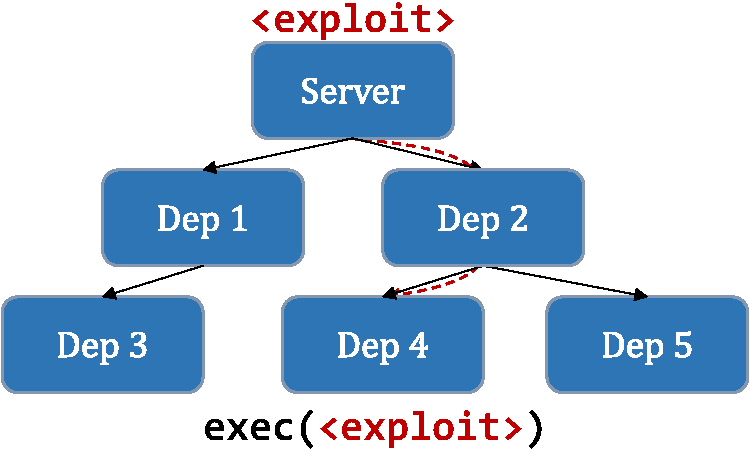
\includegraphics[width=0.5\columnwidth]{figures/approach/attacker_model.pdf}
  \vspace{-5pt}
  \caption{Arrows represent a \emph{depends on} relationship.
    A victim application (Server) passes 
    attacker-controllable input ($\m{exploit}$) to its vulnerable dependency, 
    Dep 4 (dataflow indicated by dashed red arrows).}
  \vspace{-5pt}
  \label{fig:attacker-model}
\end{figure}

In a real-world attack, 
a \nodejs package that unsafely uses sensitive 
\nodejs APIs is included as a \emph{dependency} of a \emph{victim} application as illustrated in \figref{fig:attacker-model}.
An attacker can be any user communicating with the 
victim application.
Attacker-controlled input is passed
from the victim application to the dependency's public API, which passes it to a
sensitive API (e.g., \lstinline|exec|~\cite{exec_fn}).
We utilize an idealized model of the above scenario that echoes trust assumptions in prior work~\cite{staicu-SYNODE,nodemedic-fine,cassel2023nodemedic}. 
The attacker \emph{directly} passes input to the dependency.
We consider \emph{all} public APIs of the dependency to be the attack surface of the package.
We scope this work to focus on two types of severe attacks: arbitrary code execution (\gls{ace})~\cite{cwe_94}
and arbitrary command injection (\gls{aci})~\cite{cwe_77}. An attacker capable of these can launch
other attacks, e.g., directory traversal~\cite{cwe_22}, by extension.

\subsection{Dynamic Taint Analysis}
Taint analysis specifies and checks policies governing \emph{sensitive 
dataflow} with programs. A goal of the analysis is to detect flows from particular \emph{sources}, e.g., 
API inputs, to \emph{sinks}, e.g., functions with dangerous capabilities such as command execution.
Taint analysis that runs during program execution is termed dynamic
taint analysis. 
Dynamic taint analysis has been particularly efficacious for detecting code vulnerabilities of 
JavaScript (c.f.~\cite{andreasen-Survey}).

Several tools perform taint analysis of \nodejs
packages~\cite{karim-PlatformIndependent,nielsen-Nodest,gauthier-AFFOGATO,song_ObjLupAnsys,ming_taintpipe,jsprime_2013,staicu-Extracting}.
We focus on leveraging \nodemedicfine~\cite{nodemedic-fine}, which implements a taint
\emph{provenance analysis}, wherein a history of operations applied to tainted
data is saved as \emph{provenance graph} (more details in Section~\ref{subsec:provenance-analysis}) and can be used for further analysis. 
\nodemedicfine uses the provenance graph for synthesizing proof of concept exploit to confirm the vulnerability. 
This work uses the provenance graph as input to a set of ML methods for vulnerability detection.



\subsection{Provenance Graph}
\label{subsec:provenance-analysis}

Provenance graphs generated by \nodemedicfine are data structures constructed through dynamic taint analysis that capture the complete history of operations applied to tainted values during a program’s execution. 
Each node in a provenance graph represents a taint-related operation or value, while edges illustrate the flow of data between these nodes.

We reuse the toy package \texttt{toygrep} from \nodemedic{} \cite{cassel2023nodemedic} as an illustrative example to demonstrate how \nodemedic generates the provenance graphs using package source code and driver programs. This toy example (shown in Listing \ref{lst:toy_code}) exposes an API function called \texttt{grep}, which takes an argument \texttt{query} and executes the system command \texttt{grep [query]} without any sanitization.

The driver program (shown in Listing \ref{lst:driver_program}) simulates the behavior of an external input by creating a variable \texttt{x} marked as tainted using the \texttt{\_\_set\_taint\_\_} function. Then this tainted variable is passed as the \texttt{query} argument to the \texttt{grep} function, triggering the execution of the system command.

\begin{figure}[h]
    \centering
    \vspace{-0.5em}
    % Left side: Two code listings stacked vertically (wider column)
    \begin{minipage}{0.64\linewidth}  % Increase width for code
        \centering
        \begin{lstlisting}[language=JavaScript, caption=Source code for the toy package \texttt{toygrep}, label=lst:toy_code]
function grep(query) {
    exec("grep " + query);
}
        \end{lstlisting}

        \vspace{0.5cm} % Add spacing between the two listings

        \begin{lstlisting}[language=JavaScript, caption=Driver program for the toy package \texttt{toygrep}, label=lst:driver_program]
var PUT = require("toygrep");
var x = "tainted"; // {0:'0'}
__set_taint__(x);
try{PUT.grep(x);}
catch (e) {console.log(e)}
        \end{lstlisting}
    \end{minipage}
    \hfill
    % Right side: Corrected Vertical Provenance Graph with Curved Arrow
    \begin{minipage}{0.34\linewidth}  % Reduce width for graph
        \centering
        \begin{tikzpicture}[
            scale=0.93, % Reduce overall scale
            node distance=1.2cm, % Adjust vertical spacing
            every node/.style={draw, align=center, font=\small, ellipse, minimum height=0.8cm, minimum width=2.5cm, transform shape},
            normal/.style={draw=black},
            taintededge/.style={-{Stealth}, thick, red},
            untaintededge/.style={-{Stealth}, thick, black},
            taintflow/.style={-{Stealth}, thick, red}
        ]

        % Nodes (Maintaining correct flow)
        \node[normal] (n1) {Untainted \\ {[String: 'grep ']}};
        \node[normal, below=0.7cm of n1] (n2) {call:grep \\ 'tainted'};
        \node[normal, below=0.6cm of n2] (n3) {string.concat \\ 'grep tainted'};
        \node[normal, below=0.6cm of n3] (n4) {call:exec \\ 'grep tainted'};

        % Correct edges (Maintaining the taint propagation paths)
        \draw[taintededge] (n2) -- (n3);  % Tainted input to concatenation
        \draw[taintflow] (n3) -- (n4);  % Tainted execution propagation

        % Self-loop for call:grep to show taint persistence
        \draw[taintflow] ([xshift=-1.2cm, yshift=0.4cm]n2.north) to[out=0, in=90] (n2.north);

        % Special curved edge to bypass n2 (from n1 to n3, passing across n2)
        \draw[untaintededge] (n1.south east) to[out=-50, in=50] (n3.north east);

        \end{tikzpicture}
        \label{fig:corrected-toy-provenance-graph}
    \end{minipage}
    \caption{Provenance graph generated from the \texttt{toygrep} package.
    % and its source code and driver program. 
    Upper-left section contains source code (Listing \ref{lst:toy_code}); Bottom-left section contains the driver program (Listing \ref{lst:driver_program}); Right section presents the provenance graph. A circle is a node. Black edges are untainted, red edges are tainted flows.}
    \label{fig:toy-provenance-graph}
    \vspace{-0.5em}
\end{figure}
Figure \ref{fig:toy-provenance-graph} shows the provenance graph generated from the vulnerable toy package \texttt{grep} and its driver program. The graph illustrates how the input flows through the \texttt{grep} function call, is concatenated with the string \texttt{grep}, and ultimately reaches the sink, \texttt{exec}.
Each node in a provenance graph captures key details about the operations and data flow within the program. Table~\ref{tab:node_attributes} provides an overview of these attributes.

\begin{table}[h]
\centering
\caption{Attributes of nodes in provenance graphs.\label{tab:node_attributes}}
\begin{tabular}{@{}ll@{}}
\toprule
\textbf{Attribute}          & \textbf{Description}                       \\ \midrule
Operation         & Type of operation, e.g., \texttt{call} or \texttt{Untainted}. \\ \midrule
Value             & Input provided to the operation.           \\ \midrule
File Path         & File where the operation occurs.           \\ \midrule
Position          & Start and end line/column in the file.     \\ \midrule
Tainted Status    & Whether the data is tainted or untainted.  \\ \midrule
Flows From        & Predecessor nodes in the data flow.        \\ \midrule
Sink Type         & \texttt{spawn} or \texttt{exec}. \\ \bottomrule
\end{tabular}
\end{table}



\chapter{Fault localization}
\label{ch:llmao}

% This section describes parts of the completed work of this thesis proposal.

Debugging is an important step in the software maintenance process, and the first step in debugging is finding where the bug occurs in a software repository.
As described in Chapter~\ref{ch:intro}, fault localization (FL) approaches aim to automatically identify which program entities (like a line, statement, module, or file) are implicated in a particular bug. The goal is to assist programmers in fixing defects by pinpointing the places in the code base that should be modified to fix them. 
However, LLMs are not immediately suited off-the-shelf for coding tasks that do not involve code generation, like fault localization. State-of-the-art LLMs for code~\cite{chen2021evaluating, black2021gpt, tunstall2022natural, nijkamp2022codegen} are trained to generate code in a left-to-right manner, with each token predicted from its preceding context. 
Models trained in this way are less suitable for token-level discriminative tasks, like line-level fault localization, because the representation for any given token is only conditioned on the context to the left. 

We present a promising alternative: we train lightweight bidirectional \emph{adapters}, themselves small models of the same architecture as the base LLM, on top of left-to-right language models. These adapters add relatively few parameters and can be trained effectively on small datasets of real bugs, such as \textit{Defects4J}~\cite{just2014defects4j}, without updating the underlying LLM. We demonstrate that the representations learned by pretrained left-to-right language models already contain a wealth of knowledge about the suspiciousness of lines of code, which increases strongly with the size of the LLM.  I can leverage this power through our adapters to find bugs while requiring just a few hundred training samples for pretraining. 
our approach yields better fault localization performance than prior work while requiring significantly less data preprocessing overhead. Importantly, our approach does not use test cases at all, and therefore does not depend on test code quality for its performance. 

\section{LLMAO: Large Language Models for Fault Localization}
\label{sec:LLMAO}

\begin{figure*}
\centering
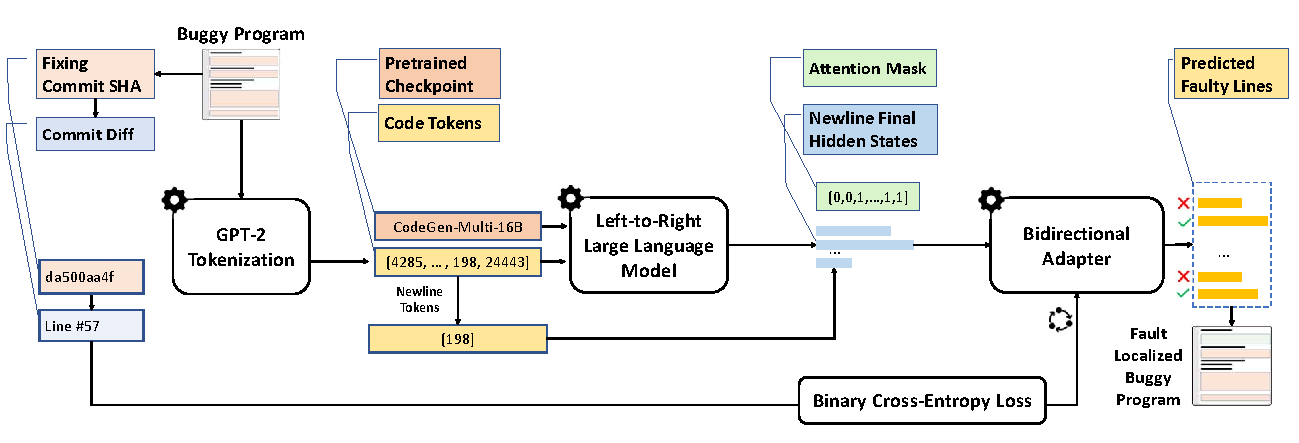
\includegraphics[width=\textwidth]{figures/approach/overview.pdf}
%\vspace*{-3mm}
\caption{\small \textit{LLMAO}’s architecture, which takes as input a buggy program and produces a list of suspiciousness scores for each code line}
\label{fig:overview-llmao}
\end{figure*}

In this section, we discuss the key ideas behind our language model enabled fault localization technique.
Figure \ref{fig:overview-llmao} shows an overview of \textit{LLMAO}'s training setup. The input to \textit{LLMAO} is a buggy program; its output is a list of \emph{suspiciousness} scores corresponding to each code line's probability of being buggy -- values close to 1 indicate that lines are likely defective. As shown in Figure \ref{fig:overview-llmao}, we first tokenize the input and then provide it to a pretrained left-to-right LLM. From this LLM, we obtain one (high-dimensional) \emph{vector representation} per line, which I provide to a small bidirectional model that predicts bugginess probabilities for each line. We only train the final stage of this model; the LLM remains frozen and can be easily replaced with other powerful open-source models. Figure \ref{fig:attention} shows a more detailed description of our language modeling procedure, which I describe in detail in Section \ref{sec:adapter}.
In the following sections, we describe each component of \textit{LLMAO}.
    
\subsection{Left-to-right Language Models}
Neural Language Models typically produce text in a left-to-right manner, producing each word given its prefix context. This both enables efficient training, as any document can be turned into a collection of as many training samples as there are tokens, and enables them to generate new text once trained.
Virtually all modern language models are attention-based models that use the Transformer architecture \cite{vaswani2017attention}. In these models, each token exchanges information with all other tokens via a learned attention procedure. To efficiently train left-to-right Transformer models on an entire document in which each token is generated only from its prefix context thus involves ``masking out'' part of the attention matrix to prevent each token from attending to its suffix context (essentially, the future). 
Figure \ref{fig:attention} (top) shows the causal attention mechanism used to train a left-to-right language model. 
Figure \ref{fig:attention} describes a simplified Transformer model for both \textit{CodeGen} and our bidirectional language model.
Auto-regressive and left-to-right LMs~\cite{chen2021evaluating, black2021gpt, tunstall2022natural, nijkamp2022codegen} use all previous tokens (i.e., tokens to the left) to predict the probability of the next token (i.e., tokens to the right).
Left-to-right models are useful for program generation tasks, as shown in Figure \ref{fig:attention}.
Specifically, the lower triangular part of the attention matrix remains unmasked (visualized as blue) while attention in the remaining part is masked out (white). This configuration allows each token to attend to itself and all past tokens, but prevents it from attending to future tokens.

our approach is compatible with any left-to-right language model, but is most effective when the underlying model is large and has been pretrained on a large volume of code data. At present, the \textit{CodeGen} family of models~\cite{nijkamp2022codegen} is most suitable for this role. These are a series of increasingly large left-to-right language models trained for program synthesis in three stages:
\begin{enumerate}
    \item{Each model is first trained on the natural language dataset ThePile, an 825.18 GiB mostly English language text corpus collected by Gao et al.~\cite{gao2020pile} for language modeling. 7.6\% of the dataset is programming language data collected from GitHub repositories with more than 100 stars.}
    \item{The models are then further trained on data from the Google BigQuery GHArchive dataset, which consists of open-source code across multiple programming languages -- C, C++, Go, Java, JavaScript, and Python.}
    \item{Finally, the models are tuned on the BIGPYTHON dataset, which contains a large amount of Python data.}
\end{enumerate}
Checkpoints after each stage are released for every model size, ranging from 350M to 16B parameters. The 16B model outperforms the original Codex model \cite{chen2021evaluating} on a Python program synthesis task.

While language models are typically used to predict the next token, they can also return the ``hidden'' states from their final Transformer layer. When generating text, these states are converted to a next-token prediction via a simple linear transformation. As such, these states tend to represent the model's knowledge about the evolving context at each point in the file, making them intrinsically useful. As shown in Figure \ref{fig:attention}, we extract the final hidden states for each newline (NL) token in each training sample from CodeGen to produce a condensed sequence representation in which each token represents one line. We pair these with their corresponding location (i.e., line \#5 of a 50 line file) and save these to disk.

To train our model, we load these encoded lines in batches, where I retrieve samples of up to 128 contiguous newline states at a time. We choose this number because the \textit{CodeGen} model can consume a maximum of 2,048 tokens as its input size; inputs with 128 lines almost always fit this token budget. Samples with fewer lines are padded, along with the label vector, to obtain a uniform length. Padding entries are ignored in the loss computation. When files contain more than 128 lines, we sample a series of 128 line windows that cover each faulty line in the file. Specifically, we repeatedly create a sample with up to 128 lines starting from a random offset before the immediate next faulty lines that is not yet covered by a previous segment. We then mark all faulty lines in this segment as covered and repeat until all lines are covered by at least one segment. We choose random starting offsets to ensure that the faulty lines within the split code lines are not consistently at the same indices (e.g., right at the start or in the middle), which would cause our model to memorize certain index locations as faulty lines.  This enables our technique to handle inputs longer than 2048 tokens.


\begin{figure}[t]
\centering
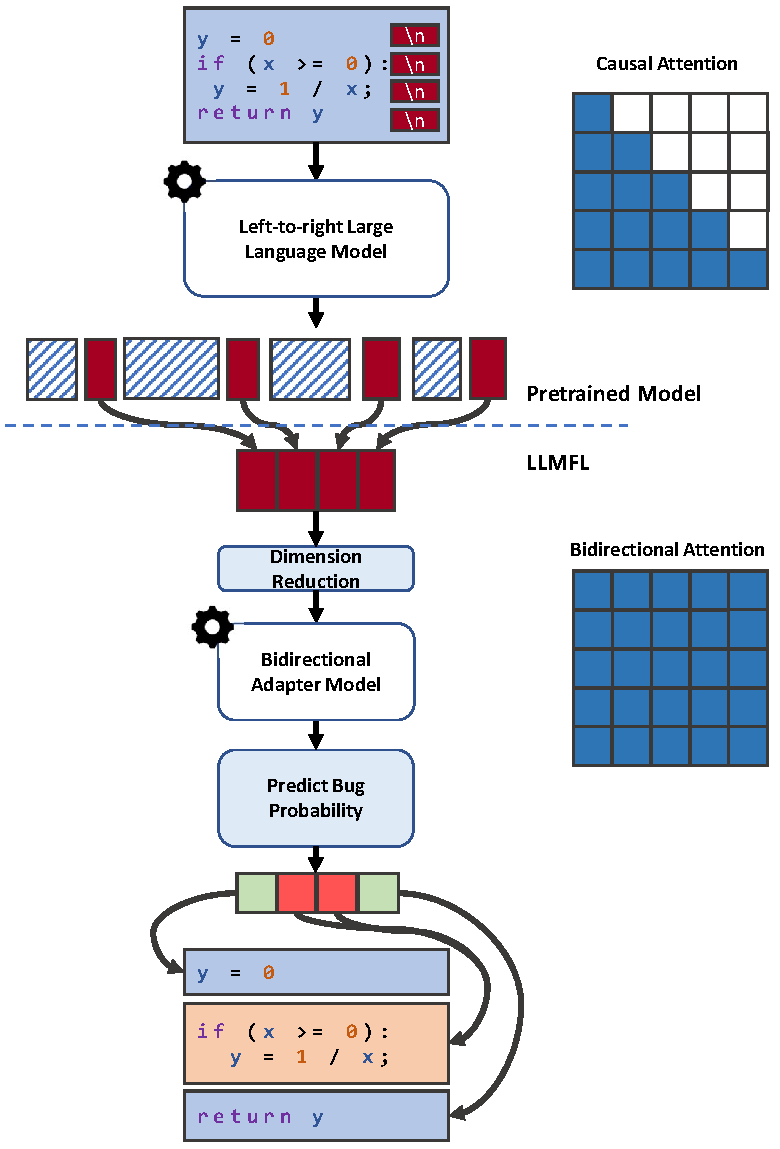
\includegraphics[width=0.6\textwidth]{figures/approach/attention.pdf}
%\vspace*{-3mm}
\caption{\small Attention masking procedure of \textit{LLMAO}}
\label{fig:attention}
\end{figure}

\subsection{Bidirectional Adapter}
\label{sec:adapter}
While left-to-right language models extract rich representations per token, they are ill-suited for fault prediction because the representation of each given token only reflects knowledge of its left-ward context. One solution might predict buggy lines based on the final hidden state, reflecting the model's knowledge after the entire file has been processed, but this creates a bottleneck where that state must store information from each line in the entire file. This bottle-necking phenomenon~\cite{bengio1994learning} is precisely why the NLP field moved away from Recurrent Neural Networks, which represent sequences with a single hidden state, and towards attention-based models, which preserve and use the state of each token~\cite{vaswani2017attention}.

I postulate that I can leverage these rich learned representations at each token by training just a few more Transformer layers that allow the model to exchange information between representations of later and earlier lines, thereby generating a new, bidirectionally aware representation for each line of code. We can do so by removing the causal attention mask that normally prevents the exchange of information with ``future'' tokens in our added layers. In our case, we assume that the entire file has already been written, so this constraint is unnecessary.
This yields a \textit{bidirectional} encoder. As shown in Figure \ref{fig:attention}, the attention masking matrix for the bidirectional model allows all tokens in the sequence to attend to each other (visualized in blue).
I thus train a bidirectional adapter consisting of a configurable number of Transformer layers, following the standard Transformer encoder architecture~\cite{vaswani2017attention}. Concretely, our approach involves five steps, visualized in Figure \ref{fig:attention}:

\textbf{Step 1:} I start with a series of code tokens $C = [c_0, c_1, \ldots, c_N]$. We query a causally pretrained Transformer $\mathcal{T}_{PT}$ to transform these into a representational ``states'' $S \in \mathbb{R}^{N \times D}$, where $D$ represents the pretrained model's dimensionality. This step takes place ``offline'', as I do not tune the pretrained model. 

\textbf{Step 2:} I extract the representations of each newline token to obtain state per line in the original program: $S_{NL} \in \mathbb{R}^{M \times D} = S[c_i=\text{\textbackslash n}]$, where $M$ is the number of original newlines and typically $M \ll N$. We conjecture that these tokens' states reasonably accurately capture the information of their line in the file's prefix context.

\textbf{Step 3:} The dimension of the pretrained model's states, $D$, ranges up to 6,144 for the CodeGen models I built on. We use a significantly smaller dimension $d \ll D$ for our adapter layers, because they are trained on limited data. We first reduce the dimension of $S_{NL}$ to $R_{NL} \in \mathbb{R}^{M \times d} = S_{NL} ~ W_d$ where $W_d \in \mathbb{R}^{D \times d}$ is a learnable weight, equivalent to a fully connected layer. We experiment with dimensions $d \in \{256, 512, 1024\}$

\textbf{Step 4:} I then train an $n$-layer bidirectional Transformer adapter $\mathcal{T}_{A}$ with the same internal dimension $d$. This gives us the final representation of each newline token $A_{NL} \in \mathbb{R}^{M \times d}$, which aims to capture their role in the bidirectional context. We set the number of Transformer layers to $n = 2$.

\textbf{Step 5:} I transform each newline token's representation to a single value ranging from 0 to 1 via a sigmoid-activated dense projection $B = \sigma(R_{NL} ~ W_b)$ where $W_b \in \mathbb{R}^{d \times 1}$. The resulting predictions per newline token can be seen as probability estimates of each line being buggy according to the model. These are compared against the ground-truth labels $T \in \{0, 1\}^M$ using the binary cross-entropy loss $\mathcal{L}_{CE} = T \ln{B} + (1 - T) \ln{(1-B)}$. This loss is back-propagated through all layers up to, but not including, those in the pretrained network to obtain gradients. Given these gradients averaged across a sufficiently large mini-batch of samples, the model states are updated to make its predictions more likely to agree with the training labels.

\section{Evaluation and Results}
\subsection{Dataset}
our work investigates the effectiveness of LLMs in the setting of fault detection. 
To determine how well our proposed technique can perform on real world faults, we select datasets with source code and corresponding labeled fault lines. 
\begin{itemize}
\item{\textbf{\textit{Defects4J} V1.2.0 }:  A Java benchmark dataset with 395 bugs from 6 Java projects~\cite{just2014defects4j}.} 
I use V1.2.0 for most of our benchmarks instead of the latest version (V2.0.0) to compare on the same dataset as most prior FL techniques.
\item{\textbf{\textit{Defects4J} V2.0.0}:  A Java benchmark dataset with additional bugs over \textit{Defects4J} V1.2.0~\cite{just2014defects4j}.} To show that our approach can generalize to faults from unseen projects, we further evaluate our tool as trained on \textit{Defects4J} V1.2.0 on 226 new bugs from the newest \textit{Defects4J} version (from projects totaling 165k more lines of code). We exclude the first 45 bugs in Jsoup and all in Gson/Jacksoncore because of trouble reproducing them (as seen in prior work~\cite{lou2021boosting}).
\item{\textbf{\textit{BugsInPy}}: a Python benchmark with 493 bugs from 17 different projects~\cite{widyasari2020bugsinpy}.}
\item{\textbf{\textit{Devign}:} a C benchmark with 5,260 from two open-source projects~\cite{zhou2019devign}. The original Devign dataset contains 15,512 security vulnerabilities from four different projects~\cite{zhou2019devign}. However, the authors of Devign only released a partial dataset available online.} 



\end{itemize}
\looseness-1
All datasets include fixing commits that correspond to each fault.  I identify faulty statements as those that are changed in the git diff associated with each commit, following prior approaches~\cite{meng2022improving,ray2016naturalness,li2019oopsla}.
I then track line numbers of changed statements as training labels.

\subsection{Baselines}
    \textit{LLMAO} takes as input source code, and outputs a ranked list of probabilities corresponding to how likely a code line is buggy. To the best of our knowledge, no existing FL approaches take as input only the source code as natural language. However, we compare against existing FL approaches that take as input both source code and test code to observe if a LLM-enabled FL technique can produce comparable results without the dependence on tests or test coverage information.
    
    our baselines are recent, state-of-the-art statement-level MLFL approaches: DeepFL~\cite{li2019deepfl}, DeepRL4FL~\cite{li2021fault}, and TRANSFER-FL~\cite{meng2022improving}. DeepFL, and DeepRL4FL are MLFL techniques that take the test coverage information as model input. TRANSFER-FL builds on previous test-based MLFL approaches with pretrained information from open-source Java programs. 
    %
    I also include Ochiai~\cite{abreu2006evaluation}, the best-performing SBFL approach.  I use the prior techniques' replication packages to compute Top-N scores, including their handling of tied ranks (if any); I follow DeepFL's approach for accounting for tied ranks for Ochiai.  
    
    our tool produces a fault probability score for each line of a code file (i.e., statement level fault localization). Previous approaches output a ranked list of either suspicious statements or suspicious methods. In particular, DeepFL~\cite{li2019deepfl} is trained at the method level, i.e., predicting which methods are defective. 
    
    To compare, we follow other prior work and use DeepFL’s spectrum and mutation-based features that are applicable to detecting faulty statements.  DeepRL4FL, and TRANSFER-FL perform statement-level fault localization by default, similar to \textit{LLMAO}.
    Since the repository and processed dataset for DeepRL4FL are not publicly available, we directly cite the experimental results reported in their paper~\cite{li2021fault}. For each of the other compared techniques, we run their tool for a total time of 30 minutes, which is comparable to our tool's training time for 300 epochs.
    
    \subsection{Validation}
    For each of our three datasets, we perform a 10-fold cross validation on the entire dataset. Specifically, we shuffle the dataset and train 10 models with 90\% of the training set each, holding out the remaining 10\% for validation, so that each sample in the dataset is held out exactly once.
    This is by contrast with some prior evaluations that in their default settings, validate tools within individual projects (using one bug in a given \textit{Defects4J} project for validation and training on other bugs in that same project)~\cite{li2019deepfl,lou2021boosting, li2021fault, meng2022improving}.
    An effective and robust FL tool using machine learning or language models should be able to predict faulty locations while trained on code from different projects. 
    
    Training FL models on a particular project may produce over-fitting to a particular project and reduces applicability, requiring a relatively rich project and bug history before a technique can be used.  I therefore believe that our 10-fold validation approach is more generalizable for training models on larger code datasets. 
    As is done in some prior evaluations~\cite{li2019deepfl,li2021fault}, we also \emph{separately} evaluate the degree to which our model trained on one set of projects generalizes to a set of projects not seen in training (without retraining for those new projects).
    
    I also deploy an early-stopping mechanism for each of our training runs. We checkpoint and record the epoch with the single highest average precision and recall score on the held-out validation dataset after every epoch. Once these scores stop improving for sufficiently many epochs (i.e., around 300 for all our model configurations), we stop training and use the best-performing checkpoint to calculate the Top-N metrics against the ground-truth labels.
    
    \subsection{Evaluation Metrics} I use the following evaluation metrics:

    
    \begin{table}[t]
    \centering
    \caption{\small Hyperparameters used for model training, both for the model trained from scratch and the three models trained on top of the various \textit{CodeGen} models}
    \begin{tabular}{l|rrrr}
    \toprule
    \textbf{Hyperparameter} & \textbf{From Scratch} & \textbf{350M} & \textbf{6B} & \textbf{16B}\\
    \midrule
    Max learning rate  &  5e-6 & 1e-4 & 7e-6 & 4e-6\\
    Min learning rate  &  1e-8 & 1e-7 & 1e-7 & 1e-7\\
    Model dimension & 256 & 1024 & 4096 & 6144\\
    Layers  &  8 & 2 & 2 & 2\\
    Batch size & 64 & 32 & 32 & 32\\
    Epochs & 2000 & 300 & 300 & 300\\
    \bottomrule
    \end{tabular}
    \label{table:hyperparams}
    \end{table}
    
    \begin{table*}[t]
    \centering
    \caption{\small \textit{LLMAO} performance on 395 bugs from \textit{Defects4J} V1.2.0, compared to prior techniques (top); on 226 additional bugs from \textit{Defects4J} V2.0.0 (middle); and with ablation (bottom, again on defects from \textit{Defects4J} V1.2.0)}
    \begin{tabular}{p{1.9cm}|lrrr}
    \toprule
     \textbf{FL type} & \textbf{Technique} & \textbf{Top-1} & \textbf{Top-3} & \textbf{Top-5}   \\
    \midrule
    \multirow{1}{*}{SBFL}
    & Ochiai              & 19 (4.8\%) & 65  (16.5\%) & 99 (25.1\%)  \\
    \midrule
    \multirow{4}{*}{MLFL}
    & DeepFL             & 57 (14.4\%) & 95 (24.1\%) & 135 (34.2\%) \\
    & DeepRL4FL          & 71 (18.0\%) & 128 (32.4\%) & 142 (35.9\%) \\
    & TRANSFER-FL        & 86 (21.8\%) & 135 (34.2\%) & 160 (40.5\%) \\
    \midrule
    \multirow{2}{*}{LMFL}
    & \textit{LLMAO} with \textit{CodeGen}-350M     & 82 (20.8\%) & 106 (26.8\%) & 126 (31.9\%) \\
    & \textit{LLMAO} with \textit{CodeGen}-6B        & 85 (21.5\%) & 115 (29.1\%) & 160 (40.5\%)\\
    & \textit{LLMAO} with \textit{CodeGen}-16B       & \textbf{88 (22.3\%)} & \textbf{149 (37.7\%)} & \textbf{183 (46.3\%)} \\
    \midrule\midrule
    LMFL, new projects & \textit{LLMAO} with \textit{CodeGen}-16B & 72 (31.9\%) & 93 (41.2\%) & 123(54.4\%) \\
    \midrule\midrule 
    \multirow{2}{*}{Ablation}
    & \multicolumn{1}{p{5cm}}{\raggedright $-pretraining$ \\ 
    \raggedright (6 layers, trained from scratch)}
    & 5 (1.3\%)   & 24 (6.2\%) &  30 (7.6\%)\\
    & \multicolumn{1}{p{5cm}}{\raggedright $-bidirectional~adapter$ \\ 
    \raggedright (predict directly from \textit{CodeGen}-16B)} & 10 (2.6\%)   & 60 (15.2\%) &  85 (21.5\%)\\
    \bottomrule
    \end{tabular}
    \label{table:topn}
    \end{table*}
    
    \paragraph{Top-N.}
    Top-N measures the number of faults with at least one faulty
    element located within the first N positions (N=1, 3, 5). Developers only examine a small amount of the most-likely buggy elements within a ranked list~\cite{parnin2011automated}, with particular attention paid to the top-5 elements~\cite{kochhar2016practitioners}. To compare against state-of-the-art techniques, we adopt Top-N following prior work~\cite{li2022fault, li2019deepfl, lou2021boosting}.
    
    \vspace{-0.5em}
    \paragraph{AUC of the model's ROC Curve.}
    Although most developers inspect only top-5 elements in a given list, we also aim to measure how overall prediction compares against the ground truth.
    A Receiver Operating Characteristic (ROC) curve shows the performance of one classification model at all thresholds. It can be used to evaluate the overall model strength for making precise and accurate predictions. The area under an ROC curve (AUC) measures the usefulness of a test. AUC is a number between 0 and 1; higher is better.  I measure the AUC at each of our model's top performing points in time, averaging precision and recall. We choose AUC to observe the prediction strength of our models at their peak performance. 
    
    \subsection{Ablations}
    I conduct an ablation analysis to evaluate the impact of different components on the performance of our model (RQ3). 
    I run five variants of our proposed technique for the \textit{Defects4J} V1.2.0 dataset.
    I first evaluate \textit{LLMAO} pretrained on \textit{CodeGen}, and \textit{LLMAO} without any pretraining to evaluate the impact of the pretrained large language model's final hidden states.
    For the pretrained models, we checkpoint with three different \textit{CodeGen} sizes (i.e., 350 million, 6 billion, and 16 billion parameters) to evaluate the impact of the pretrained model's size on finetuning. 
    I also train a version of our model without bidirectional layers, using only the \textit{CodeGen} auto-regressive attention mechanisms for fault localization. We aim to determine if left-to-right LLMs can detect faults directly, without any customization for code understanding. 
    
    
    \subsection{Hyperparameters}
    \label{sec:hyperparameters}
    Table \ref{table:hyperparams} shows the hyperparameters used in training all our models.
    I reduced the learning rates until both the training and validation loss converged in a stable manner. Following the established practice in language model training \cite{hoffmann2022training}, we use a learning rate warm-up of 1000 steps and a cosine learning rate decay until a global minimum learning rate of 1e-7 across 20k steps.
    Each model is trained on a single GPU. For the \textit{CodeGen} pretrained models, we use a uniform batch size of 32 and perform gradient accumulation to ensure every batch of our data fits on a single GPU.
    For a fair comparison of \textit{LLMAO}'s components (RQ3), we use the same number of  training epochs (300) for all pretrain sizes and projected dimensions. However, the non-pretrained bidirectional model requires a much longer training time (some 2,000 epochs) for the validation loss to converge.
    
    I train all configurations of our model on a uniform dimension of 512, which is projected down from the various \textit{CodeGen} models' hidden state dimensions (i.e., 1024, 4096, and 6144). We use a 8 attention heads for all our models.
    
    
    \subsection{Results}
    \textbf{RQ1: How does \textit{LLMAO} compare with prior DL-based FL tools?}
    Table \ref{table:topn} (top) details experimental results showing how our tool compares against state-of-the-art FL techniques. The first 4 techniques are from prior approaches; I evaluate our \textit{LLMAO} using three \textit{CodeGen} pretrain sizes. The results show the Top-N (N $\in \{1,3,5\}$) score for each technique. 
    Table \ref{table:topn} shows that \textit{LLMAO} with the largest (16B) pretrained \textit{CodeGen} size outperforms all the compared techniques. Even with smaller pretrain sizes (350M and 6B), \textit{LLMAO} performs similarly to the top-performing prior methods.
    
    Per Table \ref{table:topn}, \textit{LLMAO} with 16B \textit{CodeGen} pretrain size detects 84 more faults within Top-5 than the top-performing SBFL technique, Ochiai (84.8\% improvement). \textit{LLMAO} detects 48 more faults within the Top-5 than the first proposed deep learning based FL technique DeepFL (35.6\% improvement), and 23 more faults within the Top-5 than the latest state-of-the-art test-based MLFL approach TRANSFER-FL (14.4\% improvement). 
    For the Top-3 and Top-1 metric, \textit{LLMAO} pretrained on the 16B \textit{CodeGen} model can detect 14 more faults (10.4\% improvement) and 2 more faults (2.3\% improvement) than the state-of-the-art tool TRANSFER-FL. We observe that our LMFL technique improves particularly over prior FL techniques when more suspicious lines are inspected (i.e., higher Top-5 scores). 
    
    A Wilcoxon signed-rank test~\cite{woolson2007wilcoxon} indicates that the top-N values the difference between \textit{LLMAO} with \textit{CodeGen}-16B and prior techniques in terms of performance at the several top-N values is statistically significant (p-values ranging from 0.01 to 0.03).
    
    When considering Top-1 scores, our approach is only slightly better than TRANSFER-FL, which performs roughly on-par with our \textit{CodeGen}-6B model. 
    However, note that prior techniques only achieve comparable results with our tool by requiring readily-available tests and test coverage as input. Writing tests and producing test coverage are time-consuming activities, and tests are not always available or useful when debugging. Furthermore, both DeepFL and TRANSFER-FL techniques include mutation-based fault localization information, which is very time-consuming to collect (i.e., hours of online collection time per bug~\cite{li2019deepfl}).
    
    
    \begin{tcolorbox}
    [colback=white,colframe=black,arc=0pt,boxrule=0.5pt,title=RQ1 Summary,boxsep=2pt,left=1pt,right=1pt,top=1pt,bottom=1pt,fonttitle=\bfseries]
    \textit{LLMAO} pretrained on the largest \textit{CodeGen} size improves on the state-of-the-art by 14.4\% on Top-5, without relying on test cases, program analysis, or even compilable code.
    \end{tcolorbox}
    
    \vspace{0.5em}
    \noindent\textbf{RQ2. How well does \textit{LLMAO}’s performance generalize to new
    projects?}
    %
    I additionally evaluate \textit{LLMAO} on bugs from the newer \textit{Defects4J} V2.0.0, on projects that were not seen in pretraining (an additional 165K lines of code). The ``LMFL, new projects'' row in Table~\ref{table:topn} shows that \textit{LLMAO} with 16B \textit{CodeGen} pretrain size detects 72/226 faults in top 1, 93/226 faults in top 3, and 123/226 faults in top 5. 
    
    Although I avoid strong statistical claims in this case study setting, these results are comparable to \textit{LLMAO}'s performance on projects included in its training data, suggesting that it generalizes well.  Several previously-published techniques are also evaluated for cross-project generalizability, in a variety of experimental settings.  DeepFL and DeepRL4FL repeatedly train a model on N-1 projects and test it on a held-out project; in both cases, performance on the cross-project setting degrades compared to the within-project setting.  GRACE~\cite{lou2021boosting} localizes to the method level (rather than the statement level); its cross-project evaluation also looks at defects from \textit{Defects4J} V2.0.0.  GRACE's performance also degrades slightly on  new defects, though less than prior work.  A key advantage of our approach is that \textit{LLMAO} generalizes well to unseen projects \emph{without retraining of any kind}.  This argues for our technique's practicality both in terms of performance and time/compute requirements.  
    
    \begin{tcolorbox}
    [colback=white,colframe=black,arc=0pt,boxrule=0.5pt,title=RQ2 Summary,boxsep=2pt,left=1pt,right=1pt,top=1pt,bottom=1pt,fonttitle=\bfseries]
    \textit{LLMAO} pretrained on the largest \textit{CodeGen} size using data from \textit{Defects4J} V1.2.0 performs well on bugs in unseen projects (not included in the training data), without additional training costs.
    \vspace{0.5em}
    \end{tcolorbox}
    
    \begin{table}[t]
    \centering
    \caption{\textit{LLMAO}'s Top-N Effectiveness on Different Datasets}
    \begin{tabular}{l|rrr}
    \toprule
    \textbf{Metric} &\textbf{\textit{BugsInPy}} & \textbf{\textit{Defects4J}} & \textbf{\textit{Devign}}\\
    \midrule
    \# lines  &  76,672 & 168,960 & 7,180,160\\
    Top-1  &  51/493 (10.3\%) & 88/395 (22.3\%) & 1478/5260 (28.1\%)\\
    Top-3  &  59/493 (12.0\%) & 149/395 (37.7\%)  & 2050/5260 (39.0\%)\\
    Top-5  &  75/493 (15.2\%) & 183/395 (46.3\%)  & 3171/5260 (60.3\%)\\
    \bottomrule
    \end{tabular}
    %\vspace{-0.33cm}
    \label{table:topn-rq4}
    \end{table}
    
    \noindent\textbf{RQ3. How does each component of \textit{LLMAO}\ impact its performance?} 
    The bottom two rows of Table \ref{table:topn} show the impact of pretrained models on \textit{LLMAO}'s performance. 
    
    \vspace{0.5ex}
    \emph{Without Pretraining} We trained our bidirectional language model from scratch, using the same tokenizer as \textit{CodeGen} for tokenizing the inputs. We replace \textit{CodeGen}'s token-level representation with a learnable embedding for each token. We then pass these embeddings through 6 bidirectional Transformer layers (a typical minimum for Transformers) and predict the bugginess probability for states corresponding to newline tokens only (other tokens are embedded alongside these but ignored in the final layer). This model, trained on a sample size of 395 (i.e., total number of labeled \textit{Defects4J} bugs) can achieve only a Top-1 of 5 (1.3\%), Top-3 of 24 (6.2\%), and Top-5 of 30 (7.6\%). \textit{LLMAO} without any pretraining performs significantly worse than \textit{LLMAO} based on any size of \textit{CodeGen}. 
    
    \vspace{0.5ex}
    \emph{Without the Bidirectional Adapter} I train a single linear projection from \textit{CodeGen}-16B's final hidden states to a bugginess score for each line, thus omitting the bidirectional attention adapter layers. This approach performs better than \textit{LLMAO} trained from scratch, with a Top-1 of 10 (2.6\%), Top-3 of 60 (15.2\%), and Top-5 of 85 (21.5\%). This highlights how much program understanding a left-to-right LLM trained on a large corpus of code encodes in its learned representations. Although left-to-right models are not targeted at text-understanding, a LLM that can generate code given a natural language prompt can evidently learn to understand faults to a similar level of top performing SBFL approaches. Given enough fine-tune training on top of the previous task of code generation, CodeGen-16B without any further configuration is able to detect 85 \textit{Defects4J} bugs (21.5\%), which is only 14\% worse than the top performing SBFL model Ochiai. However, using \textit{CodeGen}-16B for fault localization directly still performs significantly lower than all \textit{LLMAO} models with bidirectional adapter layers.
    I perform an additional Wilcoxon signed-rank test~\cite{woolson2007wilcoxon} to observe that the top-N values of \textit{LLMAO} with \textit{CodeGen}-16B yields significantly better results than \textit{LLMAO} without pretraining and without the bidirectional adapter at $\alpha=0.05$ (p-values of 0.008 and 0.02).
    
    \vspace{0.5ex}
    \emph{Underlying LLMs}
    Comparing our tool on different pretrained \textit{CodeGen} sizes, we see an improvement in fault detection as the underlying model grows.
    \textit{LLMAO} pretrained on \textit{CodeGen}-350M improves upon \textit{LLMAO} without the bidirectional adapter layers by 72 on Top-1. \textit{LLMAO} pretrained on \textit{CodeGen}-6B can detect 3 more faults on Top-1 than \textit{CodeGen}-350M, and \textit{LLMAO} pretrained on \textit{CodeGen}-16B can find an additional 3 compared to \textit{CodeGen}-6B.
    At higher Top-N targets, the performance improves more steeply with the size of the underlying model. For instance, \textit{LLMAO} fine-tuned on \textit{CodeGen}-350M detects 96 more faults than without pretraining, while fine-tuning on top of \textit{CodeGen}-16B uncovers another 153.
    

\begin{figure}
\centering
     \begin{subfigure}{}
         \centering
         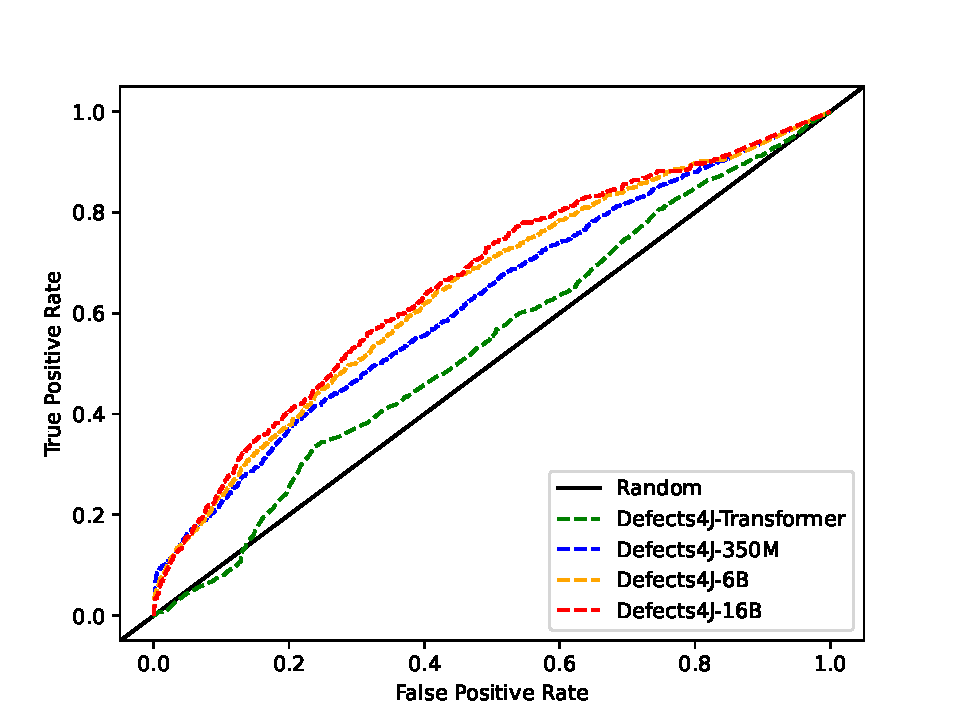
\includegraphics[width=7cm]{figures/roc/defects4j_roc.pdf}
         \caption{ROC curves on the \textit{Defects4J} dataset}
         \label{roc:defects4j}
     \end{subfigure}
     \begin{subfigure}{}
         \centering
         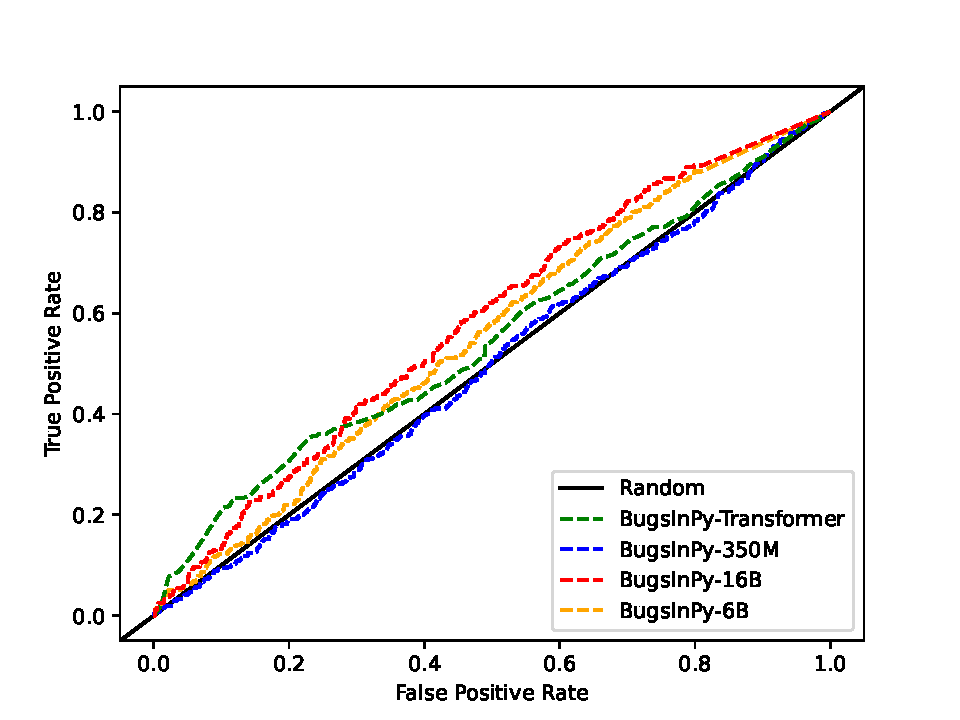
\includegraphics[width=7cm]{figures/roc/bugsinpy_roc.pdf}
         \caption{ROC curves on the \textit{BugsInPy} dataset}
         \label{roc:bugsinpy}
     \end{subfigure}
     \begin{subfigure}{}
         \centering
         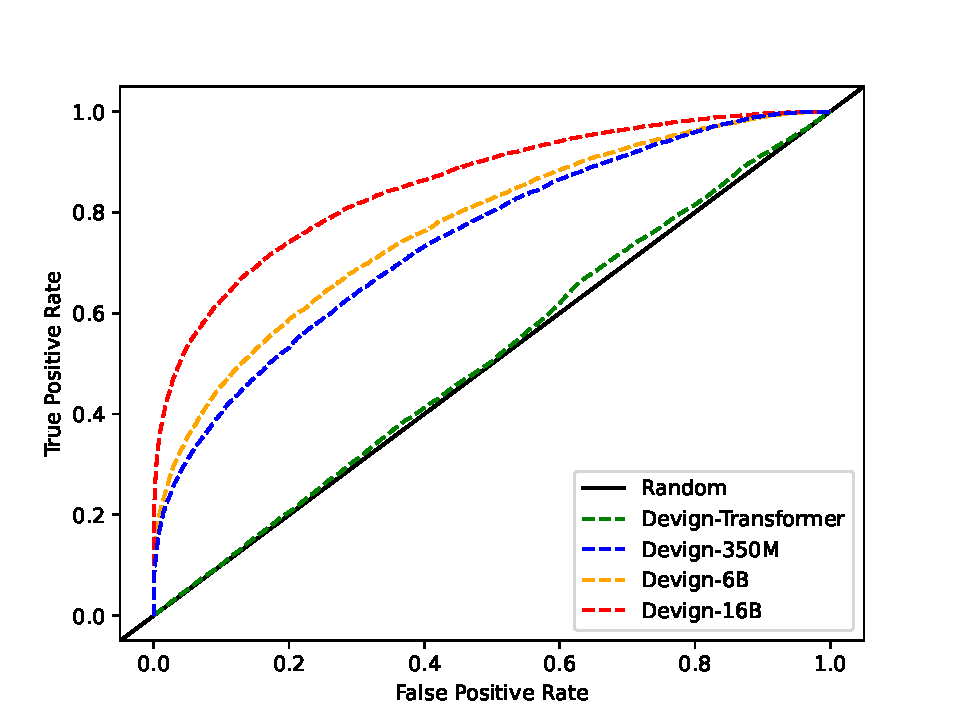
\includegraphics[width=7cm]{figures/roc/devign_roc.pdf}
         \caption{ROC curves on the \textit{Devign} dataset}
         \label{roc:devign}
     \end{subfigure}
\label{fig:roc}
\vspace{-2mm}
\caption{ROC curves on the completely random prediction, our model without any pretraining (Transformer), and pretrained on \textit{CodeGen}-small (350M), \textit{CodeGen}-medium (6B), and \textit{CodeGen}-large (16B). Higher area under the curve (AUC) represents stronger predictive power.}
\end{figure}

\begin{tcolorbox}
[colback=white,colframe=black,arc=0pt,boxrule=0.5pt,title=RQ3 Summary,boxsep=2pt,left=1pt,right=1pt,top=1pt,bottom=1pt,fonttitle=\bfseries]
Although left-to-right language models can directly localize some faults, adding the bidirectional adapter layers is crucial for achieving state-of-the-art fault localization. Furthermore, we show that our tool using the largest pretrained LLM (i.e., \textit{CodeGen} 16B) significantly outperforms all other variations of our model.
\vspace{0.5em}
\end{tcolorbox}

\noindent\textbf{RQ4. How generalizable is \textit{LLMAO} to other languages and domains?}
To evaluate our proposed technique on different languages and domains, we run all three pretrain sizes of our tool on the \textit{BugsInPy}~\cite{widyasari2020bugsinpy} dataset for localizing Python bugs, and the \textit{Devign}~\cite{zhou2019devign} dataset for localizing C security vulnerabilities. We believe that measuring our tool on two other languages and one other defect domain can evaluate the effectiveness of modeling code defects as specific behaviors in natural language. 

 I observe from Table \ref{table:topn-rq4} that \textit{LLMAO} can localize faulty statements with Top-1 of 10.3\% on \textit{BugsInPy}, and 28.1\% for \textit{Devign}. 
I observe that the performance of \textit{LLMAO} improves as the size of the training dataset increases. Although \textit{Defects4J} has fewer bugs than \textit{BugsInPy}, we find that in total, \textit{Defects4J} has 53\% more code lines combined from all code files than the \textit{BugsInPy} dataset. Since our approach considers source code as natural language, a larger database of code lines gives our models more training data. In particular, our largest dataset \textit{Devign} with over 7 million lines of code achieves a Top-5 of 60.3\% (i.e., 60.3\% of our model's top-5 suspicious lines have at least one line that is an actual vulnerability). 
    
Figures \ref{roc:defects4j}, \ref{roc:bugsinpy} and \ref{roc:devign} show the ROC curve for each of our trained models compared to the completely random curve (i.e., AUC=0.5).
A ROC curve shows the performance of our model at all classification thresholds. 
The completely random curve has the true positive rate equal to the false positive rate at every classification threshold.
I plot the ROC for our model trained on \textit{Defects4J}, \textit{BugsInPy}, and \textit{Devign} after 300 epochs without any pretraining (i.e., the Transformer ROC curve), \textit{CodeGen}-350M pretraining, \textit{CodeGen}-6B pretraining, and finally \textit{CodeGen}-16B pretraining. 

I observe a clear improvement on the AUC as I use the \textit{CodeGen} final hidden states for training, and the AUC continues to improve as I use larger \textit{CodeGen} models. 
In particular, the AUC for Figure \ref{roc:defects4j} yields 0.539 on \textit{Defects4J} trained from scratch, 0.573 on \textit{Defects4J} trained from \textit{CodeGen}-350M, 0.638 on \textit{Defects4J} trained from \textit{CodeGen}-6B, and 0.677 on \textit{Defects4J} trained from \textit{CodeGen}-16B.
Figures \ref{roc:bugsinpy} and \ref{roc:devign} show a significant improvement in our model's predictive power as I use a larger dataset of code corpus. \textit{LLMAO} with \textit{CodeGen}-16B trained on our smallest dataset \textit{BugsInPy} yields an AUC of 0.571, and \textit{LLMAO} with \textit{CodeGen}-16B trained on our largest dataset \textit{Devign} yields an AUC 0.855. We observe that our model's predictive performance on \textit{Devign} is better than our model's predictive performance on \textit{BugsInPy} at all thresholds.

    \begin{tcolorbox}
    [colback=white,colframe=black,arc=0pt,boxrule=0.5pt,title=RQ4 Summary,boxsep=2pt,left=1pt,right=1pt,top=1pt,bottom=1pt,fonttitle=\bfseries]
    \textit{LLMAO} is more confident in its fault detection as the size of both training data and the pretrained model scale up. \textit{LLMAO} is also particularly effective for locating security bugs in C where test cases are not available.

    \vspace{0.5em}
    \end{tcolorbox}

\section{Conclusion}
\label{sec:LLMAO-conclusion}
As a first step in using LLMs for maintaining software evolution, we propose bidirectional adapter fine-tuning for localizing program defects, which include general logic defects as well as security vulnerabilities. We perform an empirical study on 395 real bugs from \textit{Defects4J}, 493 bugs from \textit{BugsinPy}, and 5,260 security vulnerabilities from \textit{Devign}. The results show that our technique can outperform existing state-of-the-art deep learning based fault localization techniques without the dependency on any test cases.

\chapter{Automated Program Repair}
\label{ch:entropy}
Automated Program Repair (APR) aims to help software engineers automatically patch software bugs. Although LLMs can immediately be used as code generators, it remains unclear how LLMs can be used as bug patchers.
In this chapter, we argue that LLMs can be powerful tools for APR when combined with prior traditional APR techniques. When used correctly, LLMs can save both software testing time and manual patch selection time.

LLMs are trained on large volumes of code in which defects are relatively
rare. Since their training objective encourages next-token prediction,
well-trained language models tend to simultaneously perceive faulty code as unlikely
(or ``unnatural'') and to produce code that is correct, as correct code is more
``natural''~\cite{NAT}. The naturalness of code and unnaturalness of buggy 
code is now a well-established phenomenon~\cite{hindle2016naturalness,NAT}.
However, the bulk of prior research on this topic relied on relatively simple $n$-gram language
models~\cite{ngram}. Compared to present-day LLMs, these models provided a
very poor estimator of code predictability. The ``unnaturalness'' of
buggy lines was therefore mainly useful as an explanatory metric, but showed limited
utility for precisely localizing defects, let alone repairing programs.
The recent advancement of much larger and more sophisticated LLMs have decreased model
perplexities by multiple orders of magnitude. This makes them a much more accurate adjunct both for estimating naturalness and
for fault localization or correct patch identification~\cite{xia2023automated,
yang2023large}.

We revisit the idea of naturalness for program repair. 
LLMs can only go so far on their own in reasoning about and
fixing buggy code. It moreover motivates the use of traditional tools, which
compress such information, as a complement to LLMs in repair, which has indeed
shown promising recent results for the patch generation stage in
particular~\cite{xia2023automated} (acknowledging the risk of training data
leakage in any such experiment~\cite{balloccu2024leak}). 
I go beyond prior work by interrogating the role of entropy as a complement to
traditional repair at every stage:

\noindent\textbf{Plausible patch generation.} APR approaches
typically generate multiple potential code changes in search of 
\emph{plausible} patches that cause the program to pass all tests.
Executing tests (and to some extent, compiling programs to be tested) dominates
repair time: the template-based approach \textit{TBar}~\cite{TBar} spends about 2\% of
its total time creating patch templates, 6\% generating patches from templates,
and 92\% running tests on generated patches. Regardless of the patch generation method (e.g.,
symbolic techniques~\cite{patch-sim, claire_apr,angelix}, template instantiation~\cite{TBar, kim2022multi}, or
machine learning models~\cite{xia2023automated}) repair \emph{efficiency} is best
approximated in terms of the number of patches that must be evaluated to find a
(good) repair~\cite{efficiency}.
I show that entropy, when used to order candidate patches for evaluation, can
improve the efficiency of generic template-based repair by 24
tested patches per bug, on average.

\vspace{1ex} 
\noindent\textbf{Patch correctness assessment.}
Plausible patches are not always correct, in that they can fail to generalize to
the desired behavior beyond what is tested in the provided test 
suite~\cite{CURE}.  Some recent work aims to address this in the form of a 
post-processing step that identifies (and filters) plausible-but-incorrect
patches, typically by combining program analysis and machine
learning~\cite{Panther, Shibboleth, yang2023large}.  However, techniques to date
are typically trained on the same test suites used for patch generation,
imposing a project-specific training burden (and an expensive one, when dynamic
signals are required), and posing a significant risk of overfitting~\cite{CURE, yang2023large}.  
I show that entropy can rank correct patches 49\% more effectively (in Top-1) than state-of-the-art patch ranker Shibboleth~\cite{Shibboleth}, without using any project-specific training data.

\section{LLM Entropy for APR}
\begin{figure*}[t]
\centering
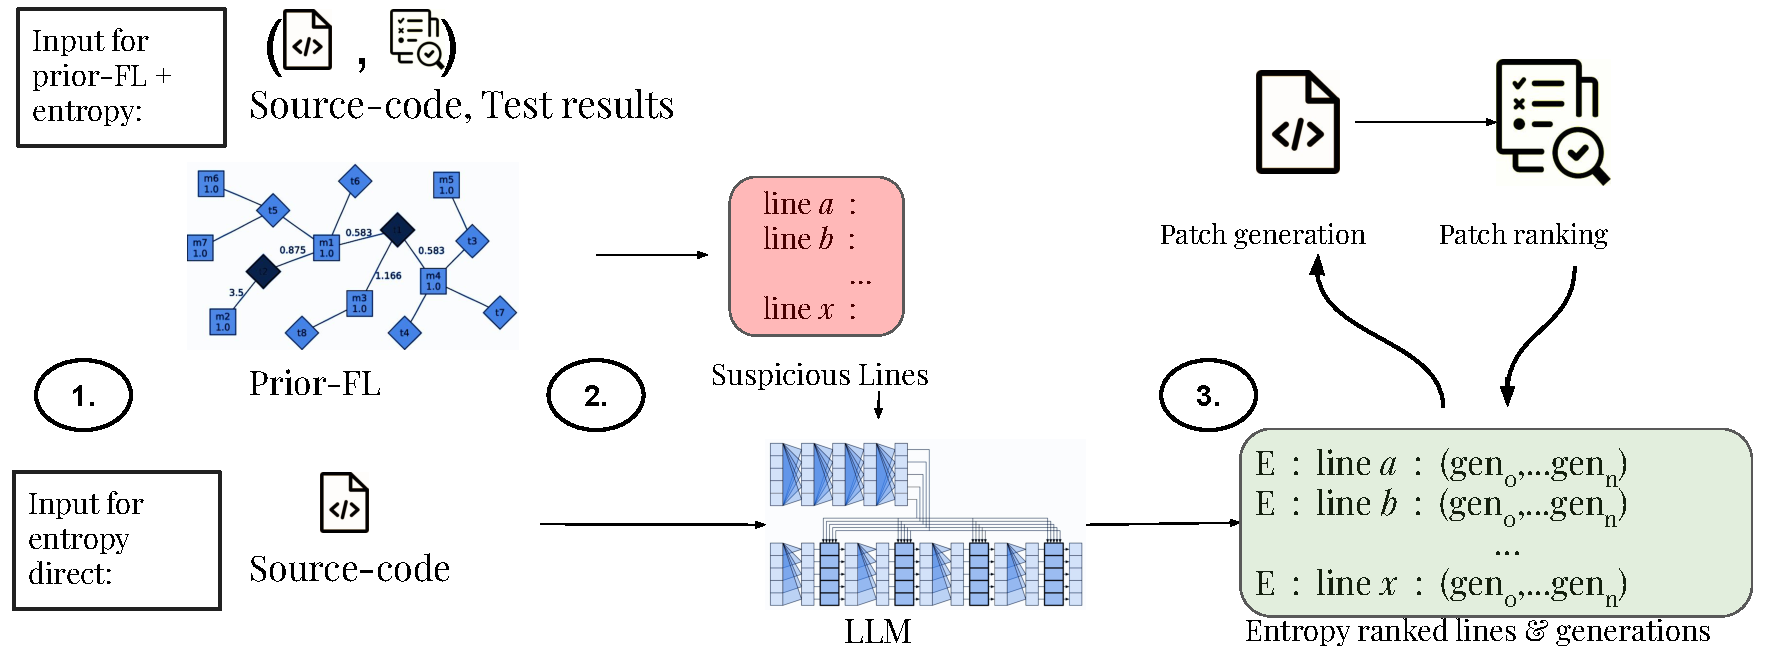
\includegraphics[width=\textwidth]{figures/approach/entropy_approach.pdf}
\caption{Fault localization pipeline using entropy. (1) I take a prior-FL suspicious score list, (2) query each code-line for entropy values, and (3) re-rank the list using LLM entropy scores.}
\label{fig:fl-method}
\end{figure*}


This section describes how I use entropy for evaluating patches; and our modifications to TBar to enable our
 study of improved patch efficiency.
I calculate entropy with the following equation:
$Entropy = -\sum_{i=1}^{n}\frac{log(p_{ti})}{n}$.

\subsection{Entropy-Delta}
\label{sec:entropy-delta}
\begin{figure}
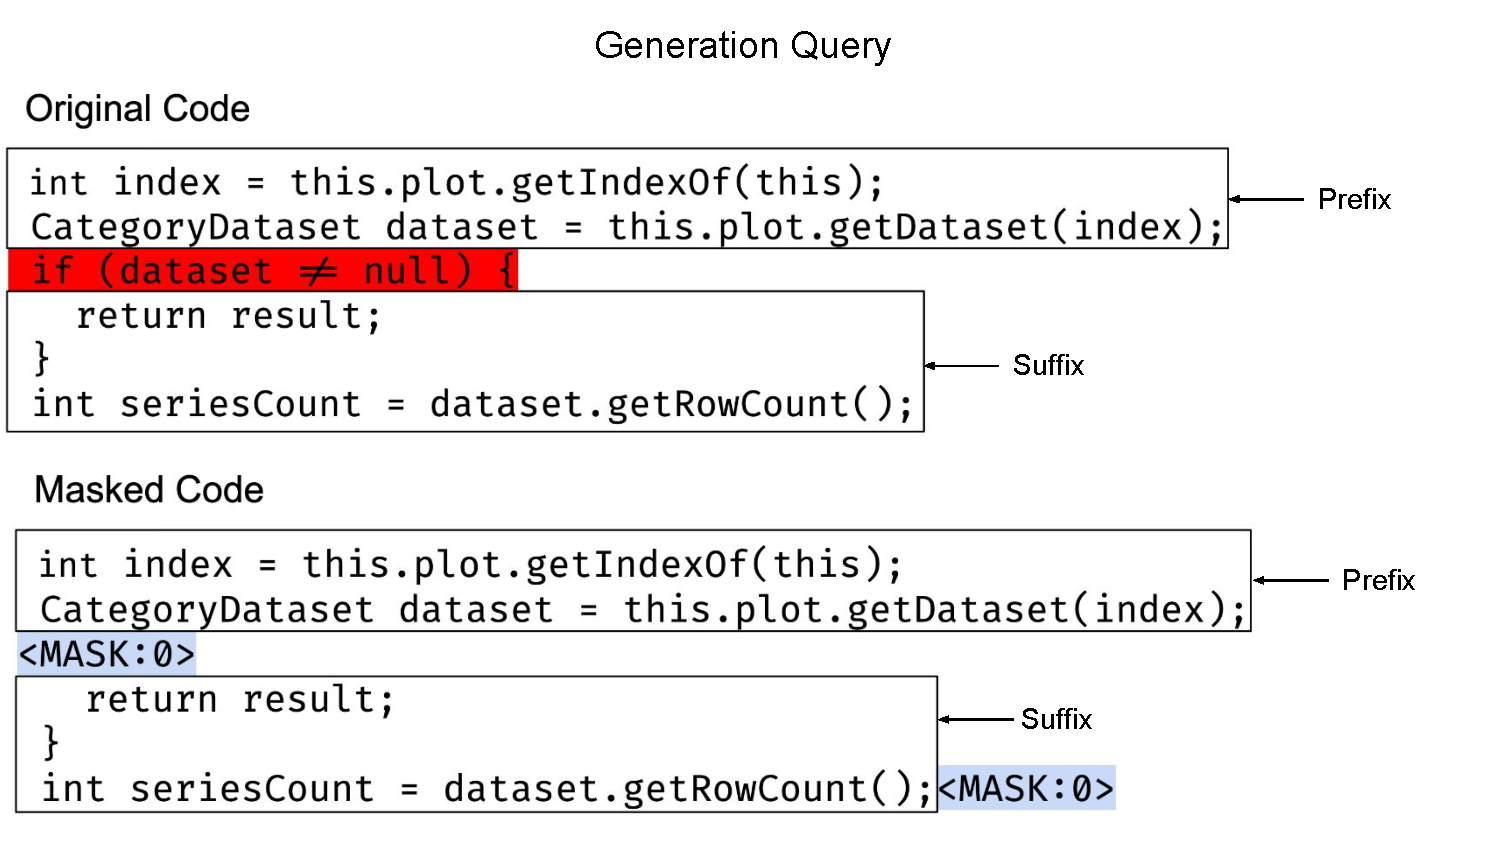
\includegraphics[width=0.7\textwidth]{figures/approach/generation_query.pdf}
\caption{An example of entropy-delta query from a code-line deletion patch. The entropy-delta value of the deleted line is the difference between the original line and a blank line.}
\label{fig:deletion-method}
\end{figure}

\begin{figure}
  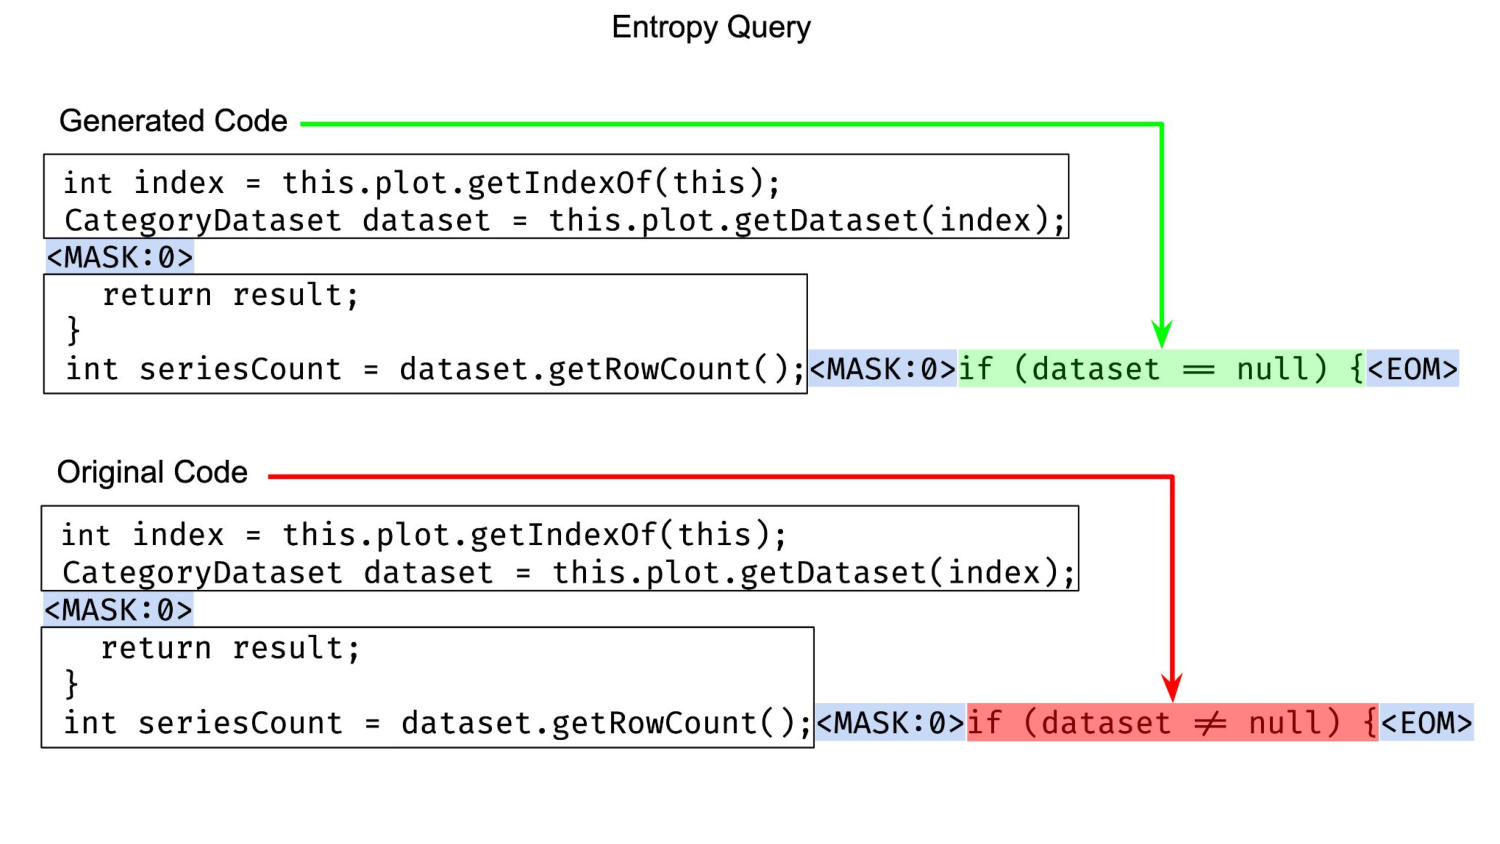
\includegraphics[width=0.7\textwidth]{figures/approach/entropy_query.pdf}
  \caption{An example of entropy-delta query from a code-line replacement patch. The entropy-delta value of the replaced line is the difference between the original line and the replacement line.}
  \label{fig:replacement-method}
\end{figure}

To evaluate patch naturalness, which I use in both patch prioritization during
generation/evaluation and patch correctness prediction, we introduce the concept of an
``entropy-delta''. Entropy delta describes how code replacement changes the naturalness
of a block of code. Figure~\ref{fig:deletion-method} and
Figure~\ref{fig:replacement-method} give examples for our usage of entropy-delta
for assigning a ranking score for patches. Figure~\ref{fig:deletion-method}
shows the process of masking out a deleted line of code and querying the LLM for
the change in entropy using that mask (i.e., the change in entropy without the original line). Figure~\ref{fig:replacement-method} shows
the process of querying the LLM for the change in entropy if the tokens of the
original line of code is replaced with new tokens of patch code. If the patch is
an insertion of a blank new line, we query the entropy-delta between the ``newline'' token and the original line of code.
For the case of an insertion, we measure the entropy-delta between the new code line and the original blank line.

An entropy-delta is simply the change in entropy before and after a line in code
is replaced. For instance, if the line's original entropy is 1.0, and the
replacement line's entropy is 0.5, then the line has an entropy-delta of +0.5,
as in, replacing that line lowered entropy by 0.5. A significant reduction in
entropy (large, positive entropy-delta) means that the replacement code lowered
the entropy, implying both that the original statement may have been buggy and
that the patch is more natural for that region of code. A large, negative
entropy-delta means that the replacement code increased entropy, meaning that
the patch is less natural at that location. An entropy-delta of 0 means that the
patch has the exact same naturalness as the original code.


\subsection{Modified TBar}
\label{sec:entropy-tbar}

our patch efficiency experiments ask how entropy can speed up patch generation
and evaluation.  I evaluate it in context of TBar~\cite{TBar}, the best-performing
template-based program repair technique in the existing literature.  I avoid
using ML-based APR techniques (even though some may outperform TBar~\cite{xia2023automated, TransferFL, Dear}) because our goal is a controlled evaluation of entropy without learned patterns from the test suite.  Evaluating based on a technique that otherwise also relies on trained ML
models fails to isolate the effect of entropy per se.

TBar is a template-based patch generation technique
integrated with Defects4J V1.2. Our experiments require several modifications to the
codebase.  First, we enable TBar to continue seeking patches after the first
test-patching patch is found.  Second, we enable TBar to generate patches, or
evaluate them in a customized order (such as one provided by an entropy-delta ranking).
our TBar extension also includes some refactoring for
modifiability/extensibility, as well as a more accurate patch caching mechanism
(caching the patched source code, rather than the patch alone).  I provide the
modified code with our replication package.


\section{Evaluation and Results}

In this section, we describe the models I use for entropy
(Section~\ref{sec:llms}), the bug and patch datasets considered
(Section~\ref{sec:dataset}), as well as evaluation metrics (Section~\ref{sec:metrics}).

\subsection{LLMs}
\label{sec:llms}

I used inCoder~\cite{inCoder}, Starcoder~\cite{Starcoder}, and Code-Llama2
\cite{Llama}. The three LLMs were trained on open-source code and are capable of
infilling with bidirectional context. The inCoder model~\cite{inCoder} is a
large-scale decoder-only Transformer model with 6.7 billion parameters. The
model was trained on a dataset of code from public open-source repositories on
GitHub and GitLab, as well as from StackOverflow. 
% The dataset includes code
% written in various programming languages, with a focus on Python and JavaScript.
%The model was also trained on code written in 28 other programming languages.
inCoder was primarily trained for code infilling, which involves the insertion
of missing code snippets in existing code, using a causal-masked objective
during training. However, its versatility enables it to be utilized in a variety
of software engineering tasks, including automatic program repair. Starcoder and
Llama-2 were trained with a similar autoregressive plus causal-mask objective as
inCoder. Starcoder was trained with 15.5 billion parameters. Code-Llama2 have
three versions available: 7B, 13B and 34B. We choose the 7B version as it is
the closest in size to the other two models. Although the three LLMs were
not specifically trained for repair, their large architectures and training
objectives could imply that their entropy values on a particular region of code
could suggest code naturalness. For all experiments, we set the LLM temperature
to 0.5.

\subsection{Dataset}
\label{sec:dataset}

\begin{table}[t]
    \centering
  \caption{\small Defects4J bugs with at least one patch passing tests (efficiency), and a developer fix (patch correctness).}
  \begin{tabular}{l|rr|rr}
  \toprule
  & \multicolumn{2}{c}{\textbf{Defects4J V1.2 \#bugs}}  & \multicolumn{2}{c}{\textbf{Defects4J V2.0 \#bugs}}  \\
  & \multicolumn{2}{c}{Patch efficiency}  & \multicolumn{2}{c}{Patch
  correctness}  \\
  & Incl. & Total & Incl. & Total \\
  \midrule
  Chart  & 11  & 26 & 19  & 26\\
  Closure  & 19 & 133&  64 & 174\\
  Lang  & 14 &65& 35 & 64\\
  Math  & 21 & 106 & 67  & 106\\
  Mockito  & 3 & 38&  1  &38\\
  Time  & 4 & 27  & 11 & 26\\
  \midrule
  Total & 72 & 395 & 197 & 434 \\
  \bottomrule
  \end{tabular}
  \label{table:datasets}
  \end{table}

I use the Defects4J~\cite{just2014defects4j} dataset as the basis of our
experiments.  Defects4J is a well-established set of documented historical bugs in Java
programs with associated tests and developer patches. It is commonly used in
APR, testing, and fault localization research. However, each research question requires a different subset of the
data. Table \ref{table:datasets} shows the number of bugs in each project that
have at least one patch passing tests (for analyzing patch efficiency) and a
developer fix (for analyzing patch correctness) along with plausible but
incorrect patches. In total, we analyze 72 bugs from Defects4J V1.2 for patch
efficiency and 197 bugs from Defects4J V2.0 for patch correctness.

I used Defects4J V1.2 for the fault localization and patch generation experiments. 
I do this because off-the-shelf TBar, as well as prior fault localization tools' replication packages, are all only compatible with Defects4J V1.2. The fault localization experiments consider all 395 bugs in Defects4J V1.2.  
I choose not to use Defects4J V2.0 for fault localization because prior tools' replication packages are only compatible with Defects4J V1.2. 

For patch generation, the goal is to evaluate the degree to which entropy can improve repair efficiency; I therefore focus on the subset of Defects4J V1.2 bugs on which vanilla TBar succeeds at least once.

For patch correctness ranking, we use curated datasets from prior tools'
replication packages directly, namely, Shibboleth~\cite{Shibboleth} and
Panther~\cite{Panther}. Shibboleth and Panther are both tools that leverage
static and dynamic heuristics from both test and source code to rank and
classify plausible patches, built on top of the updated Defects4J V2.0 dataset. We
use a dataset of 1,290 plausible patches on Defects4J V2.0 curated by Ghanbari et
al.~\cite{Shibboleth}. For patch classification, we use a dataset of 2,147
plausible patches on Defects4J V2.0 curated by Tian et al.~\cite{Panther}. The
patches from Tian et al.~\cite{Panther} were generated by seven different APR
techniques. Each bug in the dataset has one correct patch and several plausible
(i.e., test passing) but incorrect ones. We calculate the change in entropy
between the section of code in the original (buggy) file and the patched
version. Note that both datasets only contain patches in projects Chart, Closure, Lang, Math, Mockito, and Time (6/17 of Defects4J V2.0's total projects), to compare with prior work built on Defects4J V1.2. Instead of the total number of bugs 835 in Defects4J V2.0, we only consider the 434 bugs in the 6 projects included by Shibboleth~\cite{Shibboleth} and
Panther~\cite{Panther} (shown in Table \ref{table:datasets}).


\subsection{Metrics}
\label{sec:metrics}
\noindent\textbf{Patch generation efficiency.} I measure the effect of
reranking generated potential patches in terms of the number of patch
evaluations saved by doing so.  Patch evaluations are established as a
hardware- and program-independent measure for APR efficiency~\cite{efficiency},
and a proxy for compute time. 
\noindent\textbf{Patch correctness.}
For patch classification tasks, we convert entropy-delta values into binary labels. We
label patches with a positive entropy-delta as ``more natural'' (i.e., more
likely to be correct), and patches with a negative entropy-delta ``less
natural'' (i.e., less likely to be correct). To measure entropy's ability to
isolate correct and incorrect patches, we use +recall and -recall. +Recall
measures to what extent correct patches are identified, while -recall measures to
what extent incorrect patches are filtered out.  I use accuracy, precision, and
F1 scores to assess classification effectiveness over the entire dataset. 

\subsection{Results}

\noindent\textbf{RQ1. Can entropy improve patch generation efficiency?}

\begin{table}[t]
  \centering
\caption{Entropy-delta ranking scores of 72 plausible patches generated by TBar per Defects4J project. The mean rank decrease is 24 and the median is 5.}
\begin{tabular}{l|rr}
\toprule
\textbf{Project}  & \textbf{Improves ranking}& \textbf{Lowers ranking}   \\
\midrule
Chart  & 11 &  2 \\
Closure  & 15 &  4 \\
Lang  & 11 &  2 \\
Math  & 16 &  3 \\
Mockito  & 1 &  0 \\
Time  & 3 &  1 \\
Total & 60 & 12 \\
\bottomrule
\end{tabular}
\label{table:patch_efficiency}
\end{table}


\begin{figure}[t]
  \centering
  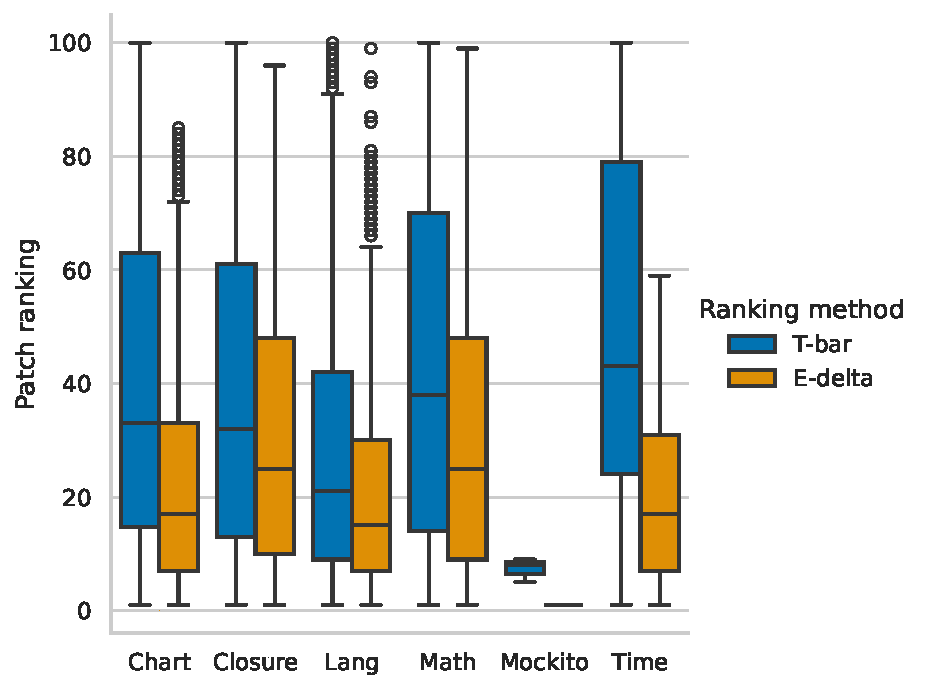
\includegraphics[width=0.8\textwidth]{figures/results/untested_ranking_both.pdf}
  \caption{Entropy-delta and TBar ranking (lower is better) of test-passing
  patches on 72 Defects4J bugs.}
  \label{fig:e-delta-efficiency}
\end{figure}

\begin{figure}[t]
  \centering
  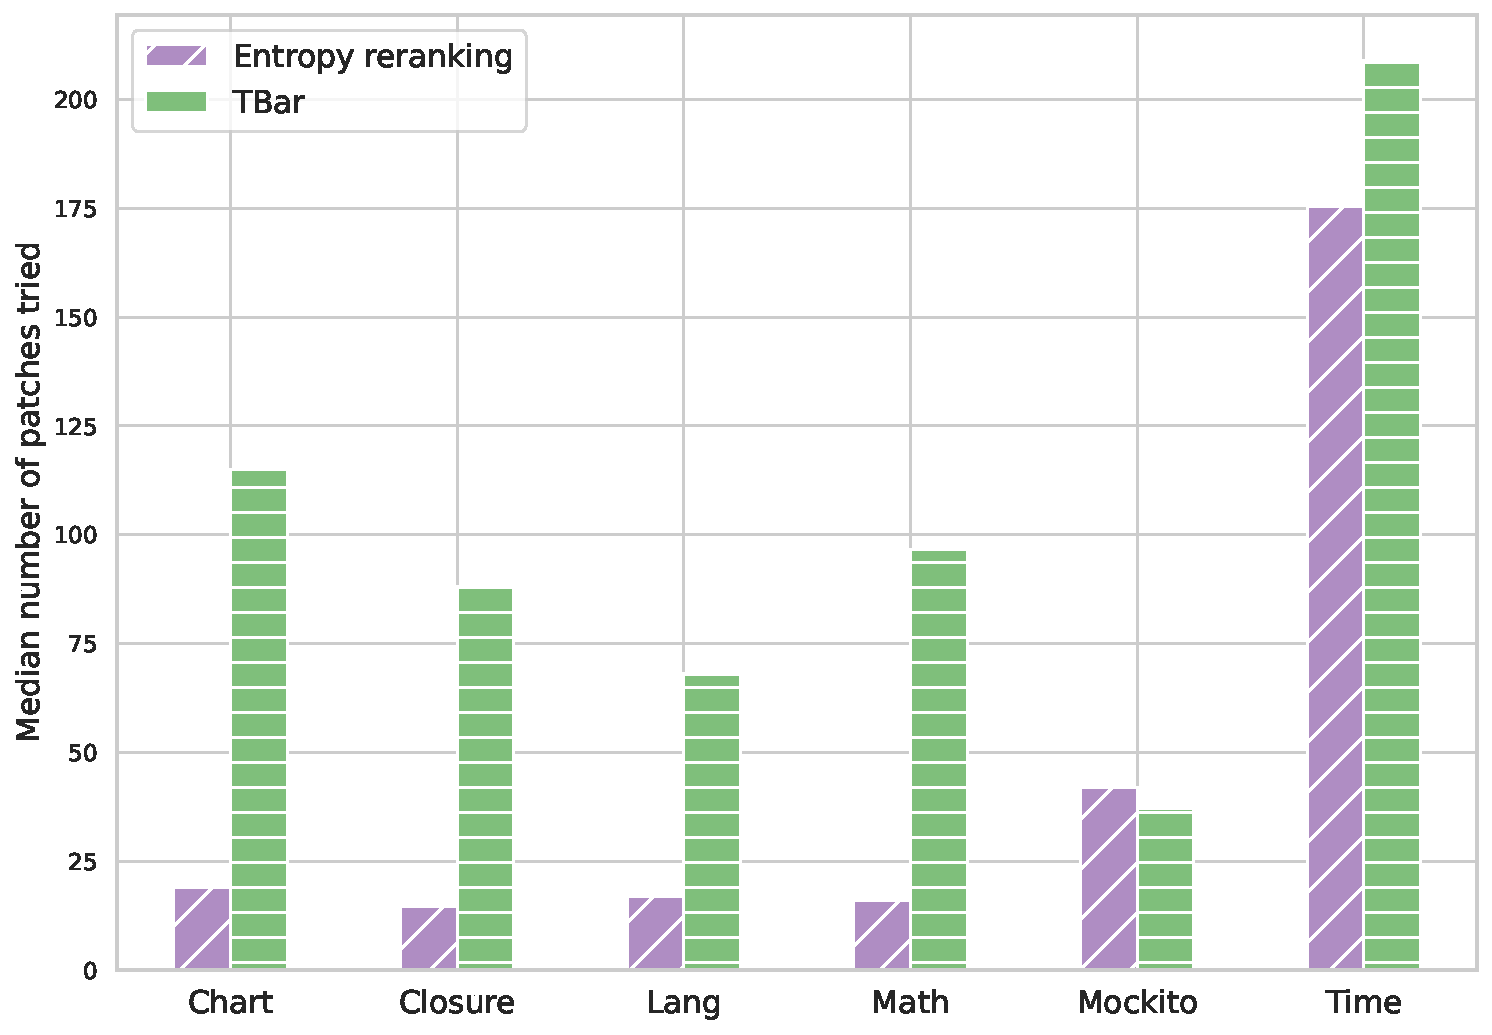
\includegraphics[width=0.8\textwidth]{figures/results/untested_num_patches.pdf}
  \caption{Median number of patches tested (lower is better) per project before successful patch using TBar original ranking and entropy-delta re-ranking of test-passing patches on 100 Defects4J bugs.}
  \label{fig:e-delta-num-patches}
\end{figure}

In this section, we discuss the observed relationship of entropy and
test-passing patches. We use entropy from inCoder. We measure the impact of entropy-delta on patch
generation efficiency with two methods: (1) measuring each successful
(test-passing) patch's ranking as ranked by original TBar and entropy-delta
re-ranked TBar, and (2) incorporating entropy-delta into TBar and measuring the
total number of  patches generated to pass all tests. 

I first configured TBar to generate only 100 patches per each Defects4J bug,
assuming perfect fault localization. Of the TBar patches I generated, 72
passed all tests contained in their bugs' respective repositories (e.g., all
tests written for project Chart). Finally, we calculated the entropy-delta score
for each patch, and the test-passing patch's original ranking according to
TBar. As seen in Table \ref{table:patch_efficiency}, entropy-delta improves 60
out of the 72 rankings as compared to TBar's original ranking. On average, we
observed a mean rank decrease of 24, meaning that using entropy-delta to rank
the generated TBar patches can reduce a mean of 24 full test iterations (i.e.,
each potential patch must run through all test cases in the repository before
knowing if it is a plausible patch). Liu et
al.~\cite{efficiency} compared 16 APR techniques and found that TBar exhibits one of the highest number of patches generated, but also the highest rate of bug fixing across Defects4J.
I posit that entropy-delta's efficiency improvement over TBar significantly boosts template-based APR's overall utility.

Figure~\ref{fig:e-delta-efficiency} compares the TBar ranking
and entropy-delta ranking. Each bar represents the rank of test-passing patches
compared to all generated patches per Defects4J project. A lower rank signifies a
more efficient repair process, as the repair process ends when a test-passing
patch is found. As seen in Figure~\ref{fig:e-delta-efficiency}, TBar's original
ranking for test-passing patches is higher than entropy-delta's ranking across
all projects. Entropy-delta shows a higher disparity on ranking between test
passing and test failing patches (i.e., a lower median rank for all test-passing
patches). In particular, patches from projects Chart and Time show the largest
improvement from re-ranking patches with entropy-delta. Successful patches in
Chart and Time typically require multi-line edits, and with a wider range of
templates to choose from, entropy-delta can make a greater impact in reducing
the number of patches tested.

I then configured TBar to use entropy-delta ranked patches directly, and
measured the total number of patches required until a successful bug fix (i.e.,
passing all tests). Figure~\ref{fig:e-delta-num-patches} shows the median number
of patches tested per project before a successful patch using TBar original
ranking and entropy-delta re-ranking. We observe that entropy-delta re-ranking
reduces the median number of patches tested across all projects except for
Mockito. Mockito has only three single line bugs that TBar can fix. With a smaller total number of patches
to try on a single template (e.g., 11 total possible patches for Mockito-26),
entropy-delta re-ranking does not have as large of an impact on APR efficiency. 


Finally, we measure the actual correctness of TBar's first plausible patch, as ranked by Entropy. 
I find that, of the 72 plausible patches produced by TBar in our experiment, 19 are identical to the developer fix. 

\begin{tcolorbox}
  [colback=white,colframe=black,arc=0pt,boxrule=0.5pt,title=RQ1
 Summary,boxsep=2pt,left=1pt,right=1pt,top=1pt,bottom=1pt,fonttitle=\bfseries]
 I show that entropy can be used to rank patches before going through the
 entire test-suite, thereby reducing the test overhead for template-based repair
 technique TBar by a mean of 24 patches tested. Entropy-delta can both reduce
 the median number of patches tried before finding a fix, and consistently rank
 test patching patches higher than test-failing patches without any dependency
 on the test-suite. Entropy-delta is most useful for bugs that require
 multi-line patches.
\end{tcolorbox}


\noindent\textbf{RQ2. How well does entropy-deltas identify correct patches?}
\begin{table*}[t]
  \centering
\caption{\small Ranking results of 1290 plausible patches per Defects4J project using ranking methods SBFL, Shibboleth, and entropy-delta}
\begin{tabular}{l|lrrrrrr} 
\toprule
 \textbf{Project} & \textbf{\#Patches} & \textbf{\#Correct} &
 \textbf{\#Incorrect} & \textbf{Top-N} & \textbf{SBFL} & \textbf{Shibboleth} &
 \textbf{Entropy-delta}\\
\midrule
\multirow{2}{*}{Chart} & \multirow{2}{*}{201} & \multirow{2}{*}{19} &
\multirow{2}{*}{182} & Top-1              & 3  & 11  & 10   \\
&  &  & & Top-2              & 6  & 14  & 14   \\

\midrule
\multirow{2}{*}{Closure} & \multirow{2}{*}{269} & \multirow{2}{*}{64} &
\multirow{2}{*}{205} & Top-1              & 19  & 27  & 48   \\
&  &  & & Top-2              & 38  & 47  & 58   \\

\midrule
\multirow{2}{*}{Lang} & \multirow{2}{*}{220} & \multirow{2}{*}{35} &
\multirow{2}{*}{185} & Top-1              & 1  & 14  & 20   \\
&  &  & & Top-2              & 12  & 22  & 27   \\

\midrule
\multirow{2}{*}{Math} & \multirow{2}{*}{541} & \multirow{2}{*}{67} &
\multirow{2}{*}{474} & Top-1              & 10  & 27  & 39   \\
&  &  & & Top-2              & 30  & 38  & 55   \\

\midrule
\multirow{2}{*}{Mockito} & \multirow{2}{*}{2} & \multirow{2}{*}{1} &
\multirow{2}{*}{1} & Top-1              & 0  & 1  & 1   \\
&  &  & & Top-2              & 1  & 1  & 1   \\

\midrule
\multirow{2}{*}{Time} & \multirow{2}{*}{57} & \multirow{2}{*}{11} &
\multirow{2}{*}{46} & Top-1              & 3  & 8  & 9   \\
&  &  & & Top-2              & 5  & 5  & 10   \\
\midrule
\multirow{2}{*}{Total} & \multirow{2}{*}{1290} & \multirow{2}{*}{197} &
\multirow{2}{*}{1093} & Top-1              & 36  & 85  & \textbf{127}   \\
&  &  & & Top-2              & 92  & 130  & \textbf{165}   \\
\end{tabular}
\label{table:patch_topn}
\end{table*}


\begin{table}[t]
  \centering
\caption{\small Classification scores of 2,147 plausible patches on Defects4J projects using classification methods PATCH-SIM, Panther, and entropy-delta}
\begin{tabular}{r|rrr}
\toprule
\textbf{Score}  & \textbf{PATCH-SIM}& \textbf{Panther} & \textbf{Entropy-delta}
\\
\midrule
Accuracy  & 0.388 &  0.730 & 0.735\\
Precision  & 0.245 &  0.760 &0.900\\
+ Recall & 0.711 & 0.757 &0.760\\
- Recall & 0.572 &  0.696 &0.624\\
F1  & 0.377 &  0.750 & 0.824\\
\bottomrule
\end{tabular}
\label{table:patch_classification}
\end{table}

\begin{figure}
\centering
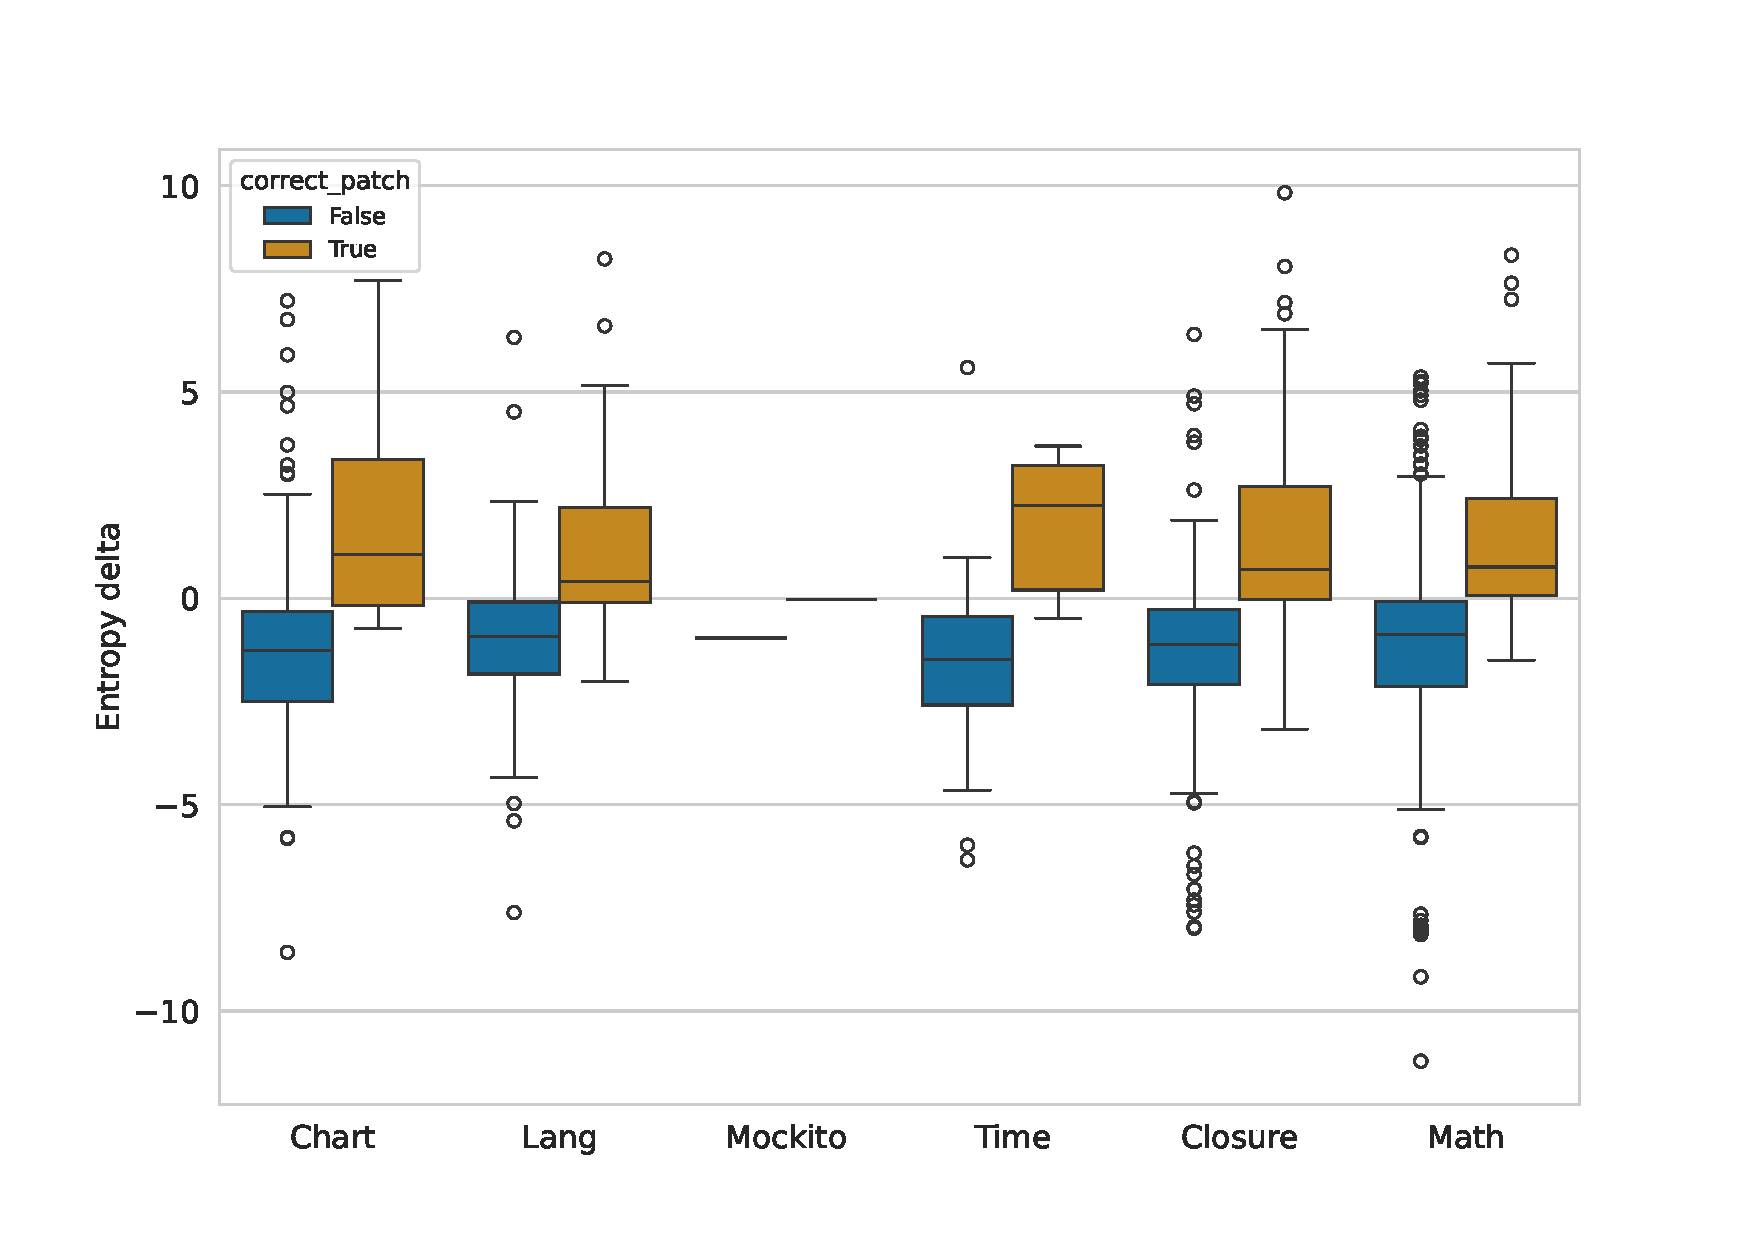
\includegraphics[width=0.7\textwidth]{figures/results/tested_ranking_edelta.pdf}
\caption{Entropy-delta across correct and incorrect patches on Defects4J projects. A
higher entropy-delta signifies a less surprising patch to the LLM, and a lower
entropy (sometimes negative) entropy-delta signifies a more surprising patch to
the LLM.}
\label{fig:e-delta-patch}
\end{figure}

I saw that entropy-delta can improve the efficiency of patch
generation by reducing number of patches tested. However, it is important to
note that a test-passing patch is not necessarily correct. To further explore
the issue of correctness, we investigated the ability of entropy-deltas to
distinguish between correct and incorrect patches, both of which are
test-passing.

\subsubsection{Patch ranking}
I evaluate a dataset of 1,290 patches generated by 7 prior APR methods
collected by Ghanbari et al.~\cite{Shibboleth}. For each bug, the dataset
includes some number of plausible (i.e., test passing) patches, where exactly
one is correct, and the rest are incorrect. We attempt to isolate the true
correct patch from the incorrect patches. We then rank each patch according to
its entropy-delta, querying the model for the entropy of the entire patch region
before and after the replacement. 

Following the approach by Shibboleth~\cite{Shibboleth}, we use Ochiai's SBFL for patch ranking as a baseline: ranking patches by the SBFL suspiciousness of the modified location. 

Table~\ref{table:patch_topn} shows the Top-1
and Top-2 results of our approach on the labeled dataset of 1,290 patches. We
see from Table~\ref{table:patch_topn} that entropy-delta outperforms both SBFL
and Shibboleth~\cite{Shibboleth} on Top-2 across all projects, and entropy-delta outperforms
Shibboleth on Top-1 across all projects but Chart (10 Top-1 as compared to
Shibboleth's 11 Top-1). Overall, we see that entropy-delta improves upon
Shibboleth by 49\% for Top-1, and 27\% for Top-2.

The difference in entropy reduction between correct and plausible but incorrect
patches is shown in greater detail in Figure~\ref{fig:e-delta-patch}. We see a
clear difference in entropy-delta across correct and incorrect patches. In
particular, the correct patches for all six projects have a median entropy-delta
value of above 0, and the incorrect patches for all six projects have a median
entropy-delta value of below 0. A correct patch tends to appear
more natural to the LLM as compared to its original buggy line. 

\subsubsection{Patch classification}

 Table~\ref{table:patch_classification} shows our classification results on a
labeled dataset of 2,147 plausible patches curated by Tian et al.~\cite{Panther}
for classifying patches as correct or incorrect. Entropy-delta 
improves upon the accuracy score of PATCH-SIM~\cite{patch-sim} and Panther~\cite{Panther}, but only slightly
improves +recall score over both PATCH-SIM and Panther. For -recall,
entropy-delta performs better than PATCH-SIM by 9\%, but performs worse than
Panther by 10\%. Entropy-delta slightly improves accuracy over Panther by 0.6\%,
and 89\% over PATCH-SIM. Entropy-delta improves precision over Panther by 18\%,
and PATCH-SIM by 267\%. Finally, entropy-delta performs better than both
PATCH-SIM and Panther on F1 score, by 118\% and 10\% respectively. As compared to the state-of-the-art, entropy improves classification performance on true positives more than true negatives. 


\subsubsection{Patch classification on machine learning APR}
our analysis focused on comparing the degree of entropy reduction between true
correct patches and plausible test-passing patches. As shown in
Table~\ref{table:patch_topn}, Table~\ref{table:patch_classification}, and
Figure~\ref{fig:e-delta-patch}, our results suggest that correct patches
tend to lower entropy (i.e., increase naturalness) more than incorrect patches. 
Specifically, entropy-delta ranks 49\% more correct patches in the Top-1
than the state-of-the-art patch ranker Shibboleth, and entropy-delta can
classify correct patches with an 18\% higher precision than the state-of-the-art
patch classifier Panther. These findings suggest that entropy-deltas can be a
valuable heuristic for distinguishing between correct and incorrect patches.


\begin{tcolorbox}
  [colback=white,colframe=black,arc=0pt,boxrule=0.5pt,title=RQ2
    Summary,boxsep=2pt,left=1pt,right=1pt,top=1pt,bottom=1pt,fonttitle=\bfseries]
    The entropy-delta from a LLM distinguishes between correct and plausible
    (test-passing but incorrect) patches with
    higher precision and accuracy than state-of-the-art patch disambiguation tools.
\end{tcolorbox}


\section{Conclusion}
\label{sec:Entropy-conclusion}
After fault localization, a natural next step of software maintenance is program repair. 
In this chapter, we introduce the use of ``unnaturalness'' of code for automated
program repair through the measurement of entropy generated by code-tuned LLMs.
I coin the term entropy-delta, which measures the difference in
entropy between a proposed code insert (i.e., a patch) and the original code. We use entropy-delta on untested patches to save an average of 24
test runs per bug for the template-based APR technique \textit{TBar}. Entropy-delta can improve upon state-of-the-art patch ranking by 49\% for Top-1,
can classify plausible patches with a 18\% higher precision, and is still effective  for patches produced by modern ML-based tools. The results in this chapter
indicate that LLMs can be a powerful addition to state-of-the-art APR tools
without the dependency on tests, and the usage of LLM code generation. The
reduction in both test suites and LLM code generation results in the reduction
in model over-fitting and training data leakage.








\chapter{Program Transpilation}
\label{ch:vert}
A common component of software evolution is program translation, whether between platforms, software versions, or programming languages. Specifically, translating from one programming to another while directly compiling the target program is called program transpilation.
One key difficulty in program transpilation is producing idiomatic code.
In this chapter, we design, implement, and evaluate a LLM-based transpilation tool, and show that it is more idiomatic than prior non-LLM transpilers. Specifically, we use the Rust programming language as a case-study for our target transpiling language.

Rust is a programming language that combines memory safety and
low-level control, providing C-like performance while guaranteeing the absence of undefined behaviors by default. Rust's growing popularity has prompted research on safe and correct transpiling of existing code-bases to Rust. Existing work falls into two categories: rule-based and large
language model (LLM)-based. While rule-based approaches can
theoretically produce \textit{correct} transpilations that maintain input-output equivalence to the original, they often yield
unidiomatic Rust code that uses unsafe subsets of
the Rust language. On the other hand, while LLM-based approaches typically produce more idiomatic, maintainable, and safe code, they do not provide any guarantees about correctness.

In this work, we propose VERT (verified equivalent Rust transpilation with LLMs), a tool that can produce idiomatic Rust transpilations with formal guarantees of correctness. VERT's only requirement is that there is Web
Assembly compiler for the source language, which is true for most major languages. 

\section{VERT: Verified Equivalent Rust Transpilation with LLMs}
\label{section:methodology}

\begin{figure}
\centering
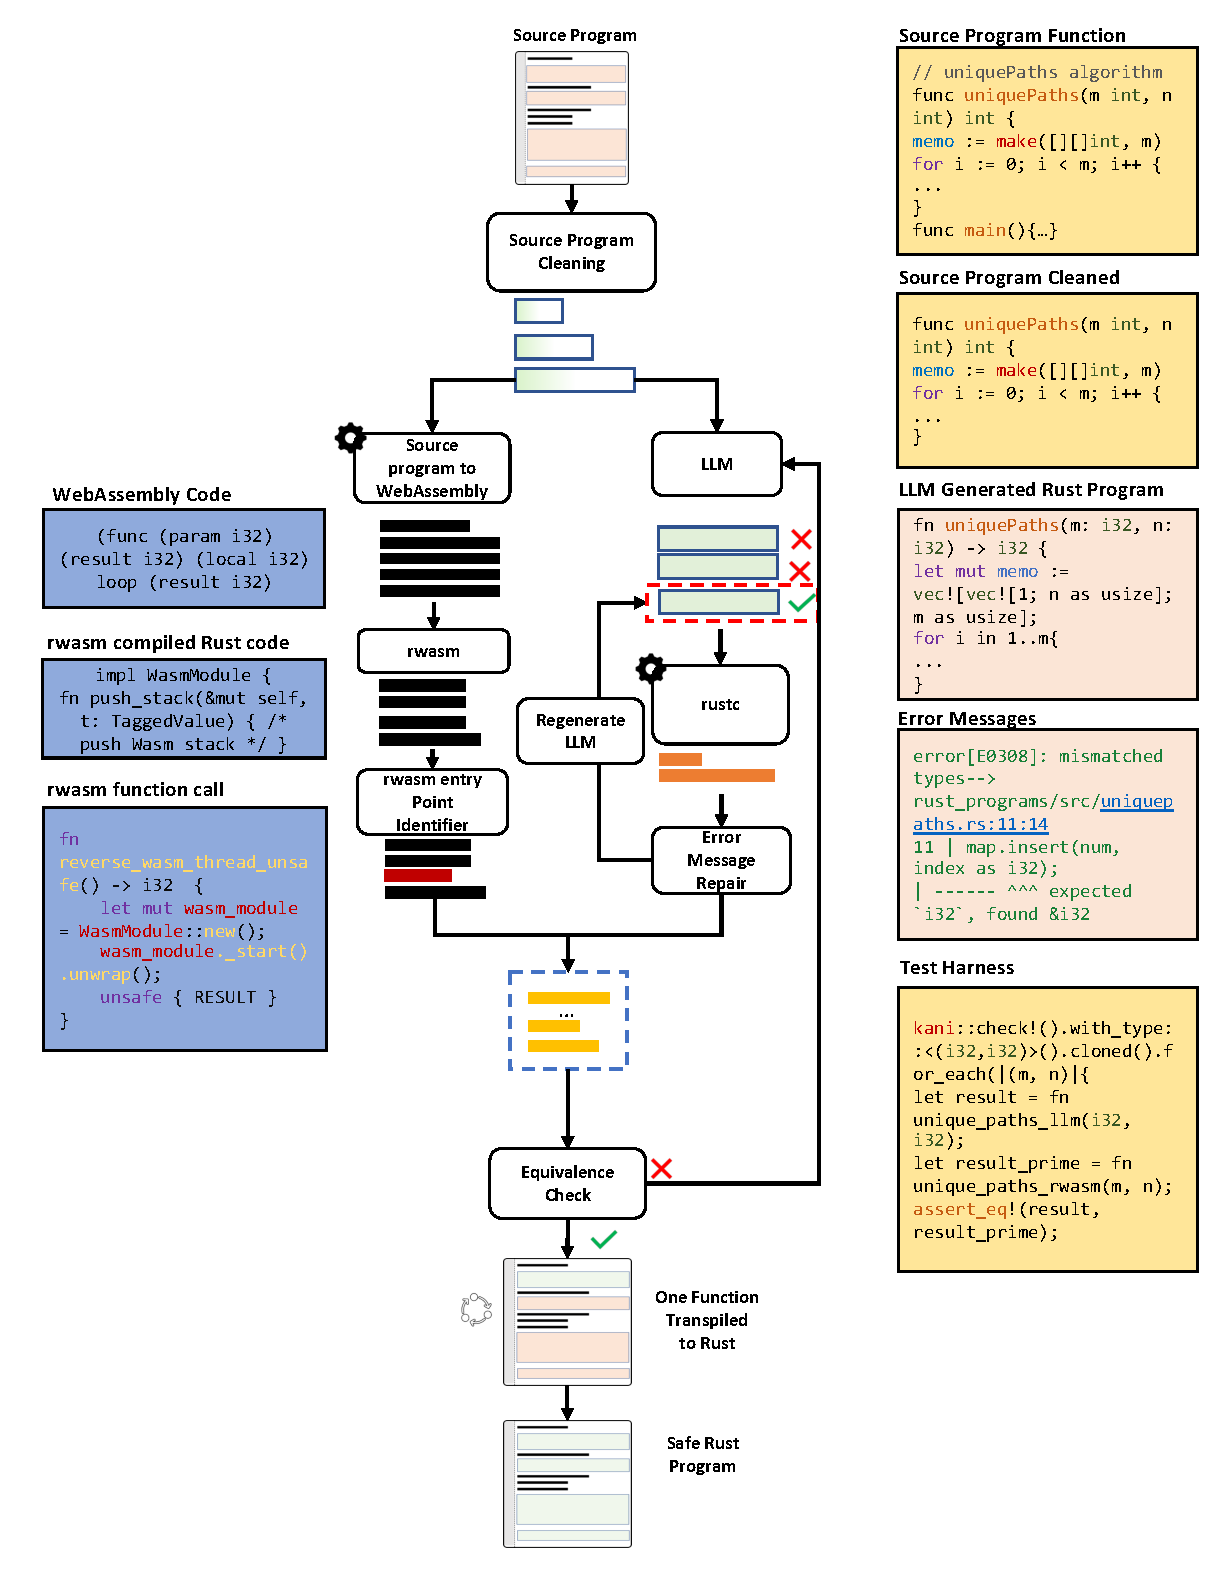
\includegraphics[width=0.95\textwidth]{figures/approach/gotorust_approach.pdf}
\vspace*{-3mm}
\caption{\small VERT’s architecture, which takes as input a source program and produces a formally equivalent Rust program}
\label{fig:overview}
\end{figure}

In this section, we describe the key ideas behind VERT, a universal Rust transpilation technique.
Figure~\ref{fig:overview} gives an overview of VERT's entire pipeline. The technique takes as input a source program, and outputs a verified equivalent Rust program. As shown in Figure \ref{fig:overview}, we parse the program into separate functions during the cleaning phase, then split the pipeline into two paths. The first path outputs a LLM-generated Rust transpilation. The second path produces rWasm Rust code that is compiled directly from the original program through Wasm. Finally, we create a test harness based on the original program to verify equivalence of the two paths' outputs, and only after a successful verification I output a correct and maintainable Rust transpilation. In the following sections, we describe each component of VERT in further detail.


\subsection{Program repair on LLM output}
\label{sec:repair}
LLMs often produce incorrect code. When prompting a LLM for Rust code, any slight mistake could cause the strict Rust compiler (\lstinline{rustc}) to fail. Fortunately, \lstinline{rustc} produces detailed error messages when compilation fails to guide the user to fix their program. We create an automatic repair system based on \lstinline{rustc} error messages. For each error, we first classify the error into one of three main categories: syntax, typing, and domain specific. 


As seen in Figure \ref{code:error1}, an example syntax error generated by the LLM is the wrong closing delimiter. For \lstinline{rustc} to successfully compile, all syntax errors must be resolved. We track the error code location (e.g., line 10 in Figure \ref{code:error1}), and I use the \lstinline{rustc} provided initial delimiter to guide our repair strategy. For this case, we know to use the right curly bracket \lstinline{\} to replace \lstinline{]} on line 10. 

Typing error messages in Rust generally have a similar structure. In particular, error messages are usually of the form \lstinline{expected type a, found b}. Figure~\ref{code:error2} shows the LLM generate a pass-by-reference variable \lstinline{&i32} while \lstinline{rustc} expects a pass-by-value \lstinline{i32}. Using the compiler message's error localization and suggestion line (characterized by the keyword \lstinline{help}), we replace the variable \lstinline{num} by \lstinline{&num}. 

Finally, domain-specific errors are compilation errors that are specific to the program. The error messages for domain-specific errors do not share the same structure, and therefore I only use the \lstinline{rustc} error message suggestion line to generate a repair. In Figure~\ref{code:error3}, which shows the error message for an immutable assignment, the suggestion line indicates that if the variable \lstinline{x} is converted to a mutable object, the immutable assignment error would be solved. Using this suggestion line, we replace \lstinline{x} by \lstinline{mut x}, and observe that the program compiles. It is often the case that even with the error message suggestion line, we cannot generate a repair that fixes all errors. In these cases, we regenerate a LLM output using the error as part of the new prompt and restart the process. Our error-guided repair is significantly faster than the LLM generation (discussed in Section~\ref{section:results}), so I only regenerate a LLM output after exhausting all \lstinline{rustc} helper messages.


\begin{figure}[t]
\centering
    \begin{lstlisting}[numbersep=5pt,xleftmargin=21pt,numberstyle=\scriptsize,basicstyle=\footnotesize\ttfamily,firstnumber=1, language=C]
error: mismatched closing delimiter: ']'
1  | fn roman_to_int(s: &str) -> i32 {
   |                                 ^ unclosed delimiter
10 |     ]);
   |     ^ mismatched closing delimiter
\end{lstlisting}
\vspace*{-2mm}
\caption{\small Syntax error}
\label{code:error1}
\end{figure}

\begin{figure}[t]
\centering
\begin{lstlisting}[numbersep=5pt,xleftmargin=21pt,numberstyle=\scriptsize,basicstyle=\footnotesize\ttfamily,firstnumber=1, language=C, language=C]
error[E0308]: mismatched types-->
11 | map.insert(num,index as i32);| -- ^^^ expected '&i32', found i32
help: consider borrowing here: '&num'
\end{lstlisting}
\vspace*{-2mm}
\caption{\small Mismatched type error}
\label{code:error2}
\end{figure}

\begin{figure}[t]
\centering
\begin{lstlisting}[numbersep=5pt,xleftmargin=21pt,numberstyle=\scriptsize,basicstyle=\footnotesize\ttfamily,firstnumber=1, language=C]
error[E0384]: cannot assign to immutable argument 'x'
1  | fn reverse(x: i32) -> i32 {
   |- help: consider making this binding mutable: 'mut x'
...
16 |         x = x / 10;
   |         ^^^^^^^^^^ cannot assign to immutable argument
\end{lstlisting}
\vspace*{-2mm}
\caption{\small Immutable assignment error}
\label{code:error3}
\end{figure}


% \begin{wrapfigure}{l}{0.5\textwidth}
\begin{figure}
\centering
% \begin{minted}[
% frame=lines,
% framesep=2mm,
% baselinestretch=1.2,
% fontsize=\footnotesize,
% linenos
% ]{Go}
\begin{lstlisting}[numbersep=5pt,xleftmargin=21pt,numberstyle=\scriptsize,basicstyle=\footnotesize\ttfamily,firstnumber=1, language=C]
func callReverse() int {
  result := reverse(123)
  if result == 321 {return 0} 
  else {return 1}
}
\end{lstlisting}
\vspace*{-2mm}
\caption{\small An entry point for the {\tt reverse} function}
\label{code:gotestreverse}
\end{figure}
% \end{wrapfigure}

\subsection{Transpilation Oracle Generation}
Since the LLM output cannot be trusted on its own, we create an
alternate trusted transpilation pipeline for generating a reference Rust
program against which the LLM output is checked. The alternate
pipeline does not need to produce maintainable code, but it needs to translate the source language into Rust using a reliably correct rule-based
method. We use Wasm as the intermediate representation because
many languages have compilers to Wasm, allowing it to serve as the
common representation in the rule-based translation. Once the
input programs are compiled to Wasm, we use
rWasm~\cite{bosamiya2022provably}, a tool that translates from Wasm to
Rust by embedding the Wasm semantics in Rust source code. While the
original authors intended rWasm as a sandboxing tool that leverages
the memory safety properties of safe Rust, we use it to generate
trusted Rust code with same semantics as the original input.

\subsection{Mutation Guided Entry Point Identification}
Given the assembly-like output of rWasm, we must perform analysis to
identify the entry point of the rWasm transpiled function. VERT
provides the option for the user to manually identify the entrypoint,
but I can find it automatically using a simple heuristic, such as a function call or a single test case. We note that this heuristic could be generated automatically using LLMs or search-based software testing and thus I can assume an entrypoint generator in the source language. VERT uses a function call in the source language with constant
inputs to the function to be transpiled and an assertion on the output
of that function. One such function is given in Fig.~\ref{code:gotestreverse}.

% \begin{wrapfigure}{l}{0.5\textwidth}
\begin{figure}
\centering
% \begin{minted}[
% frame=lines,
% framesep=2mm,
% baselinestretch=1.2,
% fontsize=\footnotesize,
% linenos,
% highlightlines={6,9}
% ]{Rust}
\begin{lstlisting}[numbersep=5pt,xleftmargin=21pt,numberstyle=\scriptsize,basicstyle=\footnotesize\ttfamily,firstnumber=1, language=C]
fn func_4(&mut self, ) -> Option<i32> {
  let mut local_3 : i32 = 0i32;
  let mut local_4 : i32 = 0i32;
  v0 = TaggedVal::from(321i32);
  // mutant: v0 = TaggedVal::from(654i32);
  local_3 = v0.try_as_i32()?;
  v0 = TaggedVal::from(123i32);
  // mutant: v0 = TaggedVal::from(456i32);
  local_4 = v0.try_as_i32()?;
}
\end{lstlisting}
\vspace*{-2mm}
\caption{\small The difference between the original rWasm output and the
  mutated one (highlighted).}
\label{code:gotestwasm}
\end{figure}
% \end{wrapfigure}

I leverage this function call to identify the input and output of the
function. While one option for such analysis is to perform
decompilation, we find that a mutation-guided approach is sufficient
for our purposes. In Fig.~\ref{code:gotestreverse}, we know that the
input is \lstinline{123} and the output is \lstinline{321}. Now, we wish to
identify the equivalent constant in the rWasm output. While it is
possible to just perform a linear scan of the rWasm output for this
constant, that risks spurious matches, especially for simple types
like \lstinline{i32}. Instead, we guide this identification by leveraging
the function call and mutating it. Suppose I swap \lstinline{123} with
\lstinline{456} and \lstinline{321} with \lstinline{654} and re-transpile with
rWasm. These constants will change, but the rest of the rWasm output
remains the same. Taking the diff, we can identify inputs and outputs
by what changed. The diff in the rWasm output is shown in
Fig.~\ref{code:gotestwasm}.

\subsection{Equivalence Harness Generation}
In our final step, we generate harnesses to check for equivalence
given the input and output locations. We define equivalence here in
functional terms: for all inputs, running both functions yields no
crashes and identical outputs. To check this property holds, we automatically
generate a wrapper to the Wasm function and a harness where the
LLM-synthesized and wrapped rWasm functions are called with the same
inputs, and the outputs are asserted to be equal. To ensure this
equivalence holds for all inputs, we leverage property-based testing
with random inputs and model-checking with symbolic inputs. For the
remainder of this section, we refer to both of them together as ``the
input.''

The wrapper consists of two parts: input injection, and output
checking. We replace constants inputs with the inputs of the harness
like \lstinline{input: i32}. Instead of replacing the parameters to the
function, we use globals in Rust to inject the inputs right at the
location where constants used to be. An example is given in
Fig.~\ref{code:eqharness}, with \lstinline{func_4} being the Wasm
equivalent of the test. Note that, while this injection requires
unsafe code, it is fine as this is only done in the oracle and the
oracle is discarded once the equivalence is checked.
%
I inject the baseline \lstinline{OUTPUT_1} and assert that the function
returns $0$. Since the function returns $0$ when output equals the
injected value, we know the functions returned the same value.

I note that while this approach is sound, it may falsely identify
some equivalent programs as faulty due to semantic differences between
Rust and the target language, or between the target language and
rWasm{} embedding. We note two cases where I permit the analyst to
add assumptions. First, when the input type is an unsigned integer,
the analyst may assume nonzero values even though compilers may
represent it as signed. Second, the analyst may restrict the range of
strings to ASCII when the input is a C program to avoid crashing the
Wasm with Rust's Unicode strings.

\begin{figure}
\centering
% \begin{minted}[
% frame=lines,
% framesep=2mm,
% baselinestretch=1.2,
% fontsize=\footnotesize,
% linenos
% ]{Rust}
\begin{lstlisting}[numbersep=5pt,xleftmargin=21pt,numberstyle=\scriptsize,basicstyle=\footnotesize\ttfamily,firstnumber=1, language=C]
static mut INPUT_1 = 0;
static mut OUTPUT_1 = 0;
impl WasmModule {
  /// returns 0 if the output matches
  fn func_4(&mut self, ) -> Option<i32> {
    // ...
    let mut local_3 : i32 = 0i32;
    let mut local_4 : i32 = 0i32;
    v0 = TaggedVal::from(unsafe {INPUT_1});
    local_3 = v0.try_as_i32()?;
    v0 = TaggedVal::from(unsafe {OUTPUT_1});
    local_4 = v0.try_as_i32()?;
    // ...
  }
}
/// equivalence-checking harness.
fn equvalence() {
  bolero::check!()
  .for_each(|(input: i32)| {
    let llm_fn_output = llm_generated_reverse();
    unsafe {
      INPUT_1 = input;
      OUTPUT_1 =  llm_fn_output;
    }
    let mut wasm_module = WasmModule::new();
    wasm_module._start().unwrap();
    assert!(wasm_module.func_4().unwrap() == 0);
  });
}
\end{lstlisting}
\caption{\small Equivalence-checking harness for {\tt func\_4}.}
\label{code:eqharness}
\vspace*{-5mm}
\end{figure}
% \end{wrapfigure}

\subsection{Equivalence Checking}

With the equivalence checking harness built, we must now drive the harness and check that the equivalence property holds for all inputs. VERT provides two equivalence checking techniques with increasing levels of confidence and compute cost.
I use existing tools that operate on Rust to
prove equivalence between the LLM-generated and the rWasm-generated oracle Rust programs. We use Bolero, a Rust testing and verification framework that can check properties using both Property-Based Testing (PBT)~\cite{fink1997property} and Bounded Model Checking (BMC)~\cite{clarke2001bounded,DBLP:conf/tacas/ClarkeKL04}.

\subsubsection{PBT}
PBT works by randomly generating inputs to the function under
test, running the harness with these inputs, and asserting the desired
properties (e.g., equivalence between two functions). PBT repeatedly runs this procedure to
check the property over the range of inputs. PBT is a valuable tool for catching implementation bugs,
however it is generally infeasible to run PBT for long enough to exhaust all possible inputs to a program.

First, we run the equivalence-checking
harness with PBT using Bolero up to the time limit, generating random
inputs and checking equivalence of the outputs. If the candidate
diverges from the oracle, then PBT will return the diverging input as
a counterexample. If no counterexample is found within the time limit,
I say this candidate passes PBT.

\subsubsection{BMC}
If the PBT stage succeeds, we now perform bounded verification with
a combination of Bolero and Kani. 
I customize Bolero to perform model checking through Kani~\cite{vanhattum2022kani},
a model-checker for Rust. When run with Kani, Bolero produces
symbolic inputs rather than random concrete inputs. Executing the
harness with symbolic inputs, we can cover the entire space of inputs
in one run and the model-checker ensures the property holds for all
possible inputs. Since symbolic execution does not know how many times
loops are run, Kani symbolically executes loops up to an user-provided
bound. To prove soundness of this bound, Kani uses {\it unwind checks}
asserting that loop iteration beyond the bound is not reachable. 

I run Kani with an unwinding bound of $k$ (where $k = 10$) and \textit{no unwind checks}. This means that paths up
to $k$ loop iterations is exhaustively explored, but any divergences
between the candidate and the oracle with traces containing more than
$k$ loop iterations are missed. We run this phase for 120 seconds, and
terminate with 3 potential results. First, Kani returns with a
counterexample that causes the oracle and the candidate to diverge or
one of the two to crash. Second, Kani does not return with an answer
within the time limit, which I also consider to be a failure as we
cannot establish bounded equivalence. Finally, Kani verifies that,
limited to executions with at most $k$ loop iteration, there are no
divergences or crashes. We consider the third case alone to be
successful. 

Although for finite-input, deterministic programs, it is possible to
perform verification with full exhaustive unwinding using Kani (i.e.,
fully verifying all $k$ until exhaustion), we measure that the median
time to exhaustively verify a Rust program within our selected dataset
is 5 minutes, which is much longer than our established time limit of
120 seconds per program. We choose not to use full Kani verification
as a metric due to time and compute constraints.


I support complex types through their primitive parts. Given a struct
or enum, that Kani or Bolero does not initially support, we construct
values of that type by abstracting the primitive parameters of that
type and any required discriminants for enums. For types of finite
size, this is sufficient. However, we provide bounded support for
handling vector types. The challenge here is to vary the length of the
vector in the rWasm output, which is done by having a fixed-length
vector of varying inputs and then pruning the length down to the
actual length dynamically. Our approach is sound and complete for
primitive types, and by extension, any type that comprises solely of
primitive types such as tuples of primitives. For unbounded types like
vectors, hashmaps and user-defined types containing such, VERT
synthesizes harnesses that generate inputs up to the size encountered
in the sample function call. As a limitation, any divergences that
require larger vector than encountered will be missed.


\subsection{Few-shot Learning}
\label{sec:fewshot}
The main focus of this work is on verifying the output of LLMs for program transpilation, and not LLM prompt engineering. Therefore, we keep the prompts simple and short. Complicated and repeated querying of the same prompts do not provide additional benefits on the accuracy of outputs for small sized models, and too expensive for an average practitioner for industry sized models (i.e., Anthropic Claude).
To achieve few-shot learning on our transpilation queries, each failed transpilation attempt provides its equivalence checking counter examples as a few-shot learning example for future transpilation attempts. 

Figure.~\ref{code:prompt} shows our template for few shot learning. We start with querying the LLM to refactor the source code into safe Rust. Although I filter for safe Rust LLM output, we experimentally found that asking the LLM to always produce safe Rust gives more accurate results. We prompt the LLM to use the same argument and return types as the original, and can compile without external dependencies. Finally, we collect the counter examples from prior failed equivalence checks as part of the prompt. Specifically, we ask the LLM to consider the specific inputs that caused a test or verification failure from the previous iterations. We observed that providing specific inputs as information to the LLM results in subtle bug fixes within the program output.

\begin{figure}
\centering
\begin{lstlisting}[numbersep=5pt,xleftmargin=21pt,numberstyle=\scriptsize,basicstyle=\footnotesize\ttfamily,firstnumber=1, language=C]
{Original code}
Safe Rust refactoring of above code in {language}.
Use the same function name, same argument and return types.
Make sure the output program can compile as a stand alone.
// If there exists counter examples from prior failed 
// equivalence checking Test that outputs from inputs {counter_examples} 
// are equivalent to source program.
\end{lstlisting}
\caption{\small LLM Prompt template.}
\label{code:prompt}
\vspace*{-5mm}
\end{figure}
%%% Local Variables:
%%% mode: latex
%%% TeX-master: "../main"
%%% End:


\section{Evaluation Setup}
\label{section:eval}

In this section, we present our evaluation setup for the following research questions.

\noindent\textbf{RQ1. How does VERT perform vs. using the respective LLM by itself?}
I evaluate our technique's performance on a benchmark dataset,
showing that VERT significantly increases the number of verified equivalent transpilations vs. using the LLM by itself.

\noindent\textbf{RQ2. How does each component of VERT's approach impact its performance?}
I conduct an ablation analysis, which shows that our prompting and
error-guided refinement helps produce more well-typed and more correct
programs.
I further measure the runtime performance of each part of VERT, showing that
time costs of error-guided refinement is reasonable and VERT
spends most of the time in verification. 

\subsection{LLM Fine-tuning}
The availability of Rust code in open source is scarce as compared code written in most other programming languages. Incoder~\cite{fried2022incoder} estimates that Rust is only the 20th most common language in their training database, which is a 159GB code corpus taken from Github BigQuery \footnote{https://cloud.google.com/blog/topics/public-datasets/github-on-bigquery-analyze-all-the-open-source-code}. Due to the lack of Rust data available on open-source, we opt to not train a LLM targeted at Rust code generation. Instead, we directly use an off-the-shelf industry grade LLM, and also fine-tune on a separate open-source pretrained LLM. Specifically, we use Anthropic Claude-2 \footnote{https://www.anthropic.com/product} for the industry grade LLM, and StarCoder~\cite{li2023starcoder} for the pretrained LLM. 

I use light weight and parameter efficient adapter layers~\cite{hu2023llm, yang2024large, peft} for fine-tuning StarCoder. 
% Instead of retraining StarCoder entirely, we taken the final hidden states of StarCoder and add adapter layers at the end using small amounts of data.
I collect 94 LeetCode type question solutions in C, C++, Go and Rust. Although there are existing code bases for all four languages, we find that LeetCode has the most consistent translation between other languages and Rust. We were able to collect 94 LeetCode questions of which have a direct translation between all 3 languages.

For each LeetCode type question, we have a corresponding source program (written in Go, C, or C++), and a target program (written in Rust). We encode all code words into tokens using the GPT-2 tokenizer. We fine-tune with 4 Transformer layers, 300 total epochs, and a final model dimension of 6144.

\subsection{Benchmark selection}
I draw our benchmarks from two sources. Our first source is the benchmark set from TransCoder-IR \cite{szafraniec2022code}, which is primarily made up of competitive program solutions. In total, this benchmark set contains 852 C++ programs, 698 C programs, and 343 Go programs. We choose this dataset to avoid potential data-leakage (i.e., LLM memorization)~\cite{biderman2024emergent} in our evaluation. We note that the Rust programs produced by TransCoder-IR were released after June 2022, which is the training data cutoff date of our chosen LLMs~\cite{li2023starcoder, claude, codellama}. 
I select programs from the TransCoder-IR dataset that can directly compile to Wasm using rWasm. After filtering, we collect a benchmark set of 569 C++ programs, 506 C programs, and 341 Go programs. 
These types of benchmarks are common for evaluating LLMs' coding ability. However, the programs themselves often do not make extensive use of pointers, so they do not adequately challenge VERT{}'s ability to generate safe Rust. 


To provide insight into~VERT{}'s ability to write safe rust, we gather 14 additional pointer-manipulating C programs from prior work on C to Rust transpilation~\cite{C2Rust, zhang2023ownership, emre2021translating}. We note, however, that the benchmarks in these prior works use open-source programs written before our chosen LLM's training data cutoff (June 2022). To avoid LLM data-leakage, we select and customize snippets from these C projects to transpile to Rust. We manually label the input output pairs for each snippet for verifying equivalence on the transpiled Rust programs. Many of the benchmarks I select involve multiple functions. The explicit goal when selecting benchmarks from these projects is to discover the limitations of~VERT{} in terms of writing safe Rust, therefore I gather benchmarks of increasing complexity in terms of the number of pointer variables, and the number of functions in the benchmark. We present several complexity metrics for the benchmarks and discuss them in more detail in Section~\ref{section:results}. 

In total, we evaluate our approach on \textbf{569 C++} programs, \textbf{520 C} programs, and \textbf{341 Go} programs.


\subsection{Evaluation Metrics}
Neural machine translation (NMT) approaches use
metrics that measure token similarity between the expected output and the actual output produced by the LLM. While these approaches are often meaningful when applied to natural language, for programming languages, small differences in the expected output and actual output could result in different compilation or run-time behavior.
Conversely, two programs that share very few tokens (and hence have a very low text similarity score) could have identical compilation or run-time behavior.
For programming languages, metrics based off of passing tests have been proposed. Roziere et al.~\cite{roziere2020unsupervised} and Szafraniec
et al.~\cite{szafraniec2022code} use the computational accuracy (CA)
metric, which counts a translation as correct if it passes a series of
unit tests. However, there is no accepted standard for the
number of required passing tests when using the CA metric. Furthermore, the CA metric does not take into
account the quality or coverage of the unit tests.

To improve upon the metrics used for prior NMT approaches and remove the overhead of writing high-coverage unit tests, we use formal methods to measure the correctness of the output. In particular, we use property based testing (PBT) and bounded model checking (BMC). We insert the LLM-generated code and rWasm-generated code in an equivalence-checking harness that asserts equal inputs lead to equal outputs. An example of such a harness is given in Figure~\ref{code:eqharness}. 
% our full procedure is shown in Fig.~\ref{fig:eval}. 
Since the two metrics used are significantly
slower than checking a series of unit tests, we set a time limit for
our metrics. For both metrics, we set a 120 seconds limit. For
PBT, no counterexamples within 120 seconds counts as success. For BMC, success requires establishing verified equivalence within 120 seconds. If either of the step fails, VERT terminates.


\section{Results}
I present results on the TransCoder-IR benchmarks in Table~\ref{table:results}. We present VERT{} operating in three different modes. \textit{Single-shot} means that VERT{} uses the LLM \textit{once} to create a single candidate transpilation, and then proceeds directly to verification. If verification fails, then VERT{} does not attempt to regenerate. 
\textit{few-shot} means that, if verification fails, then VERT{} will prompt the LLM to regenerate the transpilation repeatedly. In each iteration, we apply the syntactic repair described in Section~\ref{sec:repair} to the output of the LLM. Finally, \textit{few-shot counter examples} means that I use counter examples produced by previous failed verification attempts as part of the LLM's few-shot learning, as described in Section~\ref{sec:fewshot}. \textit{few-shot counter examples} only works for instruction-tuned models. We re-prompt the LLM up to 20 times for few-shot modes. For each LLM and each mode of VERT{}, we report the number of transpilations that compiled and that passed the various verification modes. As seen in Table~\ref{table:results}, we only perform \textit{single-shot} for Transcoder-IR (baseline) to replicate results from prior work. We perform \textit{few-shot} on CodeLlama2 and StarCoder fine-tuned to investigate the effectiveness of few-shot and rule-based repair on open-source, non-instruction tuned LLMs. Finally, we perform \textit{single-shot, few-shot, and few-shot with counter examples} with Anthropic Claude-2 to investigate how each part of VERT impacts an instruction-tuned LLM's ability to perform Rust transpilation.

\label{section:results}

\noindent\textbf{RQ1. How does VERT perform vs. using the respective LLM by itself?}



\begin{table}[t!]
\caption{\small VERT performance across with different LLMs and modes.}
\begin{tabular}{l|lp{3cm}rrr}
\toprule
 \textbf{LLM} &  \textbf{Source Lang} & \textbf{Technique} & \textbf{Compiled} & \textbf{PBT} & \textbf{BMC} \\
\midrule

\multirow{3}{*}{TranscoderIR(Baseline)}
& C++ (569)
& Single-shot             & 107  & 23 & 3  \\
\cmidrule{2-6}
& C (520)
& Single-shot             & 101  & 14 & 1  \\
\cmidrule{2-6}
& Go (341)
& Single-shot             & 24  & 3 & 0  \\
\midrule

\multirow{3}{*}{CodeLlama2 13B}
& C++ (569)
& Few-shot    & 307  & 25 & 6  \\
\cmidrule{2-6}
& C (520)
& Few-shot    & 160 & 18 & 4  \\
\cmidrule{2-6}
& Go (341)
& Few-shot     & 104 & 15 & 2 \\
\midrule

\multirow{3}{*}{StarCoder fine-tuned 15.5B}
& C++ (569)
& Few-shot              & 253  & 79 & 8  \\
\cmidrule{2-6}
& C (520)
& Few-shot     & 179 & 76 & 4  \\
\cmidrule{2-6}
& Go (341)
& Few-shot     & 134 & 59 & 2  \\
\midrule
\multirow{9}{*}{Claude-2 130B}
& \multirow{4}{*}{C++ (569)}
& Single-shot            & 240  & 55 & 6  \\
& & Few-shot     & 539 & 292 & 41  \\
& & Few-shot  counter examples  (VERT) & \textbf{539} & \textbf{295} & \textbf{233} \\
\cmidrule{2-6}

& \multirow{4}{*}{C (520)}
& Single-shot            & 239  & 49 & 6  \\
& & Few-shot     & 339 & 195 & 29  \\
& & Few-shot  counter examples (VERT) & \textbf{339} & \textbf{209} & \textbf{193}  \\
\cmidrule{2-6}

& \multirow{4}{*}{Go (341)}
& Single-shot             & 126  & 26 & 3  \\
& & Few-shot      & 276 & 157 & 39  \\
& & Few-shot  counter examples (VERT) & \textbf{317} & \textbf{195} & \textbf{159}  \\
\bottomrule
\end{tabular}
\label{table:results}
\end{table}



\begin{table}[t!]
\centering
\caption{\small VERT's average runtime per component for a Single-program translation}
\begin{tabular}{llr}
\toprule
\textbf{Component type} & \textbf{Component} & \textbf{Time (s)}\\
\midrule\multirow{3}{*}{LLM}
& Transcoder-IR & 8 \\
& CodeLlama-2 & 43 \\
& Starcoder fine-tuned & 45 \\
& Anthropic Claude & 30 \\

\midrule\multirow{3}{*}{Rust compilation}
& $\texttt{rustc}$ & $<1$ \\
& Error guided  & 1 \\
& $\texttt{rwasm}$ & $<1$ \\

\midrule\multirow{3}{*}{Testing and verification}
& PBT & 25 \\
& Bounded-ver. & 52 \\

\bottomrule
\end{tabular}
\label{table:time}
\end{table}

As seen in table~\ref{table:results}, VERT with Claude-2 compiles for 76\% more programs for C++, 75\% for C, and 82\% for Go as compared to baseline (i.e., Transcoder-IR).
VERT with Claude-2 can pass PBT for 49\% more programs for C++, 37\% for C, and 56\% for Go as compared to baseline.
VERT with Claude-2 can pass BMC for 40\% more programs for C++, 37\% for C, and 47\% for Go as compared to baseline.

VERT with both CodeLlama2 and StarCoder fine-tuned also improve upon baseline on number of programs passing compilation, PBT, and BMC. We observe that few-shot learning with rule-based repair on general code-based LLMs can perform more accurate Rust transpilations than a LLM trained with transpilation as its main target.

\begin{tcolorbox}
[colback=white,colframe=black,arc=0pt,boxrule=0.5pt,title=RQ1 Summary,boxsep=2pt,left=1pt,right=1pt,top=1pt,bottom=1pt,fonttitle=\bfseries]
VERT with CodeLlama2, StarCoder fine-tuned, and Anthropic Claude-2 can produce more compiling, PBT, and BMC passing Rust transpilations than baseline. In particular, VERT with Claude-2 can pass BMC for 40\% more programs for C++, 37\% for C, and 47\% for Go as compared to baseline.
\end{tcolorbox}

\noindent\textbf{RQ2. How does each component of VERT impact its performance?}
Table~\ref{table:results} shows the transpilation results across CodeLlama-2 and StarCoder fine-tuned in a few-shot setting.
I observe that VERT with CodeLlama-2 and StarCoder fine-tuned improve over Transcoder slightly for compilable Rust translations. Since Rust is an underrepresented language in all LLMs trained on GitHub open-source repositories and The Stack dataset~\cite{kocetkov2022stack}, we see that light-weight fine-tuning on a small dataset shows immediate improvement. In particular, we observe that StarCoder fine-tuned has fewer transpilations than CodeLlama-2 passing compilation, but more transpilations than CodeLlama-2 passing BMC. Fine-tuning with Rust code has an immediate impact on transpilation accuracy. 
StarCoder's results are limited by its ability to pass compilation, even with VERT's \texttt{rustc} error guided program repair in place. VERT with StarCoder fine-tuned compiles 47\% fewer programs for C++, 41\% fewer for C, and 63\% fewer programs for Go as compared to VERT with Claude-2. While adding fine-tuning on Rust syntax increases the number of compilable translation generated, we observe that an industry-grade LLM with more trainable parameters and a larger training dataset performs significantly better for our metrics.

I observe that VERT using few-shot with either StarCoder fine-tuned or Claude-2 yields better transpilation across all our three languages and three metrics. In particular, few-shot with Claude-2 passes 43\% more PBT checks for C++, 46\% more for C, and 43\% more for Go as compared to single-shot with Claude-2. Table~\ref{table:results} does not show single-shot results for CodeLlama-2 and StarCoder fine-tuned as I observed no transpilations passing PBT. Few-shot with Claude-2 passes 6\% more BMC checks for C++, 4\% more for C, and 12\% more for Go as compared to single-shot with Claude-2. We find that the few-shot prompting for Claude-2 yields a greater improvement over single-shot compared to our repair technique. For C++ and C in particular, few-shot and repair with Claude-2 does not provide any additional passes on BMC as compared to only few-shot with Claude-2. We observe that few-shot learning with counter examples of failed previous verification attempts provides the largest improvements on BMC. Modern LLMs that are instruction-tuned can learn to generate more correct program when given specific test failures in few-shot settings.

Table ~\ref{table:time} shows the average runtime of each of VERT's
components across our entire evaluation dataset. We observe that in
the non-timeout failure cases (i.e., Kani does not establish
equivalence within 120s), Kani's BMC uses an
average of 52 seconds per program, and Bolero's property testing uses
an average of 25 seconds per program. Of the LLMs, both CodeLlama-2 and StarCoder use about 3 seconds per each prompt attempt, and Anthropic Claude-2 about 2
seconds. Not counting the failure cases (i.e., the LLM does not
generate any program that can pass equivalence after 20 attempts), we
observe an average of 15 tries before the LLM can achieve
compilation. Transcoder-IR uses 8 seconds on average per
transpilation, which I prompt only one time as the baseline of our
evaluation.

\begin{tcolorbox}
[colback=white,colframe=black,arc=0pt,boxrule=0.5pt,title=RQ2 Summary,boxsep=2pt,left=1pt,right=1pt,top=1pt,bottom=1pt,fonttitle=\bfseries]
our ablation study shows that fine-tuning a LLM with Rust yields a higher accuracy of transpiled programs, as seen by a higher number of programs passing PBT and BMC by StarCoder fine-tuned compared to CodeLlama2.
However, few-shot learning with counter examples provides the largest improvements on transpilation accuracy. Finally, we observe that VERT spends most of its runtime in verification.
\end{tcolorbox}


\section{Conclusion}
\label{sec:vert-conclusion}
Software evolution sometimes require entire project transpilation. As a case study, we investigate the potential for LLMs to translate between different programming languages, producing both compilable and test-passing programs. 
In this work, we study the combination of LLMs and formal verification to transpile verified and idiomatic Rust programs. We evaluate our tool \textit{VERT} by transpiling 1,394 programs from C++, C, and Go. \textit{VERT} with the Claude LLM can verify with bounded model checking for 40\% more programs for C++, 37\% for C, and 47\% for Go as compared to baseline.


\chapter{Security Vulnerability Detection with Self-Instruct LLM Finetuning}
\label{ch:msivd}
Software security vulnerabilities allow attackers to perform malicious activities to disrupt software operations (i.e., security exploits). Since security exploits often occur during run-time, the independence of tests for LLM-based vulnerability detection shows promise.

The nuances of security vulnerabilities have been a pain-point for prior static analysis and machine learning vulnerability detection tools. The specific properties of security vulnerabilities lead me to believe that the attention-based LLMs can leverage these nuances for greater detection effectiveness. Importantly, the presence of rich, detailed vulnerability explanations available online leads me to believe a LLM can gain an understanding of how and why vulnerability can exist, and how that could lead to a security exploit. 

As described in Chapter~\ref{ch:llmao}, Chapter~\ref{ch:entropy}, LLM can be a powerful tool for all stages of automated program repair: fault localization, patch generation, and plausible patch ranking. One opportunity from LLMAO is the capability of LLMs to perform security vulnerability detection without the usage of tests. 
However, a key limitation of LLMAO is the size of potentially vulnerable programs is limited by the maximum size of LLM context windows.

Security vulnerabilities often span across multiple functions or files. Unlike logic defects, security exploits take advantage of weaknesses in the data flow across an entire project. Furthermore, vulnerabilities correspond to specific exploits or attacks on a system, and the nuances of a vulnerability only unfold when accompanied by vulnerability \textit{explanations}.

To circumvent the LLM maximum context window issue while expanding our target programs for vulnerability detection, we trained LLMs using small snippets of code accompanied by important and relevant information of the code snippet, inferred by static analysis vulnerability explanations. As the final thrust of our dissertation work, we expanded our prior work to detecting vulnerabilities from larger programs, by detecting vulnerable functions across entire repositories instead of lines of code from single functions (i.e., LLMAO). We used static analysis of a potentially vulnerable program into trainable objectives for LLM-based vulnerability detection, and train LLMs on multiple dimensions of vulnerability information (i.e., multitask learning) in combination with dataflow-inspired graph neural networks (GNNs). 

Multitask learning enables a model to learn shared knowledge and patterns simultaneously, typically leading to improved generalization and accuracy.
My proposed approach is based on both recent advances in LLM research that enable fine-tuning on relatively small datasets, and the insights that (1) joint fine-tuning encompassing both code and vulnerability explanations can enhance performance compared to solitary code fine-tuning methods, and (2) most security vulnerabilities entail specific and often subtle information flow, but training language models on either code or explanations alone will not capture key relations between values and data propagated through a potentially vulnerable program. Representing the program as a graph is therefore essential, in conjunction with the multi-task learning. We extract a subset of previously established security vulnerability datasets BigVul and PreciseBugs for model evaluation, and perform ablation studies on different combinations of pre-trained LLMs and security vulnerability explanations.
Finally I propose our tool \textit{MSIVD}: a multitask self-instruction LLM model for security vulnerability detection that trains on multiple types of vulnerability information.

\begin{figure*}[t!]
\centering
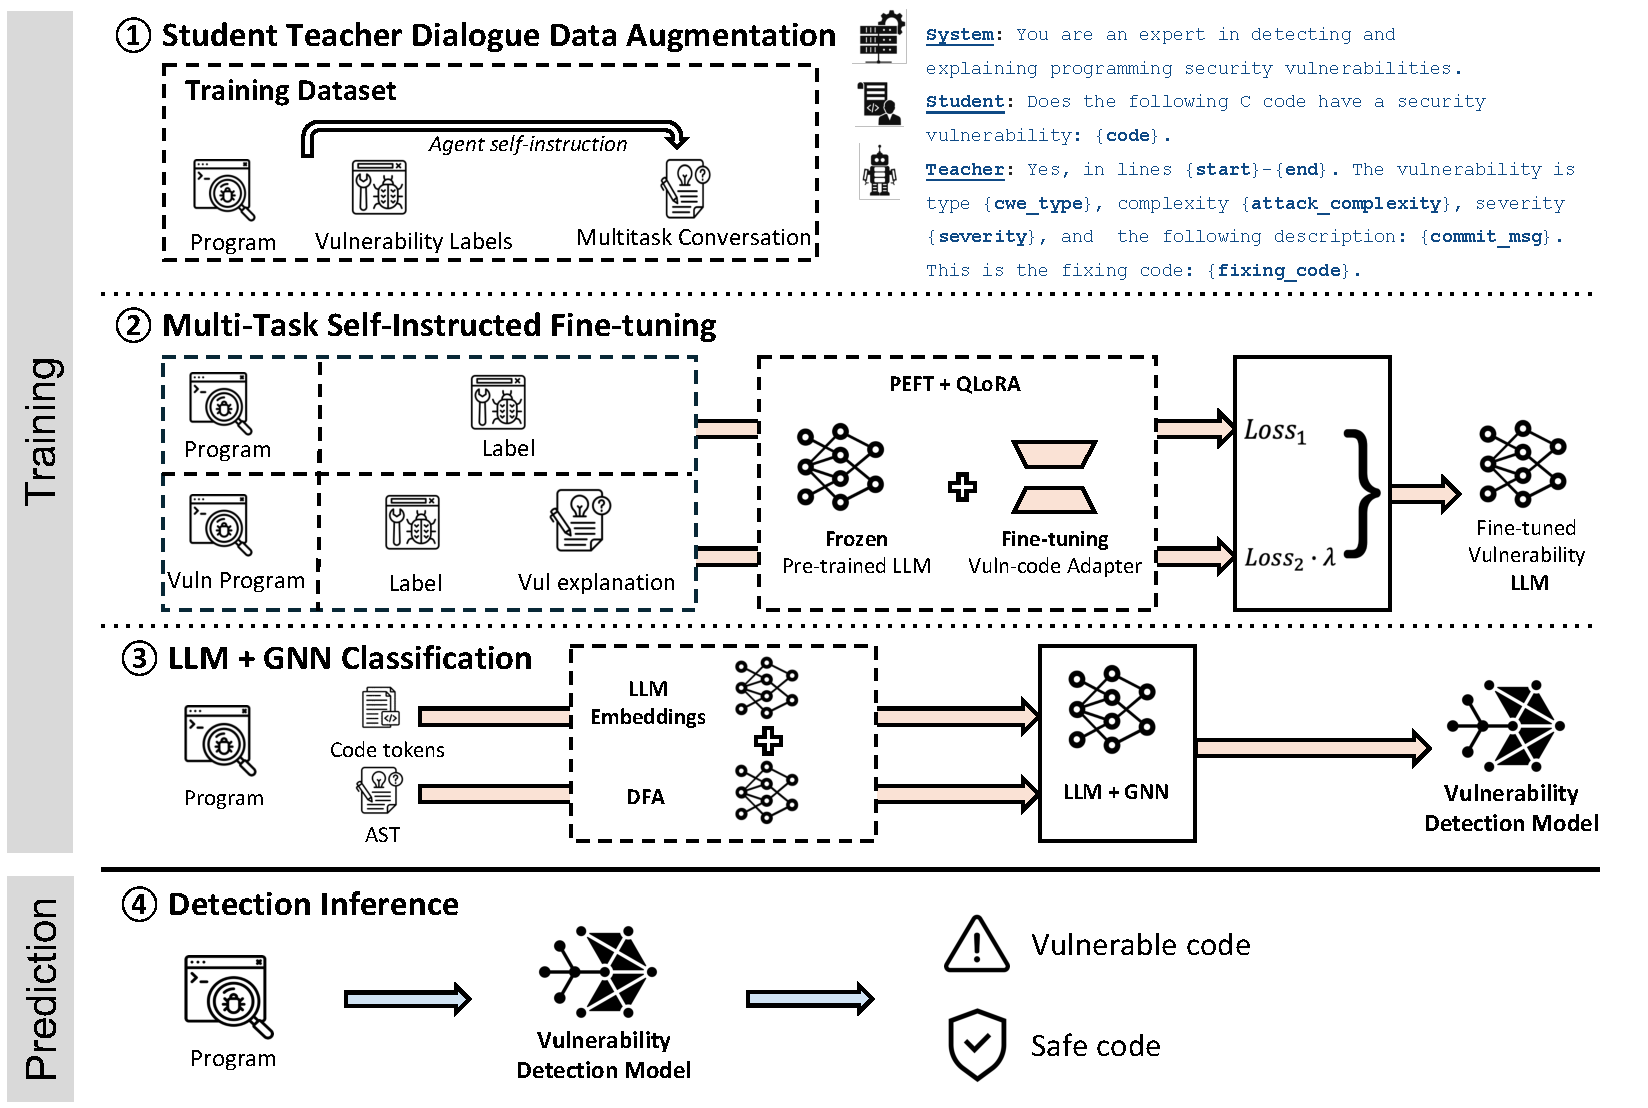
\includegraphics[width=\textwidth]{figures/approach/Multitask-vuln.pdf}
\caption{\small \textit{MSIVD}’s architecture, which takes as training data a code snippet, its vulnerability label, and various human annotated vulnerability labels. \textit{MSIVD} outputs a final vulnerability classification on unseen code snippets.}
\label{fig:multivuln_overview}
\end{figure*}

\section{MSIVD}

Figure~\ref{fig:multivuln_overview} provides an overview of MSIVD. The first three phases constitute training; the fourth phase, inference/vulnerability detection.
The design rationale behind \textit{MSIVD} is multi-faceted.  

First, because security vulnerabilities are fundamentally complex, 
vulnerability reports and curated datasets include multi-dimensional information, e.g., textual categorization and explanations, implicated code, potential fixes, and static analysis reports.  
I aim to leverage these diverse types of \emph{rich data} for training. 
During \textcircled{1} self-instruct dialogue-based data augmentation, \textit{MSIVD} prepares a given dataset for fine-tuning by extracting vulnerability characteristics including type, description, and source code location. 
The second step, \textcircled{2} multi-task fine-tuning, then uses multi-task learning to fine-tune an LLM towards two learning objectives:
(1) detecting a vulnerability and (2) providing an explanation that describes its characteristics. We focus on using \textit{MSIVD} for vulnerability detection, and leave an evaluation (i.e., a human study) of the quality of produced explanations to future work. However, we predicate \textit{MSIVD} on this type of multitask learning, including the explanation objective, because doing so can allow a model to simultaneously learn shared knowledge and patterns, improving generalization and accuracy. 
I overcome the small size of the available security vulnerability datasets
by taking advantage of recent LLM advances that enable lightweight, parameter efficient~\cite{peft}, and quantized adapter level fine-tuning~\cite{Llmao} suitable for smaller training datasets. 
Although these first two steps incorporate some code-level information, security vulnerabilities often entail specific, non-local, and subtle information flow.  
To reason about deeper semantic information, 
\textcircled{3} LLM+GNN training, jointly trains the LLM with a GNN based on information flow data derived from the program's control flow graph. 
This step represents the program as a graph, allowing the fine-tuned LLM to reason directly about 
whether the values and
data relations in a program indicate the occurrence of a vulnerability. 
In the \textcircled{4} detection phase, given a program, the vulnerability detection LLM trained by \textit{MSIVD} predicts whether a program contains a vulnerability.


\subsection{Data Augmentation}
To achieve security vulnerability detection incorporating vulnerability explanations, we first curated a custom dataset for both training and evaluating. The original dataset I use include samples of code snippets, and manually labelled classification on whether or not it includes a security vulnerability. The augmented dataset must allow the LLM to perform chain-of-thought, reasoning based on Self-instruct and Dialogue-policy-planned training. Therefore, the datapoints in our augmented vulnerability dataset must include a code snippet, its associated vulnerability label, CWE-type, a vulnerability description (e.g., how an attacker could exploit the vulnerability), and developer fix with fix location. 

I transform a classification based security vulnerability dataset into a suitable dialogue, enabling a multi-round conversation format between a teacher and student. 
Inserting intermediate reasoning steps like this improves the ability of an LLM to perform complex reasoning. Each complete dialogue is a single training data entry. Embedded with the conversation is first a system prompt asserting that the teacher is ``an expert in detecting and explaining programming security vulnerabilities'', followed by a back-and-forth of questions and answers about the vulnerability and its associated information.
Figure~\ref{code:dialogue} shows a complete dialogue training data entry example. The teacher and student converse in three rounds of dialogue, each on a different aspect of the security vulnerability in a target code snippet. The first round of dialogue discusses the existence of the vulnerability; the second round, an explanation of why the code snippet has a vulnerability; and the third, which lines need to be changed to fix the vulnerability.


\begin{figure*}[t!]
\centering
\begin{lstlisting}[numbersep=5pt,xleftmargin=21pt,numberstyle=\scriptsize,basicstyle=\footnotesize\ttfamily,firstnumber=1, language=C, language=C]
Round 0 = {
  role: "System",
  content: "You are an expert in detecting and locating security vulnerabilities, and can 
    help answer vulnerability questions", 
},
Round 1 = {
  role = "Student",
  content = f"Does the following code have any security vulnerabilities: {code_snippet}",

  role = "Teacher",
  content = f"Yes. The following code has a vulnerability type {cwe_type}.",
},
Round 2 = {
  role = "Student",
  content = f"What is the vulnerability description?",

  role = "Teacher",
  content =f"The vulnerability is:{commit_msg}",
}    
Round 3 = {
  role = "Student",
  content = f"Locate the lines that are vulnerable and should be repaired.",

  role = "Teacher",
  content = f"The code is vulnerable at lines {vuln_lines}, with the following fix: {fixing_code}",
}
\end{lstlisting}
\vspace*{-2mm}
\caption{\small A single training data entry for  the vulnerability detection multi-task fine-tuning. The dialogue rounds follow the four types of labelled data: vulnerability classification label,  description, type, and repair lines. 
}
\label{code:dialogue}
\end{figure*}

\subsection{Model setup}
I  train two models for \textit{MSIVD}. The first performs a sequence-to-sequence fine-tuning of a selected pre-trained LLM, using our multitask self-instruct approach. The second performs a sequence-to-classification training loop that outputs a binary classification label (i.e., if the sample is vulnerable or not), which we build on top of DeepDFA's GNN architecture.
The second model takes the final hidden states from the frozen in place first model. We refer to the tool using both models as \textit{MSIVD} throughout evaluation; the tool consisting only of the first model, without the GNN architecture, as \textit{MSIVD-}.  \textit{MSIVD-} converts the first model into a sequence-to-classification model directly, using a single \lstinline{linear} layer.
For the initial pre-trained model, we use CodeLlama-13B-Instruct~\cite{codellama}, which is the 13 billion parameters instruction tuned version of CodeLlama. CodeLlama released 4 model size versions, from 7B to 70B. Due to limited computing and VRAM, we chose the 13B version. 
Table~\ref{table:hyperparams_vuln} shows the hyperparameters used for both models. The 4352 model dimension from the LLM-GNN model is a result of concatenating the fine-tuned LLM (4096) with the GNN model (256). Similarly, we add the output layers of LLM with the GNN to form $8 + 3 = 11$ layers.
For batch size, we use 4 to fit CodeLlama 13B onto a single RTX 8000 GPU. However, other GPUs with more VRAM could employ higher batch sizes for greater efficiency. All experients used an Intel(R) Xeon(R) 6248R CPU @ 3.00GHz running Debian GNU/Linux 1 and two Nvidia Quadro RTX 8000 GPUs.




\begin{table}[t]
\centering
\caption{\small Hyperparameters for multitask self-instruct fine-tuning, and LLM-GNN combined vulnerability detection model training.
}
\begin{tabular}{l|rr}
\toprule
\textbf{Hyperparameter} & Multitask FT & LLM+GNN \\
\midrule
Initial Learning Rate  &  1e-5 &  1e-6\\
Model Dimension & 4096 & 4352\\
Context Window & 2048 & 2048 \\
Layers  &  8 & 11\\
Batch Size & 4 & 4 \\
Epochs & 10 & 5 \\
\bottomrule
\end{tabular}
\label{table:hyperparams_vuln}
\end{table}

\section{Evaluation and Results}

In this section, we present the results evaluating \textit{MSIVD}'s performance by answering three research questions:


\begin{enumerate}[leftmargin=3em]
    \itemsep0em 
    \item[\textbf{RQ1:}] How effective is \textit{MSIVD} at finding vulnerabilities on an established dataset?
    \item[\textbf{RQ2:}] To what extent can \textit{MSIVD} generalize to known-unseen vulnerabilities?
    \item[\textbf{RQ3:}] How does each component of \textit{MSIVD}, or vulnerability type, impact performance?
\end{enumerate}
All results presented in this section were obtained using an Intel(R) Xeon(R) 6248R CPU @ 3.00GHz running Debian GNU/Linux 1 and two Nvidia Quadro RTX 8000 GPUs.


\subsection{Setup}
\label{sec:baselines}

For classification, we convert the existence of a vulnerability into binary labels. To characterize classification effectiveness for an entire
dataset, we use F1, precision, and recall, following the same metrics used for the prior work~\cite{deepdfa, ivdetect, linevul, vuldeepecker}.

Security vulnerability detection has a rich research history long pre-dating recent advances in machine learning.
We focus our empirical comparison on work that uses machine learning for static vulnerability detection, as the recent results are especially promising, including compared to older, non-ML-based approaches. 
We compare \textit{MSIVD} to techniques that target general vulnerability detection (that is, not restricted to particular rule-sets or vulnerability types) at the same granularity level (the function level),\footnote{This granularity choice excludes several recent techniques, like Vuddy~\cite{vuddy}, VulChcker~\cite{vulchecker}, and LineVD~\cite{linevd}; these are statement-level.} and that either provide replication packages that can be applied to \textit{BigVul}, or include evaluation results on \textit{BigVul} in the original publication.  
Our chosen baselines cover several categories:

\begin{itemize}[leftmargin=5mm]
\item\emph{\textbf{Non-LLM} deep learning-based vulnerability detection tools}
VulDeePecker~\cite{vuldeepecker}, SySeVR~\cite{codet5}, Draper~\cite{draper}, IVDetect~\cite{ivdetect}, and DeepDFA~\cite{deepdfa}.
\item\emph{\textbf{LLM}-based approaches}, including (1) the vulnerability detection capabilities of open-source, pre-trained LLM models CodeBERT~\cite{codebert}, CodeT5~\cite{codet5}, and CodeLlama~\cite{codellama} (code pre-trained version of Llama-2), and (2) LineVul~\cite{linevul}, which trains an additional sequence-classification model on top of a pre-trained LLM. Although LineVul originally uses CodeBERT and RoBERTA~\cite{roberta} as its pre-trained LLM, we customize it to use the same pre-trained model (CodeLlama-13B) as \textit{MSIVD} and train for the same number of epochs (5). Otherwise, differences between \textit{MSIVD} and LineVul could be a due to differences in pre-trained model effectiveness, rather than approach.
\item\emph{\textbf{LLM + GNN} combined techniques} using DeepDFA's   replication package to combine their GNN embeddings with our fine-tuned model, as well as any HuggingFace pre-trained model directly. We train the same number of epochs (5) as \textit{MSIVD}.
\item\emph{\textbf{Random}} baseline that predicts whether a sample is vulnerable with a probability of 0.5, to ground precision, recall, and F1, whose performance is sensitive to the underlying data distribution (and our datasets are imbalanced).  
\end{itemize}

Our chosen baselines represent the state-of-the-art of vulnerability detection
models~\cite{deepdfa}, and all can be evaluated on the the \textit{BigVul} dataset.
Prior techniques relying on extant program analysis results cannot be trivially evaluated on the \textit{PreciseBugs} dataset; we therefore only evaluate the best-performing LLM-based techniques on it. 

\begin{table}[t!]
  \centering
\caption{\small Vulnerability prediction effectiveness on the Bigvul dataset. VulDeePecker, SySeVR, Draper, and IVDetect performance are from ref~\cite{ivdetect}, and CodeBERT and CodeT5 performance from ref~\cite{deepdfa}.
}
\begin{tabular}{l|lrrr}
\toprule \textbf{Type} & \textbf{Technique} &
 \textbf{F1} & \textbf{Precision} & \textbf{Recall}\\
\midrule

\multirow{1}{*}{Random} &
Random & 0.11  & 0.06  & 0.50   \\
\cmidrule{1-5}

\multirow{4}{*}{\parbox{0.9cm}{Non-LLM}}
& VulDeePecker & 0.12  & 0.49  & 0.19   \\
& SySeVR & 0.15  & 0.74  & 0.27   \\
& Draper& 0.16  & 0.48 & 0.24   \\
& IVDetect& 0.23  & 0.72 & 0.35   \\
& DeepDFA & 0.67  & 0.54 & 0.90   \\
\cmidrule{1-5}

\multirow{3}{*}{LLM}
& CodeBERT              & 0.21  & 0.68  & 0.13   \\
& CodeT5               & 0.46  & 0.56  & 0.39   \\
& CodeLlama            & 0.74  & 0.85  & 0.63 \\
& LineVul  & 0.81  & 0.86  & 0.78   \\
\cmidrule{1-5}
\multirow{2}{*}{LLM + GNN}
& CodeT5 + DeepDFA    & 0.79  & 0.85  & 0.71   \\
& LineVul + DeepDFA  & 0.88  & 0.88  & 0.89   \\
& \cellcolor{black!25} \textit{MSIVD}   &  \textbf{0.92} &  \textbf{0.93} &\textbf{ 0.91 }  \\


\bottomrule
\end{tabular}
\label{table:multift_results}
\end{table}

\subsection{Results}

\subsection{RQ1: Effectiveness on established dataset}
\label{sec:rq1}
Table~\ref{table:multift_results} shows the effectiveness of \textit{MSIVD}, and all baselines, on the \textit{BigVul} dataset. 
DeepDFA's data flow analysis-based GNN technique outperforms prior non-LLM techniques, with a F1 score of 0.67, largely due to its high recall of 0.9  (correctly identifying 90\% of the vulnerable code samples).
However, Table~\ref{table:multift_results} also shows that \emph{all} LLM approaches other than CodeBERT outperform all non-LLM approaches. That is, LineVul, without any insights from program analysis, surpasses all state-of-the-art program-analysis-based deep learning tools, although it is even more effective when combined with DeepDFA's GNN layers. 
Model knowledge from static analysis provides limited improvement for more powerful LLMs like CodeLlama; this knowledge more clearly benefits more dated LLMs like CodeT5 (i.e., F1 score improving from 0.46 to 0.79). 
Overall, \textit{MSVID} achieves F1 of 0.92, precision 0.93, and recall 0.91, outperforming all baselines on all metrics. These results demonstrate that the different aspects of vulnerability explanation can indeed improve a pre-trained LLM's vulnerability detection accuracy. However, \textit{MSVID} only shows incremental improvements over LineVul + DeepDFA, as compared to LineVul + DeepDFA's larger improvements over all non-LLM tools. The largest improvements on vulnerability detection with the \textit{BigVul} dataset comes from the underlying LLM itself. 

\begin{tcolorbox}
[colback=white,colframe=black,arc=0pt,boxrule=0.5pt,title=RQ1 Summary,boxsep=2pt,left=1pt,right=1pt,top=1pt,bottom=1pt,fonttitle=\bfseries] 
LLM-based techniques outperform non-LLM techniques on the \textit{bigvul} dataset. \textit{MSVID} outperforms prior all state-of-the-art approaches, with an F1 score of 0.92. The incremental improvements of adding either GNNs or fine-tuning suggests that the underlying pre-trained LLM is capable of effective vulnerability prediction based on code tokens alone.
\end{tcolorbox}

\subsection{RQ2: \textit{MSIVD} effectiveness on unseen vulnerabilities} 
\label{sec:rq2}

Table~\ref{table:multift_results} shows \textit{MSIVD}-'s performance on the \textit{PreciseBugs} dataset, comparing to LineVul (the best-performing prior technique on \textit{BigVul}). \textit{MSIVD} shows a larger improvement over LineVul on the newer dataset (F1 of 0.48 to LineVul's F1 of 0.31) as compared to on \textit{BigVul}.  This demonstrates the relative effectiveness of our fine-tuning approach on unseen vulnerabilities.

We sought to understand why LineVul with CodeLlama as the underlying model performs so much worse on \textit{PreciseBugs} than on \textit{BigVul}. 
One clue lies in CodeLlama's effectiveness on our evaluation data  on its own: Table~\ref{table:multift_results} shows that CodeLlama achieves an F1 score of 0.74 on \textit{BigVul}, but only 0.22 on \textit{PreciseBugs}. Without any additional vulnerability classification training or sequence-to-sequence fine-tuning, CodeLlama already beats most prior non-LLM techniques.

More telling evidence emerges from the training loss function for CodeLlama using our multitask fine-tuning method.
A deep-learning model's loss curve describes how closely a model's predictions are to the ground truth.  We expect loss to generally decrease as training epochs increase; lower loss means better prediction. 
Figure~\ref{fig:loss} shows the loss curves of our training approach on the \textit{BigVul} dataset with (i.e., multitask  fine-tuning) and without explanations (i.e., label-only fine-tuning).
The loss curve on fine-tuning \textit{BigVul} with explanation approaches 0.2 in 400 steps (2 epochs, roughly 16 hours of training time).
In contrast, the loss curve on fine-tuning \textit{BigVul} without explanations approaches 0.2 in 50 steps (1/4 of an epoch, roughly 2 hours of training time). 
Near-zero loss, with minimal training, is a strong indication of data leakage and overfitting.  Here, the pre-trained LLM (CodeLlama) shows clear over-fitting (i.e., prior memorization of the dataset) on \textit{BigVul} without explanations.  Adding explanations includes more information, and adding non-binary labelling naturally induces noise, explaining why fine-tuning with explanations is not as overfit. 
Note that we observe the same loss curve behavior on the \emph{Devign} dataset, using the same setup (not shown). 
This suggests that much of the accuracy of LLM-based techniques is likely arises from dataset memorization. This supports the importance of evaluating LLM-based approaches on labelled vulnerabilities collected after the selected LLM's training data cut-off date. Our results also demonstrate the value of fine-tuning LLMs using a multitask approach which, even on previously seen data, inserts a useful degree of randomness in learning.



\begin{figure}
\centering
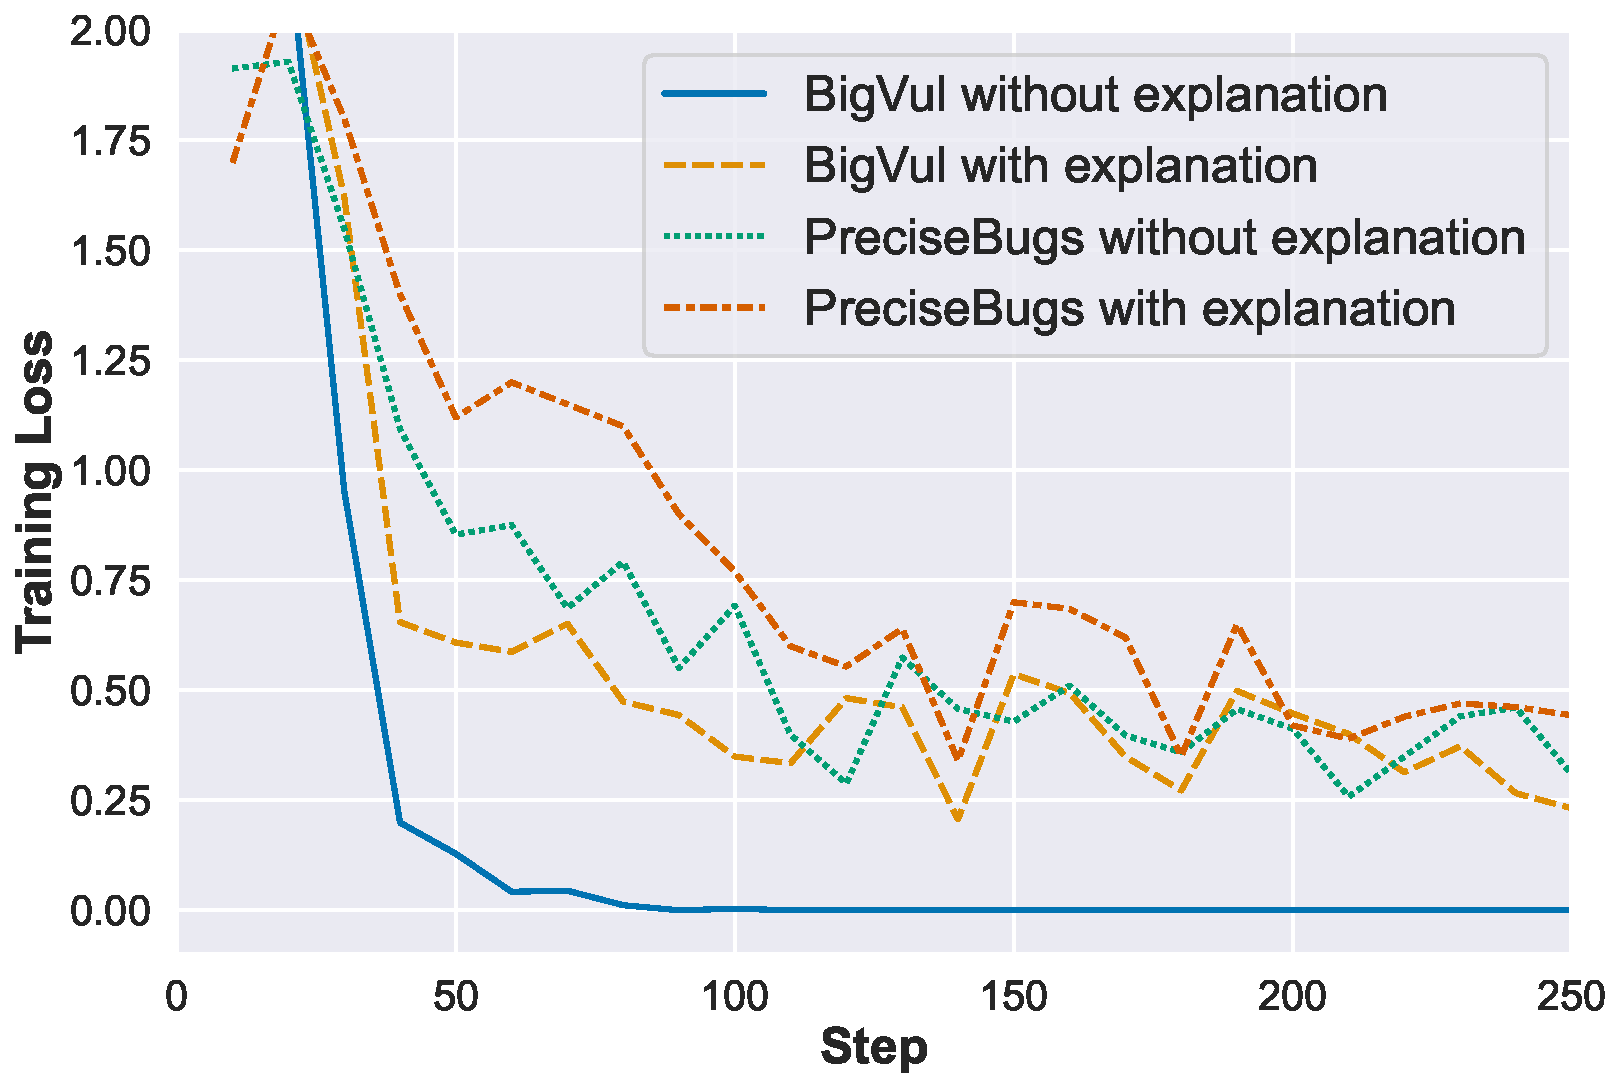
\includegraphics[width=0.7\columnwidth]{figures/results/train_loss.pdf}
\caption{\small Loss curve of \textit{MSIVD} fine-tuning CodeLlama for \textit{BigVul} and \textit{PreciseBugs}. Lower loss indicates model predictions closer to the ground-truth labels. Near-zero loss, with minimal training, indicates over-fitting~\cite{overfitting}. Note that the pre-trained LLM (CodeLlama) shows obvious over-fitting on \textit{BigVul} without explanations, motivating the necessity for new labelled datasets for model evaluation.
}
\label{fig:loss}
% \Description{loss}
\end{figure}



\begin{tcolorbox}
[colback=white,colframe=black,arc=0pt,boxrule=0.5pt,title=RQ2 Summary,boxsep=2pt,left=1pt,right=1pt,top=1pt,bottom=1pt,fonttitle=\bfseries]
Neither CodeLlama alone nor prior LLM-based vulnerability detector baselines generalize well to the unseen \textit{PreciseBugs} dataset. Training loss curves suggest that CodeLlama has likely memorized the \textit{BigVul} dataset. While \textit{MSIVD} is therefore more effective on \textit{BigVul} than on \textit{PreciseBugs} vulnerabilities, it better generalizes to the recently released \textit{PreciseBugs} dataset than the prior baselines. 
\end{tcolorbox}

\subsection{RQ3: Ablation study}
\label{sec:rq3}


\noindent\textbf{Setup.} To answer RQ3, we evaluate \textit{MSIVD} under four settings and evaluate their performances on \textit{BigVul} and \textit{PreciseBugs}. First, we use the underlying pre-trained LLM directly for prediction (as in \textit{RQ1}). We then use a fine-tuned version of \textit{MSIVD}, but without any vulnerability explanations in its training data (label-only FT). Finally, we include vulnerability explanations in a single round of self-instruction fine-tuning (single-round SIFT) and multiple rounds of self-instruction fine-tuning (multi-round SIFT, which corresponds to \textit{MSIVD}-). For \textit{BigVul}, we also add the GNN adapter layers (multi-round SIFT + GNN, which corresponds to the full version of \textit{MSIVD}). 

We additionally evaluate our tool on specific vulnerability types within \textit{PreciseBugs}, (training/evaluating on single vulnerability types). We choose the three most common types from our \textit{PreciseBugs} dataset: buffer error (27.3\% of \textit{PreciseBugs}), resource error (21.2\% of \textit{PreciseBugs}), and input validation error (13.6\%). 

\noindent\textbf{Results.} Table~\ref{table:multift_ablation} shows results on both the \textit{BigVul} and \textit{PreciseBugs} datasets. As discussed in Section~\ref{sec:rq2}, CodeLlama already performs well at detecting \textit{BigVul} vulnerabilities. Training a separate model without using agent self-instruction slightly improves effectiveness, with a F1 score of 0.81 (+0.07 above the pre-trained F1 score of 0.74) for \textit{BigVul}, and a F1 score of 0.33 (+0.1 above pre-trained) on \textit{PreciseBugs}.

Surprisingly, we find that fine-tuning on only the vulnerability label and none of the explanations actually performs worse than using a pre-trained model directly for vulnerability classification (0.71 F1 for fine-tuned CodeLlama, and 0.74 F1 for pre-trained CodeLlama on the \textit{BigVul} dataset). 
Our findings are consistent with those of Yusuf et al.~\cite{instruct_vul}, who observed that instruction-based fine-tuning may not always enhance performance, especially across a dataset of diverse CWEs. The shift from sequence-to-sequence fine-tuning to the sequence-classification training within a small dataset may simply include more noise, reducing classification performance.

Fine-tuning with both code and vulnerability explanations with the multitask agent setup (\textit{MSIVD}) yields the highest vulnerability detection on both \textit{BigVul} and \textit{PreciseBugs}. 
We also see that training with multi-round SIFT yields higher F1 scores than single-round SIFT (a F1 improvement of 0.09 for \textit{BigVul}, and 0.02 for \textit{PreciseBugs}), which is consistent with prior work on LLM instruction-prompting~\cite{zero-shot}. Finally, we observe that the additional GNN (multi-round SIFT + GNN) provides an additional 0.02 F1 on top of multi-round SIFT for the \textit{BigVul} dataset. The incremental improvement from the addition of GNN shows that CodeLlama already makes accurate predictions based on prior knowledge on the \textit{BigVul} dataset, as previously discussed in Section~\ref{sec:rq2}.

\begin{table}[t!]
  \centering
\caption{\small \textit{MSIVD} ablation study. ``Pre-trained" uses the underlying LLM directly for vulnerability detection. ``Label-only fine-tuned'' (FT) performs single-task fine-tuning on the vulnerability classification labels. ``Single round self-instruct fine-tuned (SIFT)'' trains the LLM without the agent explanation multi-round dialogue. ``Multi-round SIFT'' uses multi-task agent-dialogue fine-tuning (\textit{MSIVD}$^{-}$). ``Multi-round SIFT + GNN'' adds the GNN adapter layer and corresponds to the full version of \textit{MSIVD}.
}

\begin{tabular}{l|lrrr}
\toprule
 \textbf{Dataset} & \textbf{Technique} &
 \textbf{F1} & \textbf{Precision} & \textbf{Recall}\\
\midrule
\multirow{3}{*}{\textit{BigVul}}
& Pre-trained & 0.74  & 0.85  & 0.55   \\
& Label-only FT & 0.71 & 0.77  & 0.66    \\
& Single-round SIFT & 0.81  & 0.86  & 0.61   \\
& Multi-round SIFT      & 0.90  & 0.91  & 0.87 \\
& \parbox{2cm}{Multi-round SIFT + GNN} & 0.92  & 0.93 & 0.91   \\
\midrule

\multirow{3}{*}{\textit{PreciseBugs}}
& Pre-trained & 0.22  & 0.16  & 0.35   \\
& Label-only FT & 0.31  & 0.43  & 0.25   \\
& Single-round SIFT & 0.33  & 0.46  & 0.25   \\
& Multi-round SIFT  & 0.48  & 0.4   & 0.57\\
\midrule
\multirow{3}{*}{\parbox{2cm}{\textit{PreciseBugs} Vuln. Type}}
& \textit{MSIVD}minus Input  & 0.46  & 0.49   & 0.44    \\
& \textit{MSIVD}minus Resource  & 0.58  & \textbf{0.63}   & 0.51    \\
& \textit{MSIVD}minus Buffer  &\textbf{ 0.59}  & 0.62   & \textbf{0.57 }   \\


\bottomrule
\end{tabular}
\label{table:multift_ablation}
\end{table}


Table~\ref{table:multift_ablation} shows that training and evaluating on single vulnerability types improves F1 scores as compared to the entire dataset, but by trading off higher precision for lower recall. 
These results further corroborate that the LLM-unseen vulnerabilities in the newer \textit{PreciseBugs} dataset are more difficult for any language model to detect. However, our results also indicate that training with a multi-round self-instruct format on a dataset with both label and explanation produces considerable improvements over pre-trained models alone, and substantiate the value of the individual components of \textit{MSIVD}'s design. 

\begin{tcolorbox}
[colback=white,colframe=black,arc=0pt,boxrule=0.5pt,title=RQ3 Summary,boxsep=2pt,left=1pt,right=1pt,top=1pt,bottom=1pt,fonttitle=\bfseries]
Further training a code LLM on vulnerability-specific code and labels improves detection effectiveness. Fine-tuning an LLM without vulnerability explanations actually reduces effectiveness as compared to the pre-trained model alone. Multitask fine-tuning with all included vulnerability explanations achieves the highest detection effectiveness, especially with multiple rounds of self-instruction. Finally, selecting specific vulnerability types for both training and evaluating yields higher F1 scores, but with a trade-off of lower recall due to the smaller data size.
\end{tcolorbox}

\section{Conclusion}
Automatically detecting software security vulnerabilities is a rich and longstanding problem. Recent advances in ML have enabled techniques to combine program analysis with deep learning or LLMs.
Meanwhile, the relatively small curated security vulnerability datasets provide rich additional information that prior work has left unexplored. We bridge this gap by introducing a self-instruct based multitask fine-tuning model to learn vulnerability classification based on both program code and vulnerability explanations. We further include information from data flow analysis, and build a light-weight GNN adapter based on a program's call graph to achieve simultaneous transfer-learning between LLM and GNN. 
Our tool surpasses prior state-of-the-art results on established vulnerability datasets. Furthermore, because of the risk (and evidence) of LLM data contamination, we collect a novel vulnerability dataset with evaluation and test samples  exclusively filtered to be vulnerabilities identified past our pre-trained code LLM's training cutoff, and show that our technique outperforms prior work on that dataset as well. 

\chapter{Node.js Vulnerability Detection with Program Analysis and pretrained LLMs}

As discussed in Chapter~\ref{ch:msivd}, we aim to improve the vulnerability detector from Chapter~\ref{ch:llmao} for larger, real-world repositories. Chapter~\ref{ch:msivd} extends \textit{LLMAO} with \textit{MSIVD}, which addresses the key limitation of context window sizing. \textit{MSIVD} leverages the data flow analysis (DFA) of a program into trainable objectives for LLM-based vulnerability detection. DFA tracks how data moves through program variables by capturing control flow and data dependencies. However, not all information passed across a repository is represented by variables. A more specific static analysis technique is the creation of \textit{provenance graphs}. Provenance graphs track data origins and transformations, and focuses on capturing relationships between data artifacts and processes. Provenance graphs investigate the ``why'' and ``how'' of data transformations, which are necessary for uncovering certain exploits. In this work, we further extend our previous vulnerability detector with provenance graphs, which are constructed through dynamic taint analysis that capture the
complete history of operations applied to tainted values during a program’s execution. Each node in a provenance graph represents a taint-related operation or value, while edges illustrate the flow of data between these nodes.

The popular Node.js ecosystem has become an attractive target for attackers. Two of the most serious vulnerabilities are Arbitrary Command Injection (ACI) and Arbitrary Code Execution (ACE), which allow attackers to execute malicious commands or code on the system that runs the application. Prior work such as \nodemedicfine used program synthesis to generate proof-of-concept exploits for Node.js packages for vulnerability confirmation. However, there are many instances where no exploit is produced, resulting in a high number of false positives that require manual analysis. 

This work investigates whether ML-based approaches can predict ACE and ACI vulnerabilities in Node.js packages. We present a large-scale dataset of over 2,000 package-level vulnerabilities with human-reviewed labels. We conduct a comprehensive evaluation of approaches based on large language models (LLMs), program analysis extended with ML approaches, and hybrid ML methods.
We integrate the vulnerability detection engine of a prior program analysis tool, \nodemedic, with Graph Neural Networks, Random Forest, XGBoost, Logistic Regression, SVM, and LLMs to reduce false negatives.

Our results indicate that 
both traditional machine learning models and LLMs when combined with program analysis tools can predict Node.js package exploitability with high accuracy.
Our work provides insights into the effectiveness and challenges of using LLMs for vulnerability detection in JavaScript packages.

\section{NODEMEDIC-LLM}
In this work, we conduct a comprehensive evaluation of LLM-based methods, program analysis-based methods, ML-enhanced program analysis methods, and a hybrid approach that combines LLMs, \nodemedicfine, and GNNs for detecting vulnerabilities in JavaScript code.
A summary of our approaches is shown in Figure~\ref{fig:nodemedic}.
More concretely, we implement the following approaches with machine learning predictors that can help reduce the effort required for manual confirmation of package exploitability. (1) LLMs that do not rely on program analysis tools. (2) \nodemedic{-ML} that applies various ML models (Random Forest, XGBoost, Logistic Regression, and SVM) to predict vulnerabilities based on the provenance graph output from the dynamic taint analysis tool \nodemedicfine. 
(3)\nodemedic{-GNN}, which is setup similarly as \nodemedic{-ML} but uses Graph Neural Networks. 
(4) \nodemedic{-GNN-LLM}, which combines the embedding layers of the GNN model and the pre-trained language models (LMs).


\subsection{Dataset}\label{subsec:datasets}
The dataset used for our evaluation consists of 2,051 npm packages in which \nodemedicfine identified potential vulnerable calls to sinks. These packages were selected from a total of 33,011 npm packages analyzed for ACI and ACE vulnerabilities by \nodemedicfine and shared by the authors of \nodemedicfine.

Of the 2,051 potentially vulnerable npm packages, 1,465 have been confirmed to be vulnerable with working exploits. Of these, 728 were automatically confirmed by \nodemedicfine, while 737 were confirmed manually. 

Since LLM methods, the LLM-GNN hybrid method, and ML-enhanced \nodemedicfine methods require parts of the data for training and validation, we randomly divided the 2,051 package dataset into three subsets (train, validation, and test) in an 8:1:1 ratio. The training set includes 1,640 packages, the validation set includes 205 packages, and the testing set includes 206 packages.
For models requiring training, the training set is used to train the model, while the validation set is used to select the best model model before evaluation. All models are then evaluated on the same testing set to ensure consistent performance reporting.
Table \ref{tab:dataset-overview} provides a detailed overview of these dataset splits.

\begin{figure*}[t]
    \centering
    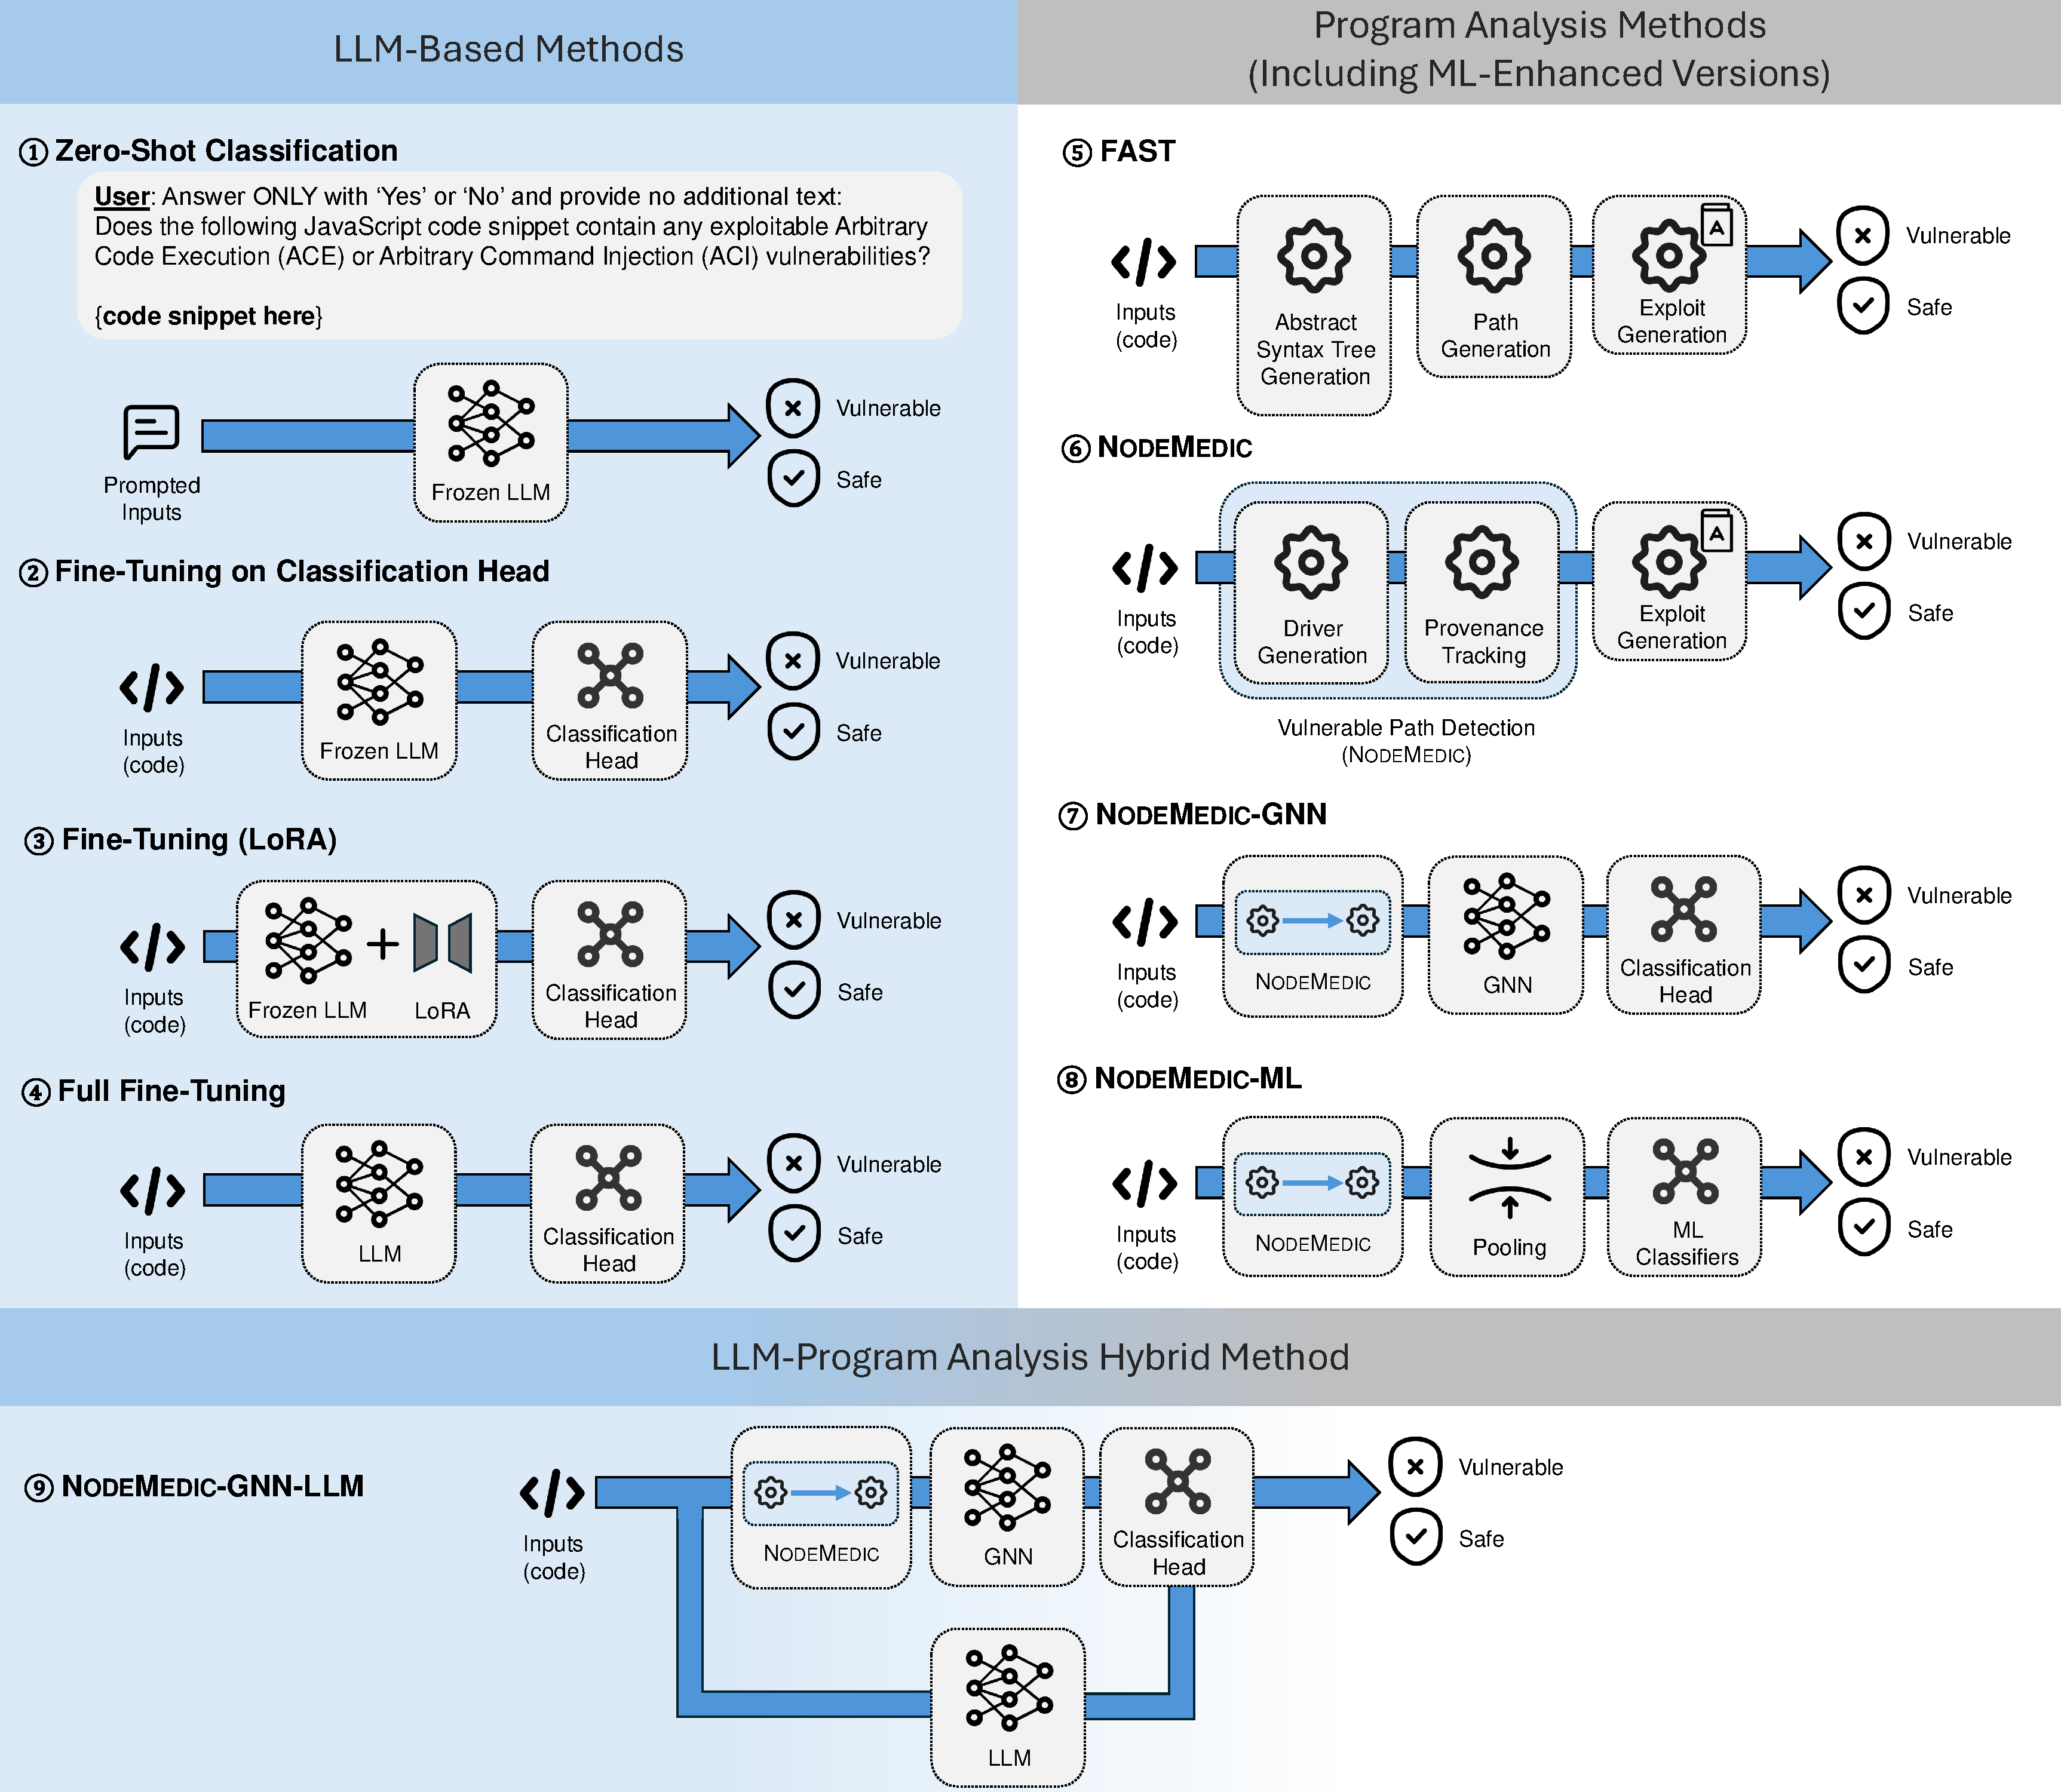
\includegraphics[width=0.9\textwidth]{figures/approach/nodemedic.pdf}
    \caption{Nodemedic-LLM vulnerability detection approach}
    \label{fig:nodemedic}
\end{figure*}


\begin{table}[t]
\centering
\caption{Overview of the dataset splits used in the evaluation. The table displays the total number of packages in each split (\textit{train}, \textit{validate}, and \textit{test}), along with the number of vulnerable packages in each split, categorized into ACE and ACI. Numbers in parentheses indicate the count of vulnerable packages within each split.
}
\label{tab:dataset-overview}
\begin{tabular}{|c|c|c|c|}
\hline
\textbf{Split} & \textbf{Total (Vuln)} & \textbf{ACE (Vuln)} & \textbf{ACI (Vuln)} \\ \hline
train & 1640 (1173) & 335 (290) & 1,305 (883) \\ \hline
validate & 205 (140) & 45 (38) & 160 (102) \\ \hline
test & 206 (152) & 40 (32) & 166 (120) \\ \hline
total & 2,051 (1,465) & 420 (360) & 1,631 (1,105) \\ \hline
\end{tabular}
\end{table}




\subsection{LLM-based Methods}
Common practices in leveraging large language models (LLMs) for vulnerability detection typically fall into two categories:
\begin{enumerate}
    \item \textbf{Zero-shot and few-shot prompting}, where the model is provided with code snippets along with carefully designed natural language queries to identify security risks. This approach benefits from LLMs' generalization ability but often struggles with nuanced vulnerabilities that require deeper program understanding.
    \item \textbf{Fine-tuning}, where the model is trained on labeled vulnerability datasets to learn domain-specific patterns. Fine-tuning can significantly improve detection accuracy but comes with high computational costs and data collection challenges. Other than full fine-tuning, there are also lightweight fine-tuning methods, such as LoRA fine-tuning \cite{lora, qlora} and fine-tuning on only selected layers.
\end{enumerate}

To systematically evaluate LLMs in vulnerability detection, we assess several models under different settings, including zero-shot classification, fine-tuning on a classification head, LoRA fine-tuning \cite{lora, qlora}, and full fine-tuning. We exclude few-shot learning in this work because the large input size of the code snippets makes it difficult to fit multiple samples into a reasonable context window.
The code snippet given to LLMs is the file that contains potential sinks. If the file is too long to fit within the predefined context length, we truncate it, taking code immediately around the sink. This is based on our observations that the majority of vulnerable logic is local to the sink and the surrounding code in the dataset. 

\subsubsection{Zero-Shot Classification \textup{(\ding{172} in Figure \ref{fig:nodemedic})}}
 
In this setting, we use an auto-regressive generation head that enables the LLM to generate a textual response indicating whether a given JavaScript package contains vulnerabilities. 
%
Zero-shot classification relies entirely on the LLM's pre-trained knowledge and ability to generate a relevant answer token by token in an auto-regressive manner.

For this evaluation, we prompt the LLM with a common query:
\begin{tcolorbox}[colback=gray!10, colframe=black, arc=3mm, boxrule=0.8pt]
    \textbf{User:} Answer ONLY with ‘Yes’ or ‘No’ and provide no additional text:\\
    Does the following JavaScript code snippet contain any exploitable Arbitrary Code Execution (ACE) or Arbitrary Command Injection (ACI) vulnerabilities?\\
    
    \texttt{\{code snippet here\}}
\end{tcolorbox}

For models that can run locally, we disable sampling during generation to ensure deterministic results. For some models that require a cloud-based API, the classification responses may vary slightly across multiple runs. 
Even though we instruct the model to output only "Yes" and "No," for models trained on a Chain-of-Thought (CoT) objective \cite{wei2022chain}, the model may still produce extra text wrapped in special tokens as part of the reasoning process before the final answer. We ignore these additional tokens and only consider the final answer.
%
The outputs are filtered based on the presence of ''Yes'' which is considered vulnerable, while all other cases, including those that generate neither "Yes" nor "No," are considered non-vulnerable.

\subsubsection{Fine-Tuning on a Classification Head \textup{(\ding{173} in Figure \ref{fig:nodemedic})}}

Instead of using a generation head, we attach a classification head on top of the base LLMs and fine-tune the model for the vulnerability detection task while keeping the base LLMs frozen (not involved in training). The classification head takes the embedding from the last non-padding position of the output from the last attention layer as input and produces an output shape of 2 logits, representing the two classes (vulnerable or non-vulnerable). We use the cross-entropy loss function to train the classification head with weights that correspond to the class imbalance in the dataset.

\subsubsection{LoRA Fine-Tuning \textup{(\ding{174} in Figure \ref{fig:nodemedic})}}

LoRA (Low-Rank Adaptation) fine-tuning \cite{lora, qlora} offers a lightweight approach to adapting LLMs without updating all parameters. Instead of modifying the entire model, LoRA injects low-rank adapters into selected layers of the model. These adapters are small, low-rank matrices that are learned during fine-tuning. Similar to the previous method, we attach a classification head on top of the base LLMs and fine-tune the model for the vulnerability detection task. However, in this case, we only update the low-rank adapters and the classification head, while the base LLMs remain frozen. The same cross-entropy loss function is used to train the classification head.

\subsubsection{Full Fine-Tuning \textup{(\ding{175} in Figure \ref{fig:nodemedic})}}

In full fine-tuning, we update all parameters of the LLM and the classification head using our labeled vulnerability dataset, applying the same cross-entropy loss function as previously described.

During the fine-tuning of all the aforementioned LLM-based methods, all frozen parameters are stored in 4-bit NormalFloat (NF4) precision for memory efficiency \cite{qlora}, while the trainable parameters are in 16-bit BrainFloat (BF16) precision.

\subsection{ML-enhanced Program Analysis Methods}

\nodemedic{-GNN} and \nodemedic{-ML} utilize \nodemedic's
taint provenance tracking component to create provenance graphs (as described in Section \ref{subsec:provenance-analysis}) in both the training and inference pipelines. The operation, tainted status, and sink type of each node are used as inputs. Additionally, the vulnerability type is included as an input for the entire graph. The 100 most common operations in our dataset (as described in Section 3.1) are assigned class numbers \texttt{0} to \texttt{99}. Class \texttt{100} is designated for less frequent operations, while class \texttt{101} is used for empty or missing operation attributes in the provenance graphs. Tainted statuses are encoded as class \texttt{0} for \texttt{False} (untainted), class \texttt{1} for \texttt{True} (tainted) and class \texttt{2} for missing attributes. Sink types are represented with class \texttt{0} for \texttt{spawn}, class \texttt{1} for \texttt{exec}, and class \texttt{2} for missing attributes. Vulnerability types are encoded as class \texttt{0} for ACE and class \texttt{1} for ACI vulnerabilities.

Each attribute is represented as a one-hot vector, where the corresponding class has a value of \texttt{1}, and all other classes have a value of \texttt{0}. The four one-hot vectors are then concatenated to form the embedding for a single node in the graph. Together, the graph's topology and the embeddings of its nodes make up the complete representation of the graph.

\subsubsection{\nodemedic{-GNN} \textup{(\ding{178} in Figure \ref{fig:nodemedic})}}

The GNN component in \nodemedic{-GNN} starts with a Gated Graph Sequence Neural Network (GGNN) \cite{li2015gated}, which is a specialized type of neural network designed to learn from graph-structured data by capturing dependencies and relationships between nodes. The GGNN works by iteratively passing messages along edges, enabling each node to gather information from its neighbors and update its representation based on the graph’s structure and features. In the final step, the learned abstract node embeddings are combined into a graph-level representation using Global Attention Pooling~\cite{li2015gated}, resulting in the final graph embedding. The graph embedding is then fed into a classification head to predict vulnerability.\sloppy



\subsubsection{\nodemedic{-ML} \textup{(\ding{179} in Figure \ref{fig:nodemedic})}}

In \nodemedic{-ML}, only the node embeddings of the graph are taken into account, while the topology is disregarded. The embeddings of all nodes are first fed into a pooling layer to create a unified shape embedding vector that represents the entire graph, regardless of the number of nodes. The pooled embedding is then passed through machine learning classifiers to predict the vulnerability.

\subsection{LLM-Program Analysis Hybrid Methods}

To bridge the gap between program analysis and LLM-based reasoning, we evaluate a hybrid approach \textup{(\ding{180} in Figure \ref{fig:nodemedic})} that combines \nodemedicfine{’s} vulnerability path detection, graph neural networks (GNNs), and large language models (LLMs). This method, referred to as NodeMedic-GNN-LLM , integrates the strengths of both program analysis and LLMs to enhance vulnerability detection. 

This hybrid approach uses the output from the GNN model and the output from the LLM as its embeddings. The two embeddings are concatenated and sent through a classification head to predict the vulnerability. The full model is trained end-to-end, with the GNN and LLM components updated simultaneously.


\section{Experiment Setup}
We first outline the model selection and implementation (Section \ref{subsec:model_selection}) used in our evaluation. Next, we discuss the evaluation metrics (Section \ref{subsec:experiment_metrics}) and the system configuration (Section \ref{subsec:system_config}).



\subsection{Model Selection and Implementation}\label{subsec:model_selection}

We directly report the latest results from the \nodemedicfine experiments in Section \ref{sec:results}. We evaluated FAST~\footnote{FAST implementation accessed at \url{https://github.com/fast-sp-2023/fast}}
against our dataset. For FAST, we enabled the \texttt{-X} flag to turn on auto-exploit generation. 
% \limin{this is covered in background}
% However, it is worth noting that FAST does not actually execute an exploit to confirm the vulnerability. Instead, it attempts to solve the exploitability constraints and reports a vulnerability as exploitable if a solution is found. 
Additionally, for FAST, we used the \texttt{-t} flag to specify vulnerability types as \texttt{os\_command} and \texttt{code\_exec}, which correspond to ACI and ACE vulnerabilities, respectively.


For \nodemedic{-ML}, we evaluate %several machine learning (ML) methods: 
logistic regression, support vector machine (SVM), random forest, and XGBoost. These methods are trained on provenance graphs generated by \nodemedicfine. For logistic regression, SVM, and random forest experiments, we used classes from the \texttt{scikit-learn} library, while the \texttt{xgboost} package was used for XGBoost experiments. For these machine learning baseline models, default hyperparameters were applied, and the random state was set to 42 for reproducibility.

For \nodemedic{-GNN}, we use the GatedGraphConv and GlobalAttentionPooling modules from the Deep Graph Library~\cite{wang2019deep}.

For the LLM-based methods, we experiment with 
% several large language models (LLMs) and their different pretrained versions. We use the following: 
DeepSeek-R1-Distill-Qwen-14B, DeepSeek-R1-Distill-Llama-8B, DeepSeek-R1-Distill-Qwen-7B \cite{deepseek2025deepseek}, Llama-3.1-8B-Instruct \cite{dubey2024llama}, Qwen2.5-Coder-14B-Instruct, and Qwen2.5-Coder-7B-Instruct \cite{qwen2.5}. We utilized the implementation and parameters of the models provided by Hugging Face. Additionally, we experiment with two models evaluated via cloud APIs: OpenAI o3-mini-high and DeepSeek-R1 \cite{deepseek2025deepseek}. The random state is set to 0 to ensure reproducibility.
For LoRA, we are using a rank of 256 and an alpha of 512 for all experiments. An ablation study on LoRA's hyperparameters is presented in Section \ref{subsec:rq4}.

\subsection{Evaluation Metrics}\label{subsec:experiment_metrics}

\nodemedicfine, FAST, and zero-shot LLM models are evaluated directly on the test dataset, while other models that require training are trained on the training dataset and validated on the validation dataset during the training process. The best model from training is then evaluated on the test dataset.
To assess the performance of each method, we employ the following metrics: $F1 = \frac{TP} {TP + 0.5(FP + FN)}$, $Precision = \frac{TP}{(TP + FP)}$, $Recall = \frac{TP}{TP + FN}$ (where TN is true negative, TP is true positive, FP is false positive, and FN is false negative).
These are the same metrics used for prior work on vulnerability detection~\cite{deepdfa, ivdetect, linevul, yang2024security}.

\subsection{System Configuration}\label{subsec:system_config}

Evaluations that require only CPUs are conducted on a computing cluster. Each task runs individually in a virtually isolated environment with a 2-core CPU, which is part of an AMD EPYC 7742 processor, and 16 GB of RAM. The timeout for each task is set to 36 hours. For experiments that require GPUs, except for those where LLMs are undergoing full fine-tuning, each task is executed in a virtual environment with one NVIDIA H100 (80GB) GPU, two Intel Xeon 8480C PCIe Gen5 CPUs (each with 56 cores running at 2.0/3.8 GHz), and 2 TB of RAM. For LLMs that require full fine-tuning, we use a computing cluster with four NVIDIA H100 (80GB) GPUs, two Intel Xeon 8480C PCIe Gen5 CPUs (each with 56 cores running at 2.0/3.8 GHz), and 2 TB of RAM. 



\section{Results}
\label{sec:results}
Our experiments aim to address the following research questions:
\begin{itemize}[left=0pt, label={}]
    \setlength{\itemsep}{0pt}
    \item \textbf{RQ1: Effectiveness of LLMs.} How effective are LLM-based methods in detecting exploitable vulnerabilities in \nodejs packages compared to traditional program analysis approaches and ML-enhanced program analysis methods?
    \item \textbf{RQ2: Cross-Method Prediction Comparison.} How do the predictions of graph-based models (e.g., GNN-enhanced \nodemedicfine) and LLM-based methods differ, and does their combination lead to improved vulnerability detection?
    \item \textbf{RQ3: Ablation Study on LLMs.} How do different large language models and usage strategies (e.g., zero-shot, various fine-tuning methods) perform in our vulnerability detection task?
    \item \textbf{RQ4: Training and Inference Time.} How do LLM-based methods compare to traditional program analysis approaches in terms of prediction latency and pre-prediction (training) time?
    
    % \item \textbf{RQ5:} What are the key challenges in using LLMs for package-level vulnerability classification in JavaScript?
\end{itemize}


\begin{table}[!t]\centering
\fontsize{7pt}{7pt}\selectfont

    \caption{F1 Score (F1), Precision (Prec), Recall (Rec), and Accuracy (Acc) for all program analysis-based methods and LLM-based methods. For LLMs, methods are categorized with the base LLMs. Higher metrics indicate better performance. - indicates that the calculation of such metrics is undefined due to division by zero. \textit{Bold} indicates the best F1 score within each group; \underline{underline} indicates the best F1 score overall.
    }\label{tab: main_results}
    \tiny
    \fontsize{4pt}{4pt}\selectfont

    \resizebox{\columnwidth}{!}{ % Resizes table to full column width
    \begin{tabular}{lrrrrr}\toprule
    Model &F1&Prec &Rec &Acc \\\midrule
    \textbf{Random ($P_{vuln}=1/2$)} &0.596 &0.738 &0.500 &0.500 \\
    \textbf{Random ($P_{vuln}=1173/1640$)} &0.727 &0.738 &0.715 &0.602 \\
    \textbf{Random ($P_{vuln}=1$)} &\textbf{0.849} &0.738 &1.000 &0.738 \\
    \textbf{Random ($P_{vuln}=0$)} &- &- &0.000 &0.262 \\
    \midrule
    \textbf{FAST} &0.699 &0.915 &0.566 &0.641 \\
    \textbf{\nodemedicfine} &\cellcolor[HTML]{A8A8A8} &\cellcolor[HTML]{A8A8A8} &\cellcolor[HTML]{A8A8A8} &\cellcolor[HTML]{A8A8A8} \\
    --w/ auto confirmation &0.744 &1.000 &0.592 &0.699 \\
    --w/ GNN &\underline{\textbf{0.943}} &0.955 &0.932 &0.917 \\
    --w/ Random Forest &0.929 &0.911 &0.947 &0.893 \\
    --w/ XGBoost &0.931 &0.928 &0.934 &0.898 \\
    --w/ Logistic Regression &0.917 &0.889 &0.947 &0.874 \\
    --w/ SVM &0.914 &0.883 &0.947 &0.869 \\
    \midrule
    \textbf{OpenAI o3-mini-high} &\cellcolor[HTML]{A8A8A8} &\cellcolor[HTML]{A8A8A8} &\cellcolor[HTML]{A8A8A8} &\cellcolor[HTML]{A8A8A8} \\
    --zero-shot &0.733 &0.978 &0.586 &0.684 \\
    \textbf{DeepSeek-R1} &\cellcolor[HTML]{A8A8A8} &\cellcolor[HTML]{A8A8A8} &\cellcolor[HTML]{A8A8A8} &\cellcolor[HTML]{A8A8A8} \\
    --zero-shot &0.858 &0.842 &0.875 &0.786 \\

    \textbf{Llama-3.1-8B-Instruct} &\cellcolor[HTML]{A8A8A8} &\cellcolor[HTML]{A8A8A8} &\cellcolor[HTML]{A8A8A8} &\cellcolor[HTML]{A8A8A8} \\
    --zero-shot &0.844 &0.741 &0.980 &0.733 \\
    --cls-head-only-ft &0.843 &0.735 &0.987 &0.728 \\
    --lora-ft &0.922 &0.876 &0.974 &0.879 \\
    --full-ft &0.849 &0.738 &1.000 &0.738 \\
    --full-ft + GNN &0.850 &0.761 &0.967 &0.748 \\

    \textbf{Qwen2.5-Coder-7B-Instruct} &\cellcolor[HTML]{A8A8A8} &\cellcolor[HTML]{A8A8A8} &\cellcolor[HTML]{A8A8A8} &\cellcolor[HTML]{A8A8A8} \\
    --zero-shot &0.353 &0.943 &0.217 &0.413 \\
    --cls-head-only-ft &0.849 &0.738 &1.000 &0.738 \\
    --lora-ft &0.900 &0.857 &0.947 &0.845 \\
    --full-ft &\textbf{0.933} &0.907 &0.961 &0.898 \\
    --full-ft + GNN &0.919 &0.888 &0.952 &0.875 \\
    \bottomrule
    \end{tabular}
    }
\end{table}

\subsection{RQ1: Effectiveness of LLMs}

To assess the effectiveness of LLM-based methods in detecting exploitable vulnerabilities, we compare them against traditional and ML-enhanced program analysis approaches. The evaluation focuses on F1 score, Precision, Recall, and Accuracy, where higher values indicate better detection performance.

Table \ref{tab: main_results} shows the full results of our evaluations. We include four naive baselines for comparison: Random ($P_\textit{vuln}=1/2$), Random ($P_\textit{vuln}=1173/1640$), Random ($P_\textit{vuln}=1$), and Random ($P_{vuln}=0$). The first baseline randomly predicts vulnerabilities with a probability of $1/2$, the second baseline uses the ratio of vulnerable packages in the training split of our dataset, the third baseline always predicts vulnerabilities, and the fourth baseline never predicts vulnerabilities. The performance of methods using GNNs is based on the average of three runs, as the results are not deterministic when using GPUs. In contrast, other methods are deterministic and are evaluated with just one run.

\paragraph{Program Analysis Approaches} 
Traditional program analysis methods, such as FAST and \nodemedicfine, have high precision, but low recall, 
indicating that they often miss vulnerabilities. \nodemedicfine with auto-confirmation has better precision and recall than FAST, because FAST only generates potential exploits, some of which do not work.


ML-enhanced program analysis significantly improves performance:
\nodemedic{-GNN} achieves the highest F1 score (0.943) among all methods.
Other ML-enhanced methods (e.g., Random Forest, XGBoost, SVM) also perform well, with F1 scores ranging from 0.914 to 0.931.
This indicates that combining machine learning with program analysis enhances detection accuracy and recall without significantly sacrificing precision.

\paragraph{LLM-based Methods}
LLM-based methods exhibit significant variability based on whether they are used in a zero-shot setting or fine-tuned with various strategies. Overall, zero-shot LLMs tend to perform poorly. Even very large commercial models (e.g., OpenAI o3-mini-high) do not perform well in zero-shot settings. Fine-tuned LLMs generally achieve higher F1 scores. However, fine-tuning only the classification head results in notably lower performance compared to LoRA and full fine-tuning. We will provide a more detailed analysis of the results in Section \ref{subsec:rq4}. Besides, adding \nodemedicfine features and GNN embeddings to LLMs does not always improve performance. For example, Qwen2.5-Coder-7B-Instruct with \nodemedicfine features and GNN embeddings performs worse than the same model without these features. We will discuss this in more detail in Section \ref{subsec:rq3}. 

Overall, ML-enhanced program analysis methods (e.g., \nodemedic{-GNN}, F1: 0.943) outperform both traditional program analysis and even all fine-tuned LLMs. The best fine-tuned LLMs, Qwen2.5-Coder-7B (F1: 0.933), perform similarly to ML-enhanced methods but require significant training resources. Zero-shot LLMs are inconsistent and can sometimes perform worse than random baselines. Traditional program analysis methods struggle with recall, which can limit their practical application in real-world scenarios. However, because they can generate proof-of-concept exploits, they may be more suitable for tasks where PoC or perfect precision is necessary. In contrast, ML-enhanced methods can offer a higher recall and higher F1 score solution. 
 %for vulnerability detection. 
 One advantage of LLM-based methods is that they do not require the same level of domain expertise in specific programming languages or security to design features or rules as program analysis methods do, making them easier to design and implement.


\begin{tcolorbox}[colback=white,colframe=black,arc=0pt,boxrule=0.5pt,title=RQ1 Summary,boxsep=2pt,left=1pt,right=1pt,top=1pt,bottom=1pt,fonttitle=\bfseries]
GNN-enhanced \nodemedicfine{} performs best among all methods, while certain fine-tuned LLMs can achieve similar performance. Traditional program analysis methods struggle with low recall but can provide PoC exploits and perfect precision.
\end{tcolorbox}


\begin{table}[h]\centering
    \caption{Training and inference times for different models and methods. The inference time is measured per sample in a batched setting: calculated by dividing batch inference time by batch size for methods that support batch inference. Model saving and loading times are not included in the time measurement. \textit{Other ML classifiers} refer to Random Forest, XGBoost, Logistic Regression, and SVM.}

    \label{tab: time_overhead}
    \small
    \begin{tabular}{lrrr}\toprule
    \multirow{2}{*}{Model} & \multicolumn{2}{c}{Computation Time} \\ 
    \cmidrule(lr){2-3}
    & Training & Inference \\ \midrule
    \textbf{FAST} &0min &31.6s \\
    \textbf{\nodemedicfine} &\cellcolor[HTML]{A8A8A8} &\cellcolor[HTML]{A8A8A8} \\
    --w/ auto confirmation &0min &0.79s \\
    --w/ GNN &25min &0.79s \\
    --w/ other ML classifiers &22min &0.79s \\

    \midrule
    \textbf{DeepSeek-R1-Distill-Qwen-14B} &\cellcolor[HTML]{A8A8A8} &\cellcolor[HTML]{A8A8A8} \\
    --zero-shot &0min &15.37s \\
    \textbf{Llama-3.1-8B-Instruct} &\cellcolor[HTML]{A8A8A8} &\cellcolor[HTML]{A8A8A8} \\
    --zero-shot &0min &0.48s \\
    --cls-head-only-ft &11mins &0.11s \\
    --lora-ft &34mins &0.11s \\
    --full-ft &24mins &0.10s \\
    \textbf{Qwen2.5-Coder-7B-Instruct} &\cellcolor[HTML]{A8A8A8} &\cellcolor[HTML]{A8A8A8} \\
    --zero-shot &0min &0.25s \\
    --cls-head-only-ft &10mins &0.10s \\
    --lora-ft &30mins &0.10s \\
    --full-ft &20mins &0.06s \\
    \bottomrule
    \end{tabular}
\end{table}

\subsection{RQ2: Cross-Method Prediction Comparison}
\label{subsec:rq3}

\subsubsection*{Large Language Models}

We examine how LLMs make predictions based on the input code. For this evaluation, we use DeepSeek-R1-Distill-Qwen-7B as a representative model. We compare the Shapley values of the classification-head-only fine-tuning version with the full fine-tuning to see how the model's focus shifts during training. 
Specifically, we choose the packages where, in the testing split, the classification-head-only fine-tuning makes incorrect predictions, while the fully fine-tuned version makes correct predictions.
The classification head-only fine-tuning does not alter the LLM’s core components, preserving most of its pre-trained parameter values. We use the implementation of SHAP (SHapley Additive exPlanations) \cite{NIPS2017_7062} to generate the Shapley values.

We found that for non-vulnerable packages, the sink function \textit{spawn} consistently exhibited a high Shapley value, strongly contributing to the model’s classification as “not vulnerable.” 
%
\begin{figure}[t!]
  \centering
  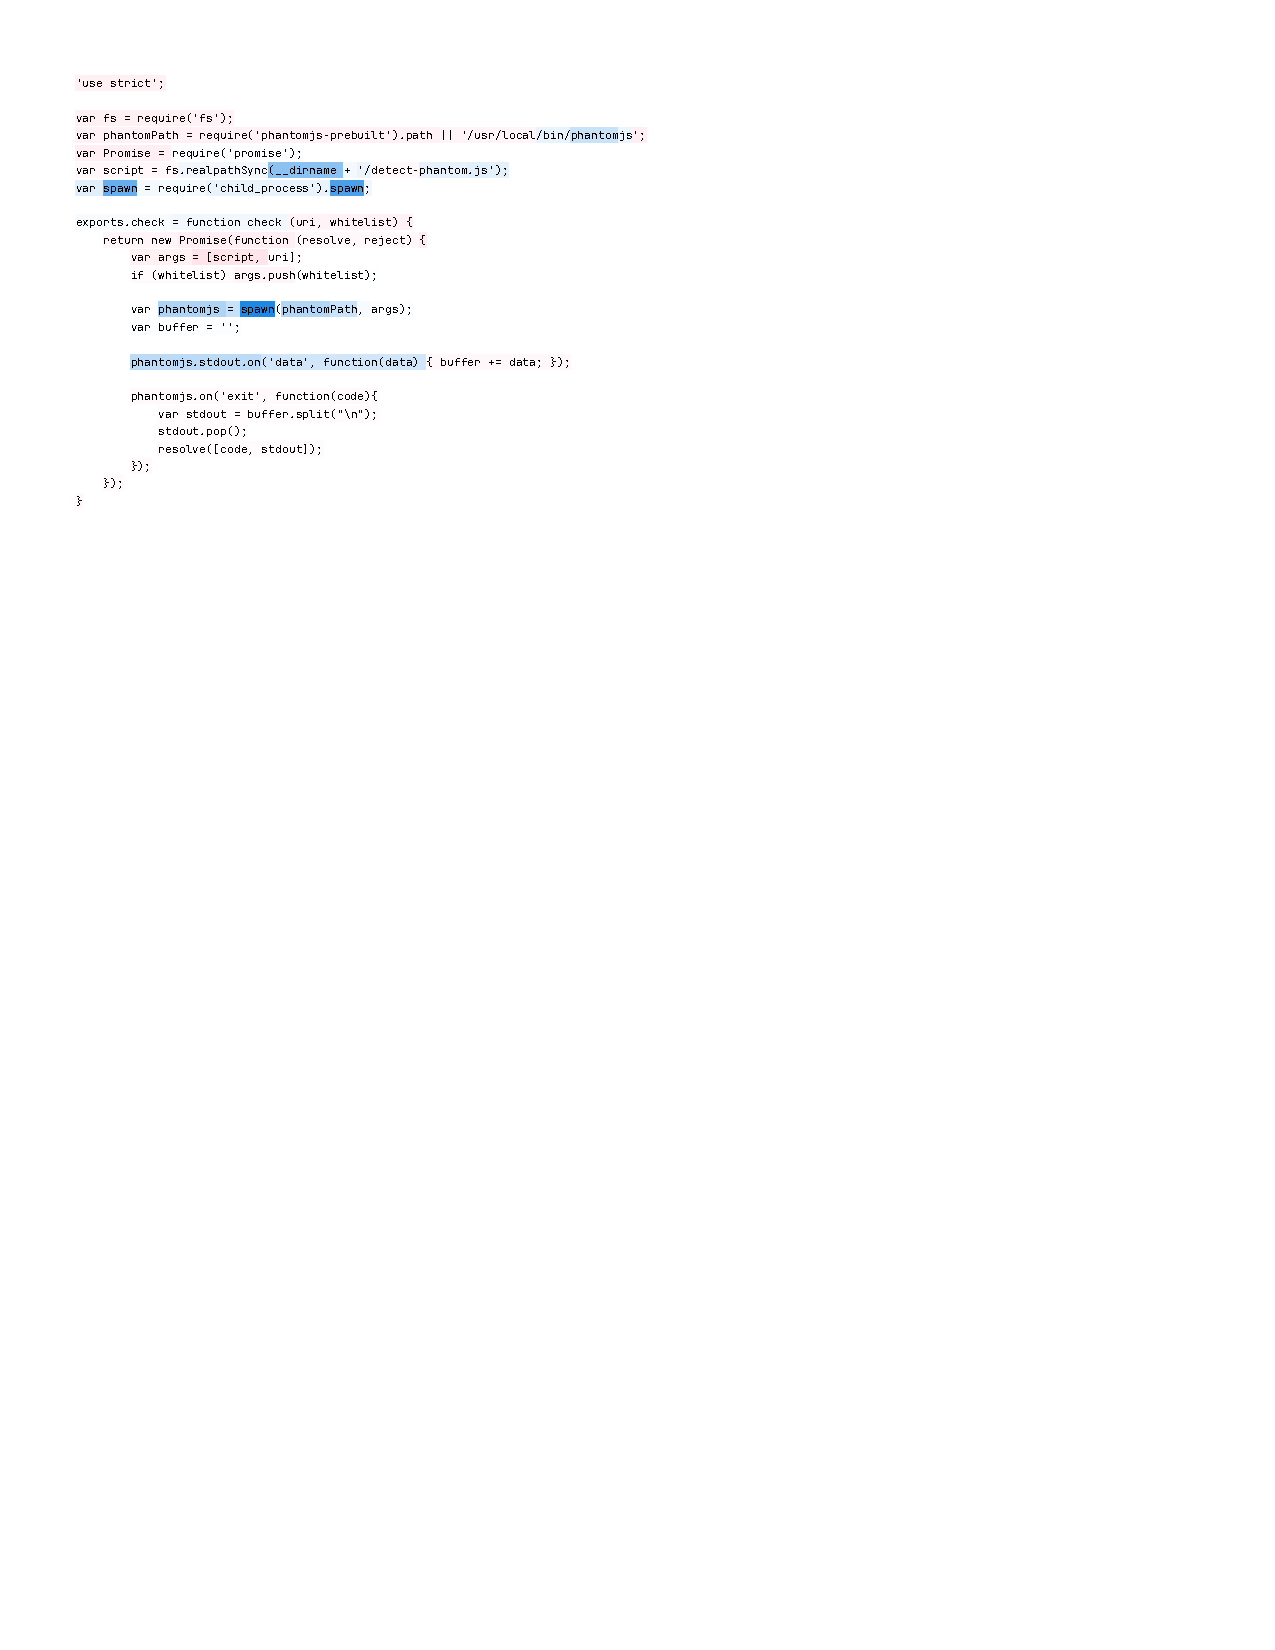
\includegraphics[width=\linewidth]{figures/formatted_code.pdf}
  \vspace{-10pt}
  \caption{Shapley values of the full-fine-tuned DeepSeek-R1-Distill-Qwen-7B on a
  package \textit{third-party-resources-checker}. The correct prediction is: "not vulnerable." Red values indicate a positive contribution to the vulnerable prediction, while blue values indicate a negative contribution. Darker colors represent a higher absolute Shapley value. 
  }
  \label{fig:shapley_spawn}
\end{figure}

Figure \ref{fig:shapley_spawn} is an example of an invulnerable package \textit{third-party-resources-checker}, where the presence of \textit{spawn} is the most significant feature in the prediction after full fine-tuning.
This suggests that the presence of \textit{spawn} is associated with safer execution patterns compared to other process creation functions.

One key reason for this is how \textit{spawn} handles its arguments.
Unlike \textit{exec}, which interprets a string directly as shellcode, 
\textit{spawn} takes a command and its arguments separately as elements of an array,
and takes a second configuration object that only allows for shell meta-character
evaluation if explicitly configured.

This design significantly reduces the risk of command injection attacks because
an attacker must control both the command array and the configuration object
(unless the package itself takes the unsafe action to allow shellcode evaluation).
The need to control multiple arguments was specifically noted by NodeMedic-FINE
as a challenge for confirming/dis-confirming exploitability of \textit{spawn}. 


For other cases, no specific pattern stands out, and most tokens contribute only marginally to the model’s predictions. This suggests that, apart from certain key indicators like \textit{spawn}, the vulnerability classification relies on a distributed set of features rather than any single dominant token. The Shapley values for these other tokens tend to be small and dispersed, indicating that their individual influence on the final prediction is limited.
This behavior supports the idea that security vulnerabilities often result from complex interactions among different parts of the code, rather than being linked to the presence or absence of a single token.

\subsubsection*{Graph-Based Models}
We compared the predictions of \nodemedic{-GNN} with the fully fine-tuned DeepSeek-R1-Distill-Qwen-7B. Among 206 packages in the test split, 178 packages were predicted correctly by the LLM while 189 packages were predicted correct by \nodemedic{-GNN}.
Out of all the predictions on the test split made by LLM and \nodemedic{-GNN}:
171 cases were correctly classified by both classifiers.
10 cases were misclassified by both.

Additionally, we found that \nodemedic{-GNN} and LLMs perform very differently on ACI and ACE vulnerabilities. \nodemedic{-GNN} significantly outperforms LLMs on ACE vulnerabilities, achieving an F1 score of 0.955 compared to 0.889. In contrast, LLMs, along with traditional program analysis methods (i.e., FAST and \nodemedicfine), perform better on ACI than on ACE. This indicates that the \nodemedic{-GNN} and LLMs may concentrate on different aspects of the package when making predictions. However, combining LLMs and GNNs does not always yield better results than using LLMs alone.

\begin{tcolorbox}[colback=white,colframe=black,arc=0pt,boxrule=0.5pt,title=RQ2 Summary,boxsep=2pt,left=1pt,right=1pt,top=1pt,bottom=1pt,fonttitle=\bfseries]
LLMs' identification of non-vulnerable ACI relies on
presence of the \textit{spawn} sink, which is typically safer than \textit{exec}. 
In other cases, no single token determines the prediction.
Graph-based methods exhibit a different prediction distribution to LLMs across the test split, but combining LLMs and GNNs does not always improve performance.
\end{tcolorbox}

\subsection{RQ3: Ablation Study on LLMs}
\label{subsec:rq4}

Our experiments show that the performance of LLMs in the vulnerability detection task is very sensitive to both the base model and the selected usage strategy (e.g., zero-shot, various fine-tuning methods). Table~\ref{tab: main_results} includes key metrics for various LLM-based approaches under different operational configurations, including zero-shot and multiple fine-tuning strategies.

\paragraph{Zero-Shot}
In a zero-shot setting, OpenAI's o3-mini-high model achieves an F1 score of 0.733, which is lower than five out of the seven other models we evaluated for the zero-shot scenario.
However, its metrics—specifically, high precision and moderate recall—are quite similar to those achieved by pure program analysis methods like \nodemedicfine. This suggests that the model tends to be conservative in its predictions.

Among other zero-shot LLMs, all models show fairly similar results, except for DeepSeek-R1-Distill-Qwen-7B and Qwen2.5-Coder-7B-Instruct, which have significantly lower F1 scores. DeepSeek-R1-Distill-Qwen-7B, in particular, sometimes outputs a final answer that contradicts its prior reasoning. The following are two examples where, during the reasoning, the model believes the code is exploitable, but the final answer is "no," and in the other example, it is the opposite.

\begin{tcolorbox}[colback=white, colframe=black]
    \noindent
    \begin{minipage}[t]{0.45\textwidth}
      \small
      \textbf{Output 1:}\\[1ex]
      $<think>$ ... I think \textbf{there are} exploitable ACE vulnerabilities here because the code allows for the execution of arbitrary functions based on the args parameter, which could be controlled by an attacker.
      $</think>$
      \textbf{No}
    \end{minipage}\hfill
    \begin{minipage}[t]{0.45\textwidth}
      \small
      \textbf{Output 2:}\\[1ex]
      $<think>$ ... I think the code \textbf{does not have} any exploitable ACE or ACI vulnerabilities because the unshift method is overridden to do nothing, preventing any code execution.
      $</think>$
      \textbf{Yes}
    \end{minipage}
\end{tcolorbox}

\paragraph{LoRA vs. Full Fine-Tuning}
It is widely believed that a properly hyper-parameter-tuned Low-Rank Adaptation (LoRA) method can achieve performance similar to or even better than full fine-tuning \cite{qlora,lora,mao2025survey}.
We found similar results showing that LoRA fine-tuning performs almost as well as full fine-tuning for most models. For DeepSeek-R1-Distill-Llama-8B and Llama-3.1-8B-Instruct, LoRA fine-tuning even outperforms full fine-tuning. This suggests that LoRA fine-tuning can be a more efficient and effective approach for fine-tuning LLMs, especially when computational resources are limited. Figure \ref{fig:lora_plot} shows the comparison of various LoRA ranks on the models' F1 scores. A sudden increase in the F1 score is observed when the rank is increased, but additional increases in rank do not significantly enhance performance.

\begin{figure}
  \centering
  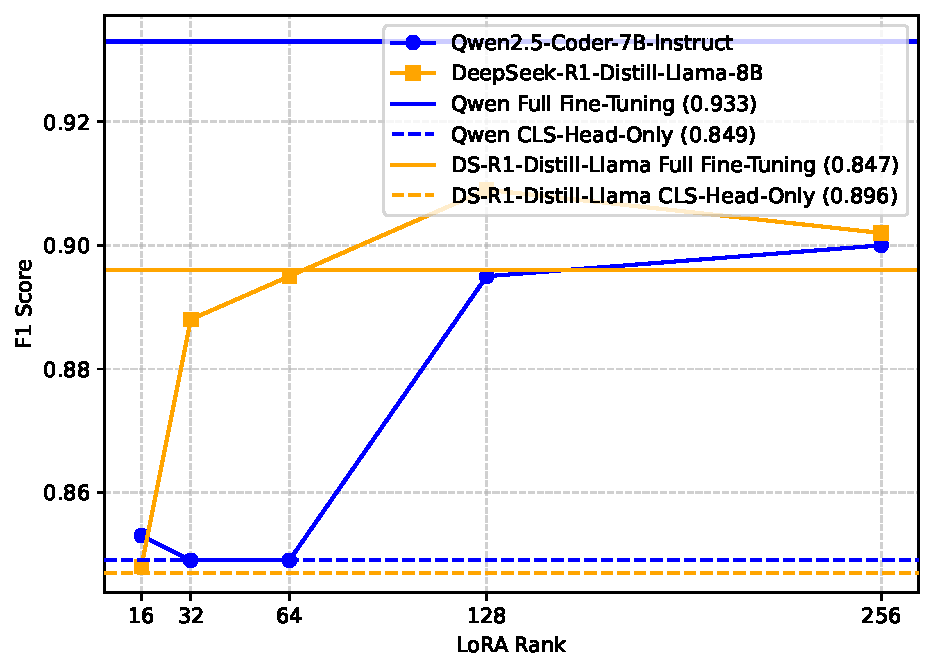
\includegraphics[width=0.6\linewidth]{figures/lora_plot.pdf}
  \caption{Comparison of various LoRA ranks on the F1 score of DeepSeek-R1-Distill-Llama-8B and Qwen2.5-Coder-7B-Instruct. The F1 score is computed based on the test split. Full fine-tuning and classification-head-only fine-tuning are included for comparison.}
  \label{fig:lora_plot}
\end{figure}

\begin{tcolorbox}[colback=white,colframe=black,arc=0pt,boxrule=0.5pt,title=RQ3 Summary,boxsep=2pt,left=1pt,right=1pt,top=1pt,bottom=1pt,fonttitle=\bfseries]
LLM performance in vulnerability detection is highly sensitive to both model choice and usage strategy. In zero-shot settings, most models perform similarly.
LoRA fine-tuning can achieve similar performance to full fine-tuning, and in some cases, it can even outperform full fine-tuning.
\end{tcolorbox}


\subsection{RQ4: Training and Inference Time}


To compare the computational efficiency of LLM-based methods against traditional and ML-enhanced program analysis approaches, we analyze both training time (pre-prediction) and inference time (prediction latency), as presented in Table~\ref{tab: time_overhead}.
All full fine-tuning of the LLMs is performed on four (4) GPUs, unlike other methods for LLMs where experiments are conducted using one (1) GPU. For FAST, the inference time is the median overhead reported in the paper \cite{kang2023scaling} that introduces FAST. The graph generation times of \nodemedicfine represent the average tool runtime reported in the paper \cite{cassel2023nodemedic}, which is 0.79 seconds per output. Some methods of DeepSeek-R1-Distill models are not reported because they share the same model structure as the non-distilled models, and their performance is expected to be similar.

Full fine-tuning or LoRA fine-tuning of LLMs usually takes more training time than ML-enhanced program analysis tools. However, the inference time for fine-tuned LLMs is quicker than that of both program analysis methods and ML-enhanced program analysis methods when processing in batches.
FAST and \nodemedicfine{} provide a PoC exploit, while the other methods cannot.




\begin{tcolorbox}[colback=white,colframe=black,arc=0pt,boxrule=0.5pt,title=RQ4 Summary,boxsep=2pt,left=1pt,right=1pt,top=1pt,bottom=1pt,fonttitle=\bfseries]
LLM-based methods have slightly higher training costs compared to ML-enhanced program analysis methods, but they remain within a reasonable range for practical use. Regarding inference time, fine-tuned LLMs are significantly faster (up to 10 times) than both program analysis methods and ML-enhanced program analysis methods, although the cost of hardware resources should be taken into account.
\end{tcolorbox}




\section{Conclusion}
Our study demonstrates that combining machine learning with program analysis can enhance the results of vulnerability detections in \nodejs packages. 
Our findings show that applying machine learning to outputs from existing program analysis or vulnerability detection tools, or fine-tuning large language models for this task, can significantly improve the performance of vulnerability detection for real world \nodejs packages.
Future work could explore the co-design of program analysis tools and machine learning techniques---particularly advanced deep learning models---as auxiliary components to further enhance their capability to identify vulnerabilities more effectively and accurately.

\chapter{Conclusion}
\label{sec:conclusion}

This dissertation has explored the integration of Large Language Models (LLMs) with traditional program analysis techniques to address critical challenges in software evolution. Through a series of novel approaches and empirical evaluations, I have demonstrated that combining the strengths of LLMs with established software engineering methodologies yields superior results compared to either approach in isolation. My work spans multiple dimensions of software evolution, including fault localization, automated program repair, program transpilation, and security vulnerability detection.

\section{Summary of Contributions}

\subsection{Bidirectional Fine-tuning for Fault Localization}

I developed a bidirectional fine-tuning technique that enables LLMs to perform effective fault localization without relying on pre-written tests (Chapter~\ref{ch:llmao}). By adapting traditionally left-to-right LLMs to understand code in a bidirectional manner, I demonstrated significant improvements in identifying faulty lines of code. This approach not only assists in debugging but also proves effective in detecting runtime security vulnerabilities, addressing a critical gap in existing fault localization techniques.

\subsection{LLM Entropy for Automated Program Repair}

I introduced a novel application of LLM entropy values to enhance automated program repair (Chapter~\ref{ch:entropy}). My research showed that LLM entropy—a measure of model uncertainty—can be leveraged to improve all three critical stages of program repair: fault localization, patch testing efficiency, and plausible patch ranking. The empirical results demonstrated that this hybrid approach outperforms both traditional APR techniques and pure LLM-based methods, achieving an 18\% higher precision in classifying plausible patches while remaining effective for patches produced by modern ML-based tools.

\subsection{Verified Rust Transpilation}

VERT, my verified equivalent Rust transpilation framework, combines LLMs with verification harnesses to ensure functional equivalence between source and target code (Chapter~\ref{ch:vert}). This approach addresses the hallucination problem inherent in LLMs by incorporating formal verification techniques, resulting in transpiled code that is not only functionally correct but also more idiomatic than code produced by traditional transpilers. The evaluation on real-world repositories confirms that this approach strikes an optimal balance between correctness guarantees and code naturalness.

\subsection{Multi-task Security Vulnerability Detection}

Building upon the fault localization work, I extended the approach to security vulnerability detection through multi-task instruction-tuning of LLMs (Chapter~\ref{ch:msivd}). By training models to simultaneously identify vulnerable code and explain exploitation vectors, I created a more comprehensive vulnerability detection system. The experiments demonstrate that this approach effectively detects vulnerabilities spanning multiple files across large repositories, addressing the limitations of line-level fault localization.

\subsection{Hybrid Node.js Vulnerability Detection}

NodeMedic represents a hybrid approach that combines program analysis with LLMs for detecting exploitable vulnerabilities in Node.js packages (Chapter~\ref{ch:nodejs}). By integrating taint provenance tracking with graph neural networks and LLMs, I achieved superior detection performance compared to existing methods. The comprehensive evaluation shows that NodeMedic-GNN achieves an F1 score of 0.943, significantly outperforming traditional program analysis approaches and demonstrating the value of combining multiple techniques for vulnerability detection.

\section{Key Insights and Implications}

Several important insights emerge from this research that have broader implications for the field of software engineering.

While LLMs excel at generating natural, human-like code, they fundamentally operate as black-box models with inherent limitations in understanding program semantics and correctness. My work demonstrates that these limitations can be mitigated by integrating LLMs with traditional program analysis techniques, creating systems that leverage the strengths of both approaches.

The entropy values produced by LLMs during generation provide valuable signals about model uncertainty, which can be harnessed for tasks beyond code generation. This research shows that these entropy values effectively identify potential fault locations and help prioritize candidate patches, offering a novel perspective on how LLM internals can inform software engineering tools.

Verification of LLM outputs is essential for critical software engineering tasks. The transpilation work demonstrates that combining LLM generation capabilities with formal verification techniques produces results that are both correct and natural, addressing a fundamental tension in automated code transformation.

Multi-task learning enables LLMs to develop more nuanced understanding of software vulnerabilities by simultaneously learning to identify vulnerable code and explain exploitation vectors. This approach produces models that can reason about security implications across file boundaries, addressing limitations of traditional vulnerability detection methods.

Most importantly, this research confirms that hybrid approaches combining neural and symbolic methods consistently outperform pure neural or pure symbolic approaches across various software evolution tasks. This finding has significant implications for the design of future software engineering tools, suggesting that the most effective systems will integrate multiple paradigms rather than relying exclusively on either traditional program analysis or deep learning.

\section{Limitations and Future Work}

Despite the advances presented in this dissertation, several limitations remain to be addressed in future work, while recent developments in LLMs present both new opportunities and continued challenges.

The scalability of these approaches to very large codebases remains a challenge, particularly for tasks requiring whole-program analysis. However, recent advances in LLM context windows (with models now supporting millions of tokens) present new opportunities for applying these techniques to larger codebases without the segmentation strategies employed in this work. Future research should explore how these expanded context windows can be leveraged while maintaining the benefits of the hybrid approaches developed here.

While the transpilation work focused on Rust as a target language, extending these techniques to other language pairs would provide valuable insights into the generalizability of the approach. Additionally, exploring bidirectional transpilation (i.e., converting code back to its original language) could serve as an additional verification mechanism. The emergence of agentic LLMs that can autonomously call verification tools presents exciting possibilities for self-checking transpilation systems that could iteratively improve their outputs.

The security vulnerability detection work currently focuses on specific vulnerability types in Node.js applications. Expanding this approach to cover a broader range of vulnerability classes and programming languages would increase its practical utility. Modern LLMs demonstrate improved zero-shot performance on fault localization tasks, potentially reducing the need for extensive fine-tuning. However, the specialized knowledge captured through the fine-tuning approaches in this dissertation (particularly the multi-task learning for vulnerability explanation) remains valuable for achieving high precision in security-critical applications.

The interpretability of hybrid neural-symbolic systems remains limited, making it difficult for developers to understand why certain code is flagged as vulnerable or why specific repairs are suggested. Future work should explore techniques for making these systems more transparent and explainable, potentially leveraging the improved reasoning capabilities of newer LLMs to provide better explanations of their decisions.

Despite rapid advances in LLM capabilities, there remains significant value in the program analysis integration and fine-tuning optimization techniques presented in this work. Models continue to be expensive to pre-train, and the techniques developed in this thesis can be valuable for generating higher quality training data without dependency on human labelers. The entropy-based approaches for patch ranking and the multi-task learning frameworks can serve as automated data curation mechanisms, identifying high-quality code examples and vulnerability patterns for training future models.

Reinforcement learning presents an underexplored opportunity, particularly for security-related data flows. The provenance graphs and taint analysis techniques developed in this work could serve as reward signals for reinforcement learning systems, enabling models to learn optimal security practices through interaction with program analysis tools. This could lead to LLMs that not only detect vulnerabilities but also learn to write more secure code through reinforcement.

The parameter-efficient fine-tuning techniques (e.g., LoRA) demonstrated in this work remain relevant even as base models grow larger. These approaches enable rapid adaptation of large models to specific domains and tasks without the computational overhead of full fine-tuning, making specialized software engineering applications more accessible to researchers and practitioners with limited computational resources.

Future work should also investigate how the hybrid approaches developed here can be adapted to leverage emerging LLM capabilities while maintaining their core advantages. For instance, combining the bidirectional fine-tuning techniques with modern instruction-following models could yield even more effective fault localization systems, while the verification frameworks developed for transpilation could be extended to work with agentic systems that can autonomously invoke multiple verification tools.

\section{Concluding Remarks}

This dissertation has demonstrated that software engineering is indeed an evolving process that benefits from a holistic understanding of software properties. By addressing the limitations of LLMs through integration with program analysis techniques, I have created effective tools for fault localization, automated program repair, program transpilation, and security vulnerability detection.

The work contributes to a growing body of evidence suggesting that the future of software engineering tools lies not in replacing traditional techniques with deep learning, but in thoughtfully combining them to create systems that leverage the strengths of both approaches. As software systems continue to grow in complexity and importance, such hybrid approaches will be essential for maintaining software quality, security, and evolvability.

The tools and techniques presented in this dissertation are open-source and available to the research community, providing a foundation for future work in this rapidly evolving field. I hope that these contributions will inspire further research into the integration of LLMs with traditional software engineering methodologies, ultimately leading to more powerful and practical tools for software evolution.



\backmatter
\renewcommand{\bibsection}{\chapter{\bibname}}
\bibliographystyle{plainnat}
\bibliography{dissertation} 
\end{document}
